\documentclass[12pt,MSc]{muthesis_2023}
%This is not a thesis. Do not call it a paper either.
%Single-sided printing for producing pdf to be read on screen.
%No need for wordcount.

% add a few important packages 
\usepackage{amsmath}
\usepackage{amsfonts}
\usepackage{amssymb}
\usepackage{lipsum}
\usepackage[utf8]{inputenc}
\usepackage{graphicx}
\usepackage{stmaryrd} % Required for inserting images
\usepackage{tikz}
\usepackage{dsfont}
\usepackage{hyperref}

\bibliography{refs}

% Listing package to control how code appears in your document
\usepackage{listings}
\lstset{language=c++,frame=single,showstringspaces=false,basicstyle=\footnotesize,breaklines=true,keywordstyle=\color{blue},commentstyle=\color{grey},stringstyle=\color{red},identifierstyle=\color{green}}

\usepackage{hyperref}

\usepackage{float}


\usepackage{chngcntr}
\counterwithout{equation}{section} % Stop equation counter from resetting with section
\renewcommand{\theequation}{E.\arabic{equation}} % Change display to E.number


\let\oldemph\emph
\renewcommand{\emph}[1]{\textbf{\textit{#1}}}
\usepackage{amsthm} % Theorem environments
\usepackage{amsmath}
\usepackage{enumitem}
\usepackage{amsfonts}
\usepackage{listings}
\usepackage{tcolorbox}
\usepackage{amssymb}
\usepackage{mathtools}

\newcounter{resCounter}[section]

% -- How each result is labeled: "section.counter"
\renewcommand{\theresCounter}{\thesection.\arabic{resCounter}}

% -- Define a custom theorem style without newline for Remarks & Observations
\newtheoremstyle{nonbreakthm}%
{10pt}    % Space above
{10pt}    % Space below
{\normalfont} % Body font
{}        % Indent amount
{}  % Theorem head font (bold)
{:}        % Punctuation after theorem head
{ }        % Space after theorem head (no newline, just a space)
{\textbf{\thmname{#1} \thmnumber{#2}}\thmnote{ (#3)}} % Heading spec

% -- Define a custom theorem style for theorems, lemmas, propositions (with newline)
\newtheoremstyle{mythmstyle}%
{10pt}    % Space above
{10pt}    % Space below
{\normalfont} % Body font (upright, not italic)
{}        % Indent amount
{}  % Theorem head font (bold)
{:}        % Punctuation after theorem head
{\newline} % Space after theorem head (forces the body onto a new line)
{\textbf{\thmname{#1} \thmnumber{#2}}\thmnote{ (#3)}} % Heading spec

% -- Activate styles accordingly
\theoremstyle{mythmstyle}
\newtheorem{definition}[resCounter]{Definition}
\newtheorem{lemma}[resCounter]{Lemma}
\newtheorem{proposition}[resCounter]{Proposition}
\newtheorem{theorem}[resCounter]{Theorem}
\newtheorem{corollary}[resCounter]{Corollary}
\newtheorem{notenl}[resCounter]{Note}
\newtheorem{remarknl}[resCounter]{Remark}
\newtheorem{exercise}[resCounter]{Exercise}

\theoremstyle{nonbreakthm}
\newtheorem{note}[resCounter]{Note}
\newtheorem{observation}[resCounter]{Observation}
\newtheorem{example}[resCounter]{Example}
\newtheorem{question}[resCounter]{Question}
\newtheorem{remark}[resCounter]{Remark}
% This command repeats \blacksquare n times (no numbers printed).
\NewDocumentCommand{\RepeatBlackSquares}{m}
 { \blacksquare\kern0.2em }

\ExplSyntaxOff

% Our custom subproof environment:
%   1st optional arg = proof title   (default \proofname)
%   2nd optional arg = number of squares (default 1)
\NewDocumentEnvironment{subproof}{O{\proofname} O{1}}
{
    \renewcommand{\qedsymbol}{\RepeatBlackSquares{#2}}
    \begin{proof}[#1]
    }
    {
    \end{proof}
}


\makeatletter
\renewenvironment{proof}[1][\proofname]{\par
\pushQED{\qed}%
\normalfont \topsep6\p@\@plus6\p@\relax
\trivlist
\item[\hskip\labelsep
\itshape
#1\@addpunct{:}]\leavevmode\\[-3ex]  % smaller vertical space than \mbox{}\\*
}{%
\popQED\endtrivlist\@endpefalse
}
\makeatother
%#######

\begin{document}
    %This should be the original project title. Any changes should be agreed with your supervisor.
\title{TODO}

%Put your name here
\author{Vorashil Farzaliyev}

%It will say Department of Mathematics
\school{Mathematics}
\faculty{Science and Engineering}

\beforeabstract

Write your abstract here: Remember, it must fit on this A4 page and should
describe contents of the dissertation. Here might also be a good place
to indicate what you have achieved in the dissertation. Do not call your dissertation a thesis or a paper.


\afterabstract

% The next part is optional; however it is a good place to thank your
% supervisor and the people responsible for providing computer support ;-)
\prefacesection{Acknowledgements}
I would like to thank...

% The next line is NOT optional and MUST appear
\afterpreface


% Finally, you can start writing your dissertation


    \chapter{Motivation and Preliminaries}\label{ch:preliminaries}


\section{Motivation}

\subsection{Notations}\label{subsec:notations}

We denote the set of positive natural numbers by $\mathbb{N}$ and use $\mathbb{N}_0 =\mathbb{N} \cup \{0\}$. Given $m \in \mathbb{N}$, we use
\[
    [m] = \{1, 2, \ldots, m\} \textrm{ and }  [m]_0 = \{0, 1, 2, \ldots, m\}.
\]

\noindent
We denote the tuples by using underlying letters such as $\underline{z} = (z_1, \dots, z_n)$ for some $n \in \mathbb{N}$. Write $A \subseteq X$ for a subset of arbitrary set $X$. Then the powerset of  $A$ is denoted as $\mathcal{P}(A)$, which is the collection of all subsets of $A$. If $f : X \to \mathbb{R}$ is real valued functions, the restriction of $f$ to a subset $A \subseteq X$ is denoted by $f|_A$.

\subsection{Pre-requisites to read this dissertation}

In the next sections, we include some preliminary concepts that can be found in more generality in other literature as a standard graduate mathematics course. However, to aim this dissertation for the someone with background in model theory only, we have added a section of required concepts from probability theory and introduce notations that will be useful for the later discussions of learning theory. In general, the definition of learning is formally described using the language of probability theory \cite[Chap 2]{MartinAnthony}. Moreover, the probability theory itself is formalised using the language of measure theory, so it's crucial to understand the concepts of measure theory and model theory. The topics on Measure theory closely follows the presentation of \cite{MeasureTheoryLeGall}.



\begin{table}[H]
    \centering
    \renewcommand{\arraystretch}{1.3}
    \begin{tabular}{|p{3cm}|p{3cm}|p{3cm}|p{3cm}|}
        \hline
        &
        \textbf{Probability Theory}
        &
        \textbf{Model Theory}
        &
        \textbf{Measure Theory} \\
        \hline
        Structure
        &
        $(\Omega,\mathcal{F},P)$
        &
        Structure $\mathcal{M}$, formulas $\varphi$, $\psi$
        &
        $(X,\Sigma,\mu)$ \\
        \hline
        $A,B$ &
        Events $A,B\in\mathcal{F}$
        &
        Definable sets \newline
        $\varphi(\mathcal{M}), \psi(\mathcal{M}) \subseteq M^n$
        &
        Measurable sets $A,B\in\Sigma$ \\
        \hline
        $A \lor B$
        &
        $A\cup B \in \mathcal{F}$
        &
        $(\varphi \lor \psi)(\mathcal{M}) \subseteq M^n$ is definable.
        &
        $A\cup B \in \Sigma$ \\
        \hline
        $A \land B$
        &
        $A\cap B \in \mathcal{F}$
        &
        $(\varphi \land \psi)(\mathcal{M}) \subseteq M^n$ is definable.
        &
        $A\cap B \in \Sigma$ \\
        \hline
        $\lnot A$
        &
        $A^c \in \mathcal{F}$
        &
        $\lnot\varphi(\mathcal{M})  \subseteq M^n$ is definable.
        &
        $X\setminus A \in \Sigma$ \\
        \hline
    \end{tabular}
    \caption{Logical operations in three frameworks.}\label{tab:table-comparison}
\end{table}

\section{Measure Theory}\label{sec:measure-theory}

Measure theory provides a rigorous framework for extending the notions of length, area, and volume to more abstract sets. Its central object is a \emph{measure}: a function that assigns a numerical value to subsets, interpreted as their ``size.'' In standard measure theory, a measure must be \textit{non-negative} and satisfy \textit{countable additivity}, meaning that the measure of a countable union of pairwise disjoint sets equals the sum of the measures of the individual sets. However, it is impossible to define a measure with these properties on all subsets of a given space~\cite[Sec.~1.1]{MeasureTheoryTao}. The usual resolution is to restrict attention to a distinguished collection of subsets, called \emph{measurable sets}, which form a \emph{$\sigma$-algebra}. This structure is crucial because it is closed under countable set operations, ensuring that measurable sets remain measurable under unions, intersections, and complements, and that the principle of countable additivity is well defined.

This section introduces the foundational concepts from measure theory required to formalize the notion of a probability space. This formalism is essential for the rigorous treatment of learning theory in Chapter~\ref{ch:pac-learning}. Our presentation closely follows~\cite{MeasureTheoryCohn} and~\cite{MeasureTheoryLeGall}. Throughout this section, we let $X$ be an arbitrary set and its power set, the collection of all its subsets, is denoted by $\mathcal{P}(X)$.

\subsection{$\sigma$-algebras}

We begin by defining the structure that characterizes the collection of measurable sets.

\begin{definition}[$\sigma$-algebra \textnormal{\cite[Def.~1.1]{MeasureTheoryCohn}}]
    \label{def:sigma-algebra}
    A \emph{$\sigma$-algebra} on a set $X$ is a collection $\mathcal{A} \subseteq \mathcal{P}(X)$ such that:
    \begin{enumerate}[label=(\roman*)]
        \item $X \in \mathcal{A}$,
        \item if $E \in \mathcal{A}$, then $X \setminus E \in \mathcal{A}$,
        \item if $E_i \in \mathcal{A}$ for $i \in \mathbb{N}$, then
        \[
            \bigcup_{i=1}^\infty E_i \in \mathcal{A} \quad \text{and} \quad \bigcap_{i=1}^\infty E_i \in \mathcal{A}.
        \]
    \end{enumerate}
\end{definition}

\medskip

From Definition~\ref{def:sigma-algebra} several basic consequences follow. First, $\emptyset \in \mathcal{A}$ since $\emptyset = X \setminus X$. Second, $\sigma$-algebras are closed under finite unions and finite intersections: for the union, note that if $E_1, \dots, E_k \in \mathcal{A}$, then
\[
    \bigcup_{i=1}^k E_i = \bigcup_{i=1}^\infty F_i \quad \text{where }
    F_i =
    \begin{cases}
        E_i & 1 \leq i \leq k,\\
        \emptyset & i > k,
    \end{cases}
\]
and similarly finite intersections follow from De Morgan’s law and closure under complements.

\medskip
An important observation is that the intersection of an arbitrary family of $\sigma$-algebras on a set $X$ is itself a $\sigma$-algebra~\cite[Prop.~1.1.2]{MeasureTheoryCohn}. This fact makes it possible to define the \emph{smallest} $\sigma$-algebra containing a given collection of subsets. Indeed, given $\mathcal{C} \subseteq \mathcal{P}(X)$, one may consider the intersection of all $\sigma$-algebras on $X$ that contain $\mathcal{C}$. By~\cite[Cor.~1.1.3]{MeasureTheoryCohn}, this intersection is guaranteed to exist and yields the minimal $\sigma$-algebra containing $\mathcal{C}$. We record this construction in the following definition.

\begin{definition}[$\sigma$-algebra generated by a collection \textnormal{\cite[Def.~1.2]{MeasureTheoryLeGall}}]
    \label{def:sigma-generated}
    Let $\mathcal{C} \subseteq \mathcal{P}(X)$. The \emph{$\sigma$-algebra generated by $\mathcal{C}$}, denoted $\sigma(\mathcal{C})$, is the intersection of all $\sigma$-algebras on $X$ that contain $\mathcal{C}$. Equivalently, $\sigma(\mathcal{C})$ is the smallest $\sigma$-algebra on $X$ such that $\mathcal{C} \subseteq \sigma(\mathcal{C})$.
\end{definition}

This notion of generation also provides a natural way to define the \emph{product $\sigma$-algebra}. Given $\sigma$-algebras $\mathcal{A}_1$ on $X_1$ and $\mathcal{A}_2$ on $X_2$, we first consider the collection of measurable rectangles $\{A_1 \times A_2 \mid A_1 \in \mathcal{A}_1, A_2 \in \mathcal{A}_2\}$. These rectangles alone do not form a $\sigma$-algebra, but we can generate one by closing under the operations of complements and countable unions. This leads to the following definition.

\begin{definition}[Product $\sigma$-algebra \textnormal{\cite[Def.~1.4]{MeasureTheoryCohn}}]
    \label{def:product-sigma-algebra}
    Let $X_1, X_2$ be sets and $\mathcal{A}_1, \mathcal{A}_2$ $\sigma$-algebras on them, respectively. The \emph{product $\sigma$-algebra} $\mathcal{A}_1 \otimes \mathcal{A}_2$ is the smallest $\sigma$-algebra containing all measurable rectangles:
    \[
        \mathcal{A}_1 \otimes \mathcal{A}_2 \coloneq \sigma\bigl(\{A_1 \times A_2 \mid A_1 \in \mathcal{A}_1, \, A_2 \in \mathcal{A}_2\}\bigr).
    \]
\end{definition}

\subsection{Measure space}

Let $X$ be a set and $A \subseteq X$ be a subset. It's natural to ask "what would be the \texit{size} or \textit{measure} of the subset $A$ relative to $X$". However, it's also natural to follow up and ask "what would be the size of $X$". In essence, this relativity part of this question distinguish probability theory from more generic measure theory. It's because, in probabily theory we set the size of $X$ as $1$, in which case, we can compare the size of \textit{measurable} subset $A$ to the size of $X$. However, in general, measure theory we don't have any such assumption on $X$ other than the assumption that $X$ is itself measurable. Note that, in our original question we also make an assumption about \textit{measurability} of $A$, which will be formalised using $\sigma$-algebras.

\begin{definition}[Measurable space]
    A measurable space is a pair $(X, \mathcal{A})$, where $X$ is a set and $\mathcal{A}$ is a $\sigma$-algebra on $X$. The elements of $\mathcal{A}$ are called \emph{measurable sets}.
\end{definition}

If we have a measurable space $(X, \mathcal{A})$, the logical step is to define a measure for all $A \in \mathcal{A}$. In this dissertation we will assume that measure is always non-negative real function $\mathcal{A} \to [0, \infty)$. We will call the measurable space $(X,\mathcal{A})$ with associated measure function $\mu$ as \emph{measure space} and denote it by the triple $(X, \mathcal{A}, \mu)$. The definition of such measure functions is as follows:

\begin{definition}[Measure]
    A measure $\mu$ on a measurable space $(X, \mathcal{A})$ is a function $\mu: \mathcal{A} \to [0, +\infty]$ satisfying:
    \begin{enumerate}[label=(\roman*)]
        \item $\mu(\emptyset) = 0$,
        \item $\mu(E) < +\infty$ for all $E \in \mathcal{A}$,
        \item if $E_i \in \mathcal{A}$ for $i \in \mathbb{N}$ are pairwise disjoint sets, then
        \[
            \mu\left(\bigcup_{i=1}^\infty E_i\right) = \sum_{i=1}^\infty \mu(E_i).
        \]
    \end{enumerate}
\end{definition}

\begin{notenl}
    Some important special cases and notions related to measures:
    \begin{itemize}
        \item A measure $\mu$ is called \emph{finite} if $\mu(X) < \infty$.
        \item A measure $\mu$ is a \emph{probability measure} if $\mu(X) = 1$. In this case, the triple $(X, \mathcal{A}, \mu)$ is called a \emph{probability space}.
        \item A point $x \in X$ is said to be an \emph{atom} of the measure $\mu$ if $\mu(\{x\}) > 0$.
    \end{itemize}
\end{notenl}

One of the important special cases of a measure will be Dirac measure that's based on \emph{indicator functions} (also known as a characteristic function) $\mathds{1}_A: X \to \{0, 1\}$ for a set $A \subseteq X$ and is defined as
\begin{equation}
    \label{eq:indicator-function-def}
    \mathds{1}_A: X \to \{0, 1\}, \quad \mathds{1}_A(x) =
    \begin{cases}
        1 & \text{if } x \in A, \\
        0 & \text{if } x \notin A.
    \end{cases}
\end{equation}
These functions provide a convenient way to express membership in a set and are fundamental to the construction of measures and integration theory.


\begin{definition}[Dirac Measure]
%    taken from the paper
    Given a measurable space $(\Omega, \Sigma)$, where $\Sigma \subseteq \mathcal{P}(\Omega)$ and an element $\omega \in \Omega$, we denote the \emph{Dirac measure} $\delta_{\omega}: \Sigma \to \{0, 1\}$ as
    \[
        \begin{aligned}
            \delta_{\omega}: \Sigma &\to \{0, 1\} \\
            A &\mapsto \delta_{\omega}(A) = \mathds{1}_A(\omega)
        \end{aligned}
    \]
\end{definition}

\subsection{Borel $\sigma$-algebra}

Throughout this dissertation, we will focus on a particular class of $\sigma$-algebras that naturally arise in the context of topological spaces. Let $(X, \tau)$ be a topological space, where $\tau \subseteq \mathcal{P}(X)$ denotes the collection of open sets in $X$. The $\sigma$-algebra generated by $\tau$, denoted by $\sigma(\tau)$ (see~\ref{eq:generated-sigma-algebra-def}), is called the \emph{Borel $\sigma$-algebra} on $X$ and is written as
\[
    \mathcal{B}(X) \coloneq \sigma(\tau).
\]

\begin{example}[Borel $\sigma$-algebra on $\mathbb{R}$]
    Consider the metric space $(\mathbb{R}, d)$, where $d$ is the Euclidean metric. The open sets in $\mathbb{R}$ are generated by the open intervals $(a, b)$ with $a, b \in \mathbb{R}$ and $a < b$. Therefore, the Borel $\sigma$-algebra $\mathcal{B}(\mathbb{R})$ is the smallest $\sigma$-algebra containing all open intervals. Equivalently, $\mathcal{B}(\mathbb{R})$ can also be generated by half-open rays of the form $(-\infty, a)$ for $a \in \mathbb{R}$. This flexibility in generators will be useful later when we discuss measurability of functions.
\end{example}

\begin{lemma}[Product of Borel $\sigma$-algebras \textnormal{\cite[Lemma 1.5]{MeasureTheoryLeGall}}]
    \label{lem:product-borel-sigma}
    Suppose that $E$ and $F$ are separable metric spaces, and equip the product $E \times F$ with the product topology. Then
    \[
        \mathcal{B}(E \times F) = \mathcal{B}(E) \otimes \mathcal{B}(F).
    \]
\end{lemma}

\begin{remarknl}
    An important application of~\ref{lem:product-borel-sigma} is the case $E = F = \mathbb{R}$. In this setting, we obtain
    \[
        \mathcal{B}(\mathbb{R}^2) = \mathcal{B}(\mathbb{R}) \otimes \mathcal{B}(\mathbb{R}).
    \]
    This identification is fundamental: it guarantees that the Borel structure on the Euclidean plane $\mathbb{R}^2$ coincides with the product $\sigma$-algebra generated by intervals of the form $(a, b) \times (c, d)$. In particular, this fact underpins the rigorous construction of multivariate random variables and joint distributions. Without this identification, extending probability theory from one-dimensional random variables to higher-dimensional vectors would not be straightforward.
\end{remarknl}

\subsection{Measurable functions}\label{subsec:measurable-functions}

So far, we have introduced measurable spaces and measures. The next step is to formalize the notion of functions that are compatible with these structures. Such functions are called \emph{measurable functions}. This concept will allow us to define random variables in the next section~\ref{def:random-variable-prob}.

\begin{definition}[Measurable function \textnormal{\cite[Def.~1.8]{MeasureTheoryCohn}}]
    \label{def:measurable-function}
    Let $(X, \mathcal{A})$ and $(Y, \mathcal{B})$ be measurable spaces. A function $f : X \to Y$ is said to be \emph{measurable} if
    \[
        \forall B \in \mathcal{B}, \quad f^{-1}(B) \in \mathcal{A}.
    \]
    When $X$ and $Y$ are topological spaces equipped with their respective Borel $\sigma$-algebras, we also say that $f$ is \emph{Borel measurable}.
\end{definition}


\begin{example}
    We have come across some measurable functions already and it's useful to recall them.
    \label{ex:measurable-functions}

    \begin{enumerate}
        \item Let $(X, \mathcal{A})$ be a measurable space. For any $A \in \mathcal{A}$, the indicator function~\ref{eq:indicator-function-def} $\mathds{1}_A: X \to \{0, 1\}$ is measurable.
        \item Let $(X_1, \mathcal{A}_1), \dots, (X_n, \mathcal{A}_n)$ be measurable spaces. Consider the product measurable space $(\Pi_{i=1}^n X_i, \otimes_{i=1}^n \mathcal{A}_i)$, where $\Pi_{i=1}^n X_i$ is cartesian product of $X_i$s and $\otimes_{i=1}^n \mathcal{A}_i$ is product $\sigma$-algebra defined in~\ref{def:product-sigma-algebra}. Then the canonical projection $\pi_i: \Pi_{i=1}^n X_i \to X_i$, for $1 \leq i \leq n$ is measurable, since for any $A \in \mathcal{A}_i$,
        \[
            \pi^{-1}(A) = X_1 \times \dots \times A_i \times \dots \times X_n \in \bigotimes_{i=1}^n \mathcal{A}_i.
        \]
        It's important to note here that the product $\sigma$-algebra $\otimes_{i=1}^n \mathcal{A}_i$ is the smallest such algebra on $\Pi_{i=1}^n X_i$ that makes the canonical projection map $\pi_i$ measurable~\cite[\S 8.1, p.243]{MeasureTheoryCohn}.
    \end{enumerate}

\end{example}

There is a direct analogy between the definition of a continuous function in topology and that of a measurable function in measure theory~\cite[Cor.~2.2]{FollandRealAnalysis}. In topology, a function is continuous if the preimage of every open set is open. Similarly, a function is measurable if the preimage of every measurable set belongs to a given $\sigma$-algebra. To emphasize the role of the $\sigma$-algebra $\mathcal{A}$—just as continuity is relative to the topology on the domain—we often say that a function $f$, as in~\ref{def:measurable-function}, is \emph{$\mathcal{A}$-measurable}. In probability theory, $\mathcal{A}$ typically denotes the $\sigma$-algebra of events, in which case measurable functions correspond precisely to random variables.

\begin{remarknl}
    \label{rem:measurable-functions}
    Measurable functions satisfy the following useful properties:
    \begin{enumerate}
        \item The composition of two measurable functions is measurable~\cite[Prop.~1.9]{MeasureTheoryCohn}.
        \item Let $(X, \mathcal{B}(X))$ be a measurable space where $\mathcal{B}(X)$ denotes the Borel $\sigma$-algebra. If $f, g : X \to \mathbb{R}$ are measurable, then so are $f+g$ and $fg$. A stronger version holds for $f, g : X \to \mathbb{C}$~\cite[Prop.~2.6]{FollandRealAnalysis}. Moreover, a function $f : X \to \mathbb{C}$ is measurable if and only if its real and imaginary parts $\Re(f), \Im(f) : X \to \mathbb{R}$ are measurable~\cite[Cor.~2.5]{FollandRealAnalysis}. Hence, the measurability results for real-valued functions extend directly to the complex-valued case.
    \end{enumerate}
\end{remarknl}

As an application of the second property, we obtain the following result.

\begin{corollary}
    Let $(X, \mathcal{B}(X))$ be a measurable space and let $f, g : X \to \mathbb{R}$. Suppose $f$ is measurable and $g$ is non-measurable. Then $g-f$ is not measurable.
\end{corollary}

\begin{proof}

    Assume, for the sake of contradiction, that $h \coloneq g - f$ is measurable. Then, by the second property in~\ref{rem:measurable-functions}, the function $h+f$ is measurable. But $h+f = g$, which contradicts the assumption that $g$ is non-measurable. Hence $h$ is not measurable.
\end{proof}

A useful sufficient condition for measurability is the following (see~\cite[Prop.~1.9]{MeasureTheoryLeGall}):

\begin{proposition}
    \label{prop:measurability-sufficient-cond}
    Let $(X, \mathcal{A})$ and $(Y, \mathcal{B})$ be measurable spaces, and let $f : X \to Y$. In order for $f$ to be measurable, it suffices that there exists a subclass $\mathcal{C} \subseteq \mathcal{B}$ such that $\sigma(\mathcal{C}) = \mathcal{B}$ and
    \[
        f^{-1}(C) \in \mathcal{A}, \quad \forall C \in \mathcal{C}.
    \]
\end{proposition}

\begin{example}
    Suppose $(Y, \mathcal{B}) = (\mathbb{R}, \mathcal{B}(\mathbb{R}))$. To verify that $f$ is measurable, it suffices to check that for every $a < b$, the preimages $f^{-1}((a,b))$ are measurable. In fact, it is already enough to check measurability for sets of the form $f^{-1}((-\infty,a))$, with $a \in \mathbb{R}$.
\end{example}


%
%\subsection{Rigorous definition of Random variable}
%
%Recall that, a probability space is a triple $(\Omega, \mathcal{F}, P)$, where $\Omega$ is a sample space, $\mathcal{F}$ is a $\sigma$-algebra on $\Omega$, called events, and $P$ is a probability measure on $(\Omega, \mathcal{F})$. The measure $P$ assigns probabilities to events in $\mathcal{F}$.
%
%
%\begin{definition}[Random variable]
%    Let $(\Omega, \mathcal{F}, P)$ be a probability space where
%    \begin{itemize}
%        \item $\Omega$ is a sample space
%        \item $\mathcal{F}$ is a $\sigma$-algebra on $\Omega$
%        \item and $P: \mathcal{F} \to [0, 1]$ is a probability measure on $(\Omega, \mathcal{F})$.
%    \end{itemize}
%    Write $\mathcal{B}(\mathbb{R})$ be the Borel $\sigma$-algebra on $\mathbb{R}$. A function $X : \Omega \to \mathbb{R}$ such that
%    for all $B \in \mathcal{B}(\mathbb{R})$
%    \[
%        X^{-1}(B) = \{w \in \Omega: X(w) \in B\} \in \mathcal{F}
%    \]
%    is said to be a \emph{random variable} on $\Omega$.
%\end{definition}



\section{Probability Theory}\label{sec:probability-theory}


\indent
The central aim of modern probability theory is to provide a rigorous mathematical framework for modeling and analyzing phenomena involving uncertainty or randomness. This is achieved by building upon the foundations of measure theory, where probabilistic concepts are given precise measure-theoretic interpretations. The axiomatic framework, established by Andrey Kolmogorov, recasts probability in the language of measure spaces, where the "size" of a set of outcomes corresponds to its likelihood ~\cite[Chap 8]{MeasureTheoryLeGall}.

Just as measure theory confronts the impossibility of assigning a measure to all subsets of a general set (e.g., Vitali sets), probability theory restricts its focus to a collection of "events" that form a $\sigma$-algebra. An event is simply a set of possible outcomes to which a probability can be assigned. This structure ensures that logical combinations of events (e.g., "A or B", "A and B", "not A") are also events with well-defined probabilities.

\subsection{Probability Spaces}


\begin{definition}[Probability Space \textnormal{\cite{DurrettProbability}}]
    \label{def:probability-space}
    A \emph{probability space} is a measure space $(\Omega, \mathcal{F}, \mathbb{P})$ where:
    \begin{enumerate}[label=(\roman*)]
        \item $\Omega$ is a non-empty set, called the \emph{sample space}.
        \item $\mathcal{F}$ is a $\sigma$-algebra on $\Omega$. Its elements are called \emph{events}.
        \item $\mathbb{P}:\mathcal{F} \to [0, 1]$ is a \emph{probability measure} on $(\Omega, \mathcal{F})$, which is a measure satisfying the additional property that $\mathbb{P}(\Omega) = 1$.
    \end{enumerate}
\end{definition}

We will make a notational distinction between the general measure-theoretic framework and its probabilistic counterpart. In the former, we deal with a measure space $(X, \mathcal{A}, \mu)$, while in the latter, we work with a probability space $(\Omega, \mathcal{F}, \mathbb{P})$. The transition from measure theory to probability theory is straightforward: we simply impose the additional constraint that the total measure of the sample space $\Omega$ is $1$, thereby transforming our general measure into a probability measure. However, in probability theory, we are interested in mathematical model of random phenomena, where the sample space $\Omega$ represents all possible outcomes, and the $\sigma$-algebra $\mathcal{F}$ contains events of interest.


\begin{example}{\label{ex:probability-space}}
    It's worth noting some simple examples of probability spaces:
    \begin{itemize}
        \item \textbf{Rolling a die twice:} The sample space is $\Omega = \{1, 2, 3, 4, 5, 6\}^2$. Again, we take $\mathcal{F} = \mathcal{P}(\Omega)$. Then for any event $A \subseteq \Omega$, we define the probability measure $\mathbb{P}$ by
        \[
            \mathbb{P}(A) = \frac{|A|}{36},
        \]
        \item \textbf{Rolling a die until we get 6:} Here the sample space is not finite. It's possible that we roll the die 1000 times and not get a 6, even though the probability of this happening is very small. In this case, the sample space is
        \[
            \Omega = \{1, 2, 3, \dots, 6\}^{\mathbb{N}},
        \]
        while $\mathcal{F}$ is the smallest $\sigma$-algebra containing all sets of the form
        \[
            \{\omega \in \Omega \mid \omega_1 = i_1, \omega_2 = i_2, \dots, \omega_n = i_n\}\}
        \]
        where $n \in \mathbb{N}$ and $i_1, \dots, i_n \in \{1, \dots, 6\}$. Finally, the probability measure $\mathbb{P}$ such that for every choice of $n$ and $\omega_1, \dots, \omega_n$
        \[
            \mathbb{P}( \{\omega \in \Omega \mid \omega_1 = i_1, \omega_2 = i_2, \dots, \omega_n = i_n\}\}) = \frac{1}{6^n}.
        \]
        One can show that $P$ is unique such measure on $(\Omega, \mathcal{F})$ \cite[Chap 8]{MeasureTheoryLeGall}.
    \end{itemize}
\end{example}

In the general case of first example in~\ref{ex:probability-space}, if $\Omega$ is finite set and $\mathcal{F} = \mathcal{P}(\Omega)$, then the probability measure defined by
\[
    \mathbb{P}(\{\omega\}) = \frac{1}{|\Omega|} \quad \text{for all } \omega \in \Omega.
\]
We call this probability measure on $\Omega$ a \emph{uniform probability measure}. It assigns equal probability to each outcome in the sample space.

The properties of general measures translate directly into fundamental rules of probability.

\begin{lemma}
    Let $(\Omega, \mathcal{F}, \mathbb{P})$ be a probability space and let $A, B \in \mathcal{F}$.
    \begin{enumerate}
        \item $\mathbb{P}(A^c) = 1 - \mathbb{P}(A)$.
        \item If $A \subseteq B$, then $\mathbb{P}(A) \leq \mathbb{P}(B)$.
        \item $\mathbb{P}(A \cup B) = \mathbb{P}(A) + \mathbb{P}(B) - \mathbb{P}(A \cap B)$.
    \end{enumerate}
\end{lemma}

\begin{proof}

    These are direct consequences of the properties of a finite measure. For (1), since $A$ and $A^c$ are disjoint and their union is $\Omega$, we have $\mathbb{P}(A) + \mathbb{P}(A^c) = \mathbb{P}(A \cup A^c) = \mathbb{P}(\Omega) = 1$. The other properties follow from the lemmas in Section~\ref{sec:measure-theory}.
\end{proof}

\subsection{Random Variables}
In applications, we are often interested not in the outcomes themselves, but in some numerical quantity associated with them. This concept is formalized by a random variable, which is nothing more than a measurable function from the sample space to the real numbers.

\begin{definition}[Random Variable]
    \label{def:random-variable-prob}
    Let $(\Omega, \mathcal{F})$ be a measurable space and let $(\mathbb{R}, \mathcal{B}(\mathbb{R}))$ be the real line equipped with its Borel $\sigma$-algebra. A \emph{random variable} is a measurable function $X: \Omega \to \mathbb{R}$. That is, for every Borel set $B \in \mathcal{B}(\mathbb{R})$, the preimage is an event:
    \[
        X^{-1}(B) \coloneq \{\omega \in \Omega \mid X(\omega) \in B\} \in \mathcal{F}.
    \]
\end{definition}

This definition~\ref{def:random-variable-prob} is a direct specialization of a measurable function~\ref{def:measurable-function} to the context of probability. The measurability condition is crucial: it ensures that questions like "What is the probability that the random variable $X$ takes a value in the set $B$?" are well-posed, because the set of outcomes $\{\omega \mid X(\omega) \in B\}$ is guaranteed to be an event in $\mathcal{F}$ to which the measure $\mathbb{P}$ can be applied.

As with general measurable functions, we can use the proposition~\ref{prop:measurability-sufficient-cond} to simplify the verification that a function is a random variable. Since the collection of intervals $\mathcal{C} = \{(-\infty, x] \mid x \in \mathbb{R}\}$ generates the Borel $\sigma$-algebra $\mathcal{B}(\mathbb{R})$, a function $X: \Omega \to \mathbb{R}$ is a random variable if and only if $\{\omega \in \Omega \mid X(\omega) \leq x\} \in \mathcal{F}$ for all $x \in \mathbb{R}$.

Note that, the topology on $\mathbb{R}$ is generated by the open intervals, hence the Borel $\sigma$-algebra $\mathcal{B}(\mathbb{R})$ is generated by the collection of open intervals in $\mathbb{R}$. Therefore, a random variable $X$ is $\mathcal{F}$-measurable if and only if for every open interval $(a, b)$, the preimage $X^{-1}((a, b))$ is in $\mathcal{F}$.

Recall, the indicator function defined in~\ref{eq:indicator-function-def}, which can be

\begin{example}[Indicator functions]
    \label{ex:indicator-function-in-probability}
    Let $(\Omega, \mathcal{F}, \mathbb{P})$ be a probability space and consider the indicator function for any set $A \in \mathcal{F}$
    \[
        \begin{aligned}
            \mathds{1}_A: \Omega &\to \{0, 1\} \subseteq \mathbb{R} \\
            \omega &\mapsto \begin{cases}
                               1 & \text{if } \omega \in A \\
                               0 & \text{if } \omega \notin A.
            \end{cases}
        \end{aligned}
    \]
    It follows from this definition that $\mathds{1}_A$ is measurable for any $A \in \mathcal{F}$, hence it's a random variable.
\end{example}

\begin{example}{\label{ex:random-variable}}
    We are going back to the examples we considered in the previous section~\ref{ex:probability-space}.
    \begin{itemize}
        \item \textbf{Rolling a die twice:} Let $X: \Omega \to \mathbb{R}$ be defined by
        \[
            X(\omega) = \omega_1 + \omega_2 \in \{2, 3, \dots, 12\}
        \]
        where $\omega = (\omega_1, \omega_2) \in \Omega$.
        Then for any $x \in \{2, 3, \dots, 12\}$, the event $\{\omega \in \Omega \mid X(\omega) = x\}$ is measurable, since it can be expressed as a finite union of sets of the form $\{\omega \in \Omega \mid \omega_1 = i_1, \omega_2 = i_2\}$. For example,
        \[
            \begin{aligned}
                X^{-1}([2, 4]) &= \{\omega \in \Omega \mid 2 \leq X(\omega) \leq 4\} \\
                &= \{\omega \in \Omega \mid (\omega_1, \omega_2) \in \{(1, 1), (1, 2), (2, 1), (1, 3), (2, 2), (3, 1)\}\}.
            \end{aligned}
        \]
        So, $X^{-1}([2, 4]) \in \mathcal{F} = \mathcal{P}(\Omega)$.
        \item \textbf{Rolling a die until we get 6:} Let $X: \Omega \to \mathbb{R}$ be defined by
        \[
            X(\omega) = \inf\{j: \omega_j = 6\}
        \]
        with the convention that $\inf{\emptyset} = \infty$. In this case $X^{-1}([2, 4])$ is union given below:
        \[
            \begin{aligned}
                X^{-1}([2, 4]) = \{&\omega \in \Omega \mid \omega_1 \neq 6, \omega_2 = 6\} \\
                &\cup \{\omega \in \Omega \mid \omega_1 \neq 6, \omega_2 \neq 6, \omega_3 = 6\} \\
                &\cup \{\omega \in \Omega \mid \omega_1 \neq 6, \omega_2 \neq 6, \omega_3 \neq 6, \omega_4 = 6\}.

            \end{aligned}
        \]
    \end{itemize}
\end{example}

\subsection{Distributions of random variables}

A random variable $X$ on a probability space $(\Omega, \mathcal{F}, \mathbb{P})$ induces a new probability measure on its codomain $(\mathbb{R}, \mathcal{B}(\mathbb{R}))$. This induced measure is called the \emph{distribution} or \emph{law} of the random variable.

\begin{definition}[Distribution of a Random Variable]
    Let $X$ be a random variable on $(\Omega, \mathcal{F}, \mathbb{P})$. The \emph{(probability) distribution} of $X$ is the probability measure $P_X:\mathcal{B}(\mathbb{R}) \to [0, 1]$ on $(\mathbb{R}, \mathcal{B}(\mathbb{R}))$ defined by
    \[
        P_X(B) \coloneq \mathbb{P}(X^{-1}(B)) \quad \text{for all } B \in \mathcal{B}(\mathbb{R}).
    \]
    This is also known as the \emph{pushforward measure} of $\mathbb{P}$ by $X$.
\end{definition}

The distribution $P_X$ captures all the probabilistic information about $X$ without reference to the original sample space $\Omega$. A closely related concept is the cumulative distribution function (CDF), which is simply a probability measure on the real line that describes the likelihood of $X$ taking values less than or equal to a given threshold.

\begin{definition}[Cumulative Distribution Function (CDF)]
    \label{def:cdf}
    The \emph{CDF} of a random variable $X$ is the function $F_X: \mathbb{R} \to [0, 1]$ defined by
    \[
        F_X(x) \coloneq \mathbb{P}(\{\omega \in \Omega \mid X(\omega) \leq x\}) = \mathbb{P}(X \leq x).
    \]
    In terms of the distribution, $F_X(x) = P_X((-\infty, x])$.
\end{definition}

\begin{remarknl}
    Note that, CDF $F_X$ in~\ref{def:cdf} uniquely determines the probability measure $P_X$~\cite[Thm 12.4]{ProbabilityBillingsley}. Moreover, by~\cite[Sec. 14.4]{ProbabilityBillingsley}
    \[
        \lim_{x \to -\infty}F_X(x) = 0 \text{ and } \lim_{x \to \infty}F_X(x) = 1.
    \]
\end{remarknl}

\begin{example}
    We illustrate these definitions by going back to our running examples.
    \begin{itemize}
        \item \textbf{Rolling a die twice:} Recall, $X^{-1}([2, 4])$ from previous example~\ref{ex:random-variable}. Then
        \[
            P_X([2, 4]) = \mathbb{P}(X^{-1}([2, 4])) = \mathbb{P}(\{\omega \in \Omega \mid X(\omega) \in [2, 4]\}) = \frac{6}{36} = \frac{1}{6}.
        \]
        Meanwhile, the CDF is given by
        \[
            F_X(4) = \mathbb{P}(X \leq 4) = \mathbb{P}(\{\omega \in \Omega \mid X(\omega) \leq 4\}) = \frac{1}{6}
        \]
        In this case, $P_X([2, 4]) = F_X(4)$ since $X^{-1}(\{1\}) = \emptyset$ (the event that the sum of two dice is less than 2 is impossible). However, one can show that $P_X([3, 5]) = F_X(5) - F_X(2)$.
        \begin{figure}[h]
            \centering
            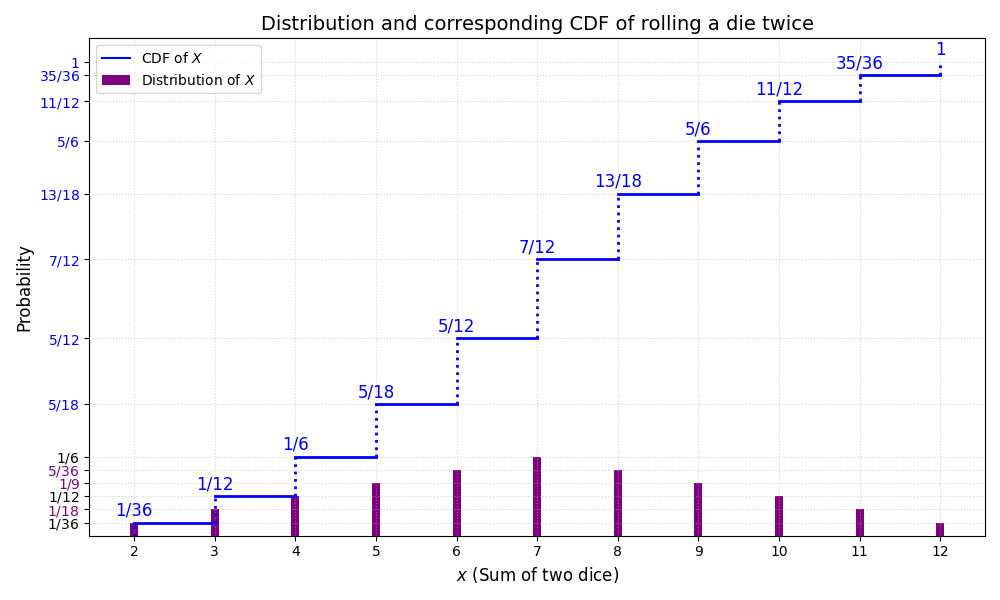
\includegraphics[scale=0.45]{chapter-1/sections/img}
            \caption{Two different characteristics of the random variable $X$ defined by the sum of two dice.\label{fig:figure-distribution-random-variable}}
        \end{figure}
        \item \textbf{Rolling a die until we get 6:} In this case, the random variable $X$ takes values in $\mathbb{N} \cup \{\infty\}$. The distribution of $X$ is given by
        \[
            P_X(\{n\})  = \mathbb{P}(\{\omega \in \Omega \mid X(\omega) = n\}) = \frac{5^{n-1}}{6^n} \quad \text{for } n \in \mathbb{N},
        \]
        However, in this case $F_X$ is
        \[
            \begin{aligned}
                F_X(n) &= P(\{\omega \in \Omega \mid  X(w) \leq n \}) \\
                &= P_X(\{1, \dots, n\}) \\
                &= \sum_{k=1}^n P_X(\{k\}) \\
                &= \sum_{k=1}^n \frac{5^{k-1}}{6^k} = 1 - \frac{5^n}{6^n}.
            \end{aligned}
        \]
        The visualisation of distribution and CDF of this random variable is shown in Figure~\ref{fig:figure-distribution-random-variable-2}.
        \begin{figure}[h]
            \centering
            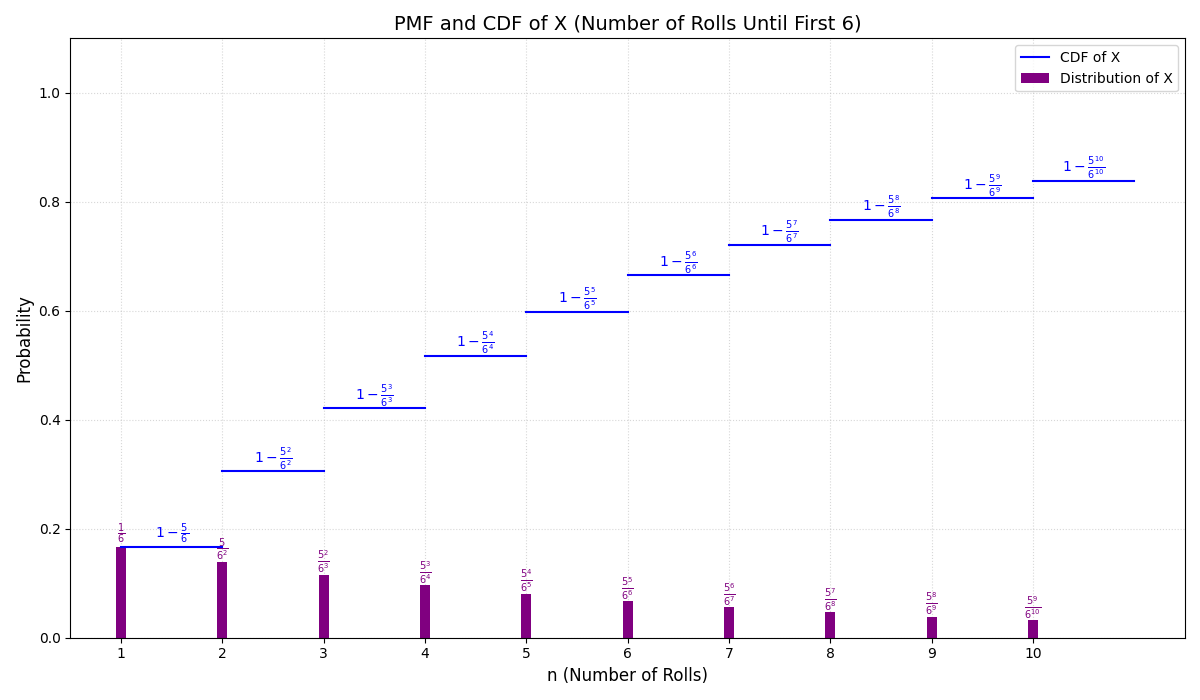
\includegraphics[scale=0.35]{chapter-1/sections/img_1}
            \caption{Two different characteristics of the random variable $X$ defined by the amount of rolls until we get $6$.\label{fig:figure-distribution-random-variable-2}}
        \end{figure}
    \end{itemize}
\end{example}

Certain distributions appear so frequently in theory and applications that they are given special names. These distributions can be \emph{discrete}, where the random variable takes values in a countable set, or \emph{continuous}.

\begin{example}[Classical Distributions]
    \label{ex:classical-distributions}
    Below are two foundational examples of discrete distributions.

    \begin{itemize}
        \item \textbf{The Uniform Distribution.} Let $(\Omega, \mathcal{F}, \mathbb{P})$ be a probability space and  $X: \Omega \to \mathbb{R}$ be a random variable that takes finitely many distinct values, say $\{a_1, \dots, a_n\} \subseteq \mathbb{R}$. We say $X$ has a uniform distribution if each outcome is equally likely. The probability is given by:
        \[
            P_X(\{a_i\}) = \frac{1}{n}, \quad \forall a_i \in \{a_1, \dots, a_n\} \subseteq \mathbb{R}.
        \]
        A random variable that returns the value on upper face of a fair six-sided die roll is an example of uniformly distributed random variable where $X(\omega) \in \{1, 2, 3, 4, 5, 6\}$ and each outcome is equally likely.

        \item \textbf{The Bernoulli Distribution.} This is the distribution of a random variable $X$ with values in $\{0, 1\}$, governed by a parameter $p \in [0, 1]$:
        \[
            P_X(\{1\}) = p \quad \text{and} \quad P_X(\{0\}) = 1 - p.
        \]
        This distribution models a single trial with two possible outcomes, often interpreted as "success" (1) and "failure" (0), such as a single toss of a potentially biased coin.
    \end{itemize}
\end{example}

It is worth noting that these definitions can overlap. A random variable representing a single fair coin toss (e.g., mapping heads to 1 and tails to 0) follows a Bernoulli distribution with parameter $p=1/2$. At the same time, it also follows the uniform distribution on the finite set $E=\{0, 1\}$, since each outcome has probability $1/|E| = 1/2$.

\subsection{Expected value of a random variable}

The final core concept is the expectation, which formalizes the intuitive idea of the 'average' or 'mean' value of a random variable. For a variable that takes on a finite set of values, its expectation is computed as a weighted average, with the probabilities serving as weights. When a random variable takes on a continuous range of values, this weighted average is calculated via integration. In the definition below, we denote the absolute value of a random variable $X$ by $|X|$.

\begin{definition}[Expected Value]
    Let $X$ be a random variable on a probability space $(\Omega, \mathcal{F}, \mathbb{P})$. The \emph{expected value} (or \emph{expectation}) of $X$, denoted $E[X]$, is its integral with respect to the probability measure $P$:
    \[
        E[X] \coloneq \int_{\Omega} X(\omega) \, d\mathbb{P}(\omega).
    \]
    The expectation is said to exist if this integral is well-defined (specifically, if $E[|X|] < \infty$).
\end{definition}

The well-definedness condition of the expectation integral is crucial and is discussed in detail in \cite[Chap 8]{MeasureTheoryLeGall}. It's outside the scope of this dissertation to delve into the intricacies of this condition, but we will provide a brief overview of how the expectation is constructed for random variables.

\begin{example}
    Following the setup in~\ref{ex:indicator-function-in-probability}, consider the indicator function $\mathds{1}_A: \Omega \to \mathbb{R}$ for an event $A$. The expectation of an indicator function is simply the probability of the event it represents:
    \[
        E[\mathds{1}_A] = \mathbb{P}(A) \times 1 + \mathbb{P}(X \setminus A) \times 0 = \mathbb{P}(A).
    \]
\end{example}

From these, we can construct random variables that take a finite number of values.

\begin{definition}[Simple Random Variable]
    Let $(\Sigma, \mathcal{F}, P)$ be a probability space. A random variable $X: \Sigma \to \mathbb{R}$ is called a \emph{simple random variable} if it can be written as a finite linear combination of indicator functions:
    \[
        X = \sum_{i=1}^n a_i \mathds{1}_{A_i},
    \]
    where $a_i \in \mathbb{R}$ are the distinct values taken by $X$ and $A_i = X^{-1}(\{a_i\})$ are the corresponding disjoint events.
\end{definition}

It's important to note that if $X$ is such simple random variable taking finitely many values $\{a_1, \dots, a_n\} \subseteq \mathbb{R}$, then
\[
    \begin{aligned}
        \Omega &= X^{-1}(\{a_1\}) \cup X^{-1}(\{a_2\}) \cup \dots \cup X^{-1}(\{a_n\}) \\
        &= A_1 \cup A_2 \cup \dots \cup A_n,
    \end{aligned}
\]
Hence, we can use the linearity of $X$ to compute the expectation of a simple random variable:
\[
    E[X] = \sum_{i=1}^n a_i E[\mathds{1}_{A_i}] = \sum_{i=1}^n a_i \mathbb{P}(A_i).
\]

%The formal construction of the expectation integral then proceeds as follows:
%\begin{enumerate}
%    \item For a \textbf{simple random variable} $X = \sum_{i=1}^n a_i \mathbf{1}_{A_i}$, the expectation is defined as the weighted average:
%    \[
%        E[X] = \sum_{i=1}^n a_i P(A_i).
%    \]
%    \item For a \textbf{non-negative random variable} ($X \geq 0$), the expectation is defined by approximating $X$ from below with simple random variables:
%    \[
%        E[X] = \sup \{ E[Y] \mid Y \text{ is simple and } 0 \leq Y \leq X \}.
%    \]
%    \item For a \textbf{general random variable}, we decompose it into its positive and negative parts, $X = X^+ - X^-$, where $X^+ = \max(X, 0)$ and $X^- = \max(-X, 0)$. The expectation is then:
%    \[
%        E[X] = E[X^+] - E[X^-],
%    \]
%    provided that at least one of the terms on the right is finite.
%\end{enumerate}

\begin{example}
    Let's apply this definition to our running examples.
    \begin{itemize}
        \item \textbf{Rolling a die twice:} The random variable $X$, representing the sum of the outcomes, is a simple random variable taking values in $\{2, 3, \dots, 12\}$. We can directly apply the formula from step 1:
        \[
            E[X] = \sum_{k=2}^{12} k \cdot P_X(\{k\}).
        \]
        Calculating the probabilities for each sum (e.g., $\mathbb{P}(\{2\})=1/36$, $\mathbb{P}(\{3\})=2/36$, etc.), we find:
        \[
            \begin{aligned}
                E[X] &= 2 \cdot P_X(\{2\}) + 3 \cdot P_X(\{3\}) + \dots + 12 \cdot P_X(\{12\}) \\
                &= 2 \cdot \frac{1}{36} + 3 \cdot \frac{2}{36} + \dots + 12 \cdot \frac{1}{36} = 7\\
            \end{aligned}
        \]
        \item \textbf{Rolling a die until we get 6:} The random variable $X$, representing the number of rolls, is a non-negative but not simple random variable. Its expectation is found using the definition for non-negative variables, which for a discrete variable taking values in $\mathbb{N}$ simplifies to the infinite sum:
        \[
            \begin{aligned}
                E[X] &= \sum_{n=1}^{\infty} n \cdot P_X(\{n\}) \\
                &= \sum_{n=1}^{\infty} n \cdot \frac{5^{n-1}}{6^n} = \frac{1}{6} \sum_{n=1}^{\infty} n \left(\frac{5}{6}\right)^{n-1} \\
                &= \frac{1}{6} \cdot \frac{1}{(1 - 5/6)^2} = \frac{1}{6} \cdot 36
            \end{aligned}
        \]
        This means we expect to wait 6 rolls on average to see the first 6.
    \end{itemize}
\end{example}

%\begin{example}[Continuous Random Variable]
%    When a random variable's distribution is described by a \emph{probability density function} (pdf) $f_X(x)$, the abstract expectation integral simplifies to a more familiar Riemann-style integral. For a random variable $X$ following the Uniform distribution on $[0, 1]$, the pdf is $f_X(x) = 1$ for $x \in [0, 1]$ and 0 otherwise. The expectation is:
%    \[
%        E[X] = \int_{-\infty}^{\infty} x f_X(x) \, dx = \int_0^1 x \cdot 1 \, dx = \left[ \frac{x^2}{2} \right]_0^1 = \frac{1}{2}.
%    \]
%    This confirms the intuition that the average value of a number chosen uniformly from the interval $[0, 1]$ is its midpoint.
%\end{example}
%\section{Probability space}

We denote by $\Omega$ the set of all possible outcomes of a probabilistic experiment, called a \emph{sample space}.

\begin{definition}[Random variable]
    A \emph{random variable} $X$ is a function from the sample $\Omega$ to the set of real numbers $\mathbb{R}$:
    \[
        X: \Omega \to \mathbb{R}
    \]
    \begin{itemize}
        \item The real number $X(w) \in \mathbb{R}$ associated to a sample point $w \in \Omega$ is called a \emph{realization} of the random variable.
        \item The set of all possible realizations $\{X(w) \mid w \in \Omega\} \subseteq \mathbb{R}$ is called \emph{support} and is denoted by $\mathbb{R}_X$.
    \end{itemize}
\end{definition}

\begin{example}[Coin flip]
    $\Omega = \{T, H\}$ and $P(T) = P(H) = \frac{1}{2}$

    $X: \Omega \to \mathbb{R}$ is defined as follows
    \[
        X(w) = \left\{
                   \begin{aligned}
                       1  \quad &\textrm{  if } w = T \\
                       -1  \quad &\textrm{  if } w = H \\
                   \end{aligned}
        \right
    \]

    Then
    \[
        \begin{aligned}
            P(X = 1) &= P(\{w \in \Omega: X(w) = 1\}) = \frac{1}{2} \\
            P(X = -1) &= P(\{w \in \Omega: X(w) = -1\}) = \frac{1}{2} \\
            P(X = 2) &= P(\{w \in \Omega: X(w) = 2\}) = 0 \\
        \end{aligned}
    \]
\end{example}

\begin{notenl}[Notation]
    We usually write $X$ instead of $X(w)$. If $A \subseteq \mathbb{R}$, we write
    \[
        P_X(A) = P(X \in A) = P(\{w \in \Omega: X(w) \in A\})
    \]
\end{notenl}

\subsection{Discrete and Continuous random variables}
%https://www.statlect.com/fundamentals-of-probability/random-variables#rigor
\begin{definition}[Discrete Random Variable]
    A random variable $X$ is \emph{discrete} if
    \begin{enumerate}
        \item its support $\mathbb{R}_X$ is a countable set
        \item there is a \emph{probability mass function}  $p_X: \mathbb{R} \to [0, 1]$ (PMF or probability function) of $X$ such that for any $y \in \mathbb{R}$
        \[
            p_X(y) = \left\{
            \begin{aligned}
                &P(X = y) &\text{ if } y \in \mathbb{R}_X\\
                &0 &\text{ if } y \not \in \mathbb{R}_X\\
            \end{aligned}
        \]

    \end{enumerate}
\end{definition}

\begin{example}[Bernoulli random variable]
    A Bernoulli random variable $X$ is a discrete random variable that takes two values
    \begin{itemize}
        \item it takes $1$ with probability $q$
        \item it takes $0$ with probability $1 - q$
    \end{itemize}
    where $0 \leq q \leq 1$. So the support of this random variable is $\mathbb{R}_X = \{0, 1\}$ and its probability mass function is
    \[
        \[
            p_X(y) = \left\{
            \begin{aligned}
                &q &\text{ if } y = 1\\
                &1-q &\text{ if } y = 0\\
                &0 &\text{ otherwise }\\
            \end{aligned}
        \]
    \]
\end{example}

\begin{notenl}[Properties of probability mass function]
    PMF is characterised by two fundamental properties:
    \begin{itemize}
        \item \textbf{Non-negativity}: $p_X(x) \geq 0$ for any $x \in \mathbb{R}$.
        \item \textbf{Total sum is 1}: $\sum_{x \in \mathbb{R}_X}p_X(x) = 1$.
    \end{itemize}

    Any PMF satisfies these two properties and any function satisfying these properties is legitimate PMF.
\end{notenl}

\begin{definition}[Continuous random variables]
    A random variable $X$ is \emph{continuous} if
    \begin{itemize}
        \item its support $\mathbb{R}_X$ is an uncountable set
        \item there is a \emph{probability density function} $f_X: \mathbb{R} \to [0, \infty)$ (PDF or density function) of $X$ such that for any interval $[a, b] \subset \mathbb{R}$
        \[
            P(X \in [a, b]) = \int_{a}^{b} f_X(x)dx
        \]
    \end{itemize}
\end{definition}

\begin{example}[Uniform random variable]
    A uniform random variable $X$ (on the interval $[0, 1]$) is a continuous variable that can take any value in the interval $[0, 1]$ (i.e $\mathbb{R}_X = [0, 1]$). Its probability density function is
    \[
        f_X(x) = \left\{
                     \begin{aligned}
                         &1 &\text{ if } x \in [0, 1]\\
                         &0 &\text{ otherwise }
                     \end{aligned}
        \right.
    \]

    Probability that the realization of $X$ belongs to $[\frac{1}{4}, \frac{3}{4}]$ is
    \[
        \begin{aligned}
            P(X \in [\frac{1}{4}, \frac{3}{4}]) &= \int_{\frac{1}{4}}^{\frac{3}{4}} f_X(x)dx \\
            &= \int_{\frac{1}{4}}^{\frac{3}{4}} 1 dx \\
            &= \left[ x \right]_{\frac{1}{4}}^{\frac{3}{4}} \\
            &= \frac{3}{4} - \frac{1}{4} = \frac{1}{2}.
        \end{aligned}
    \]
\end{example}

\begin{notenl}[Properties of probability density function]
    PDF is characterised by two fundamental properties:
    \begin{itemize}
        \item \textbf{Non-negativity}: $f_X(x) \geq 0$ for any $x \in \mathbb{R}$.
        \item \textbf{Total integral is 1}: $\int_{-\infty}^{+\infty} f_X(x)dx = 1$.
    \end{itemize}

    Any PDF satisfies these two properties and any function satisfying these properties is legitimate PDF.
\end{notenl}

\begin{definition}[Probability measure]
    Let $\Omega$ be a sample space and $\mathcal{F}$ be space of events, i.e. a $\sigma$-algebra on $\Omega$. We say that $P: \mathcal{F} \to [0, 1] $ is a \emph{probability measure} if it satisfies the following properties:
    \begin{enumerate}[label=(\roman*)]
        \item $P(\emptyset) = 0$,
        \item $P(\Omega) = 1$,
        \item If $E_1, E_2, \dots$ are pairwise disjoint sets in $\mathcal{F}$, then
        \[
            P\left(\bigcup_{i=1}^\infty E_i\right) = \sum_{i=1}^\infty P(E_i).
        \]
    \end{enumerate}
\end{definition}

\subsection{Expected value}
%https://www.stat.auckland.ac.nz/~fewster/325/notes/ch3.pdf

\begin{definition}[Expected value]
    The definition of the expected value of a random variable $X$ depends on whether $X$ is discrete or continuous.
    \begin{itemize}
        \item If $X$ is discrete, then the expected value of $X$ is defined as
        \[
            \mathbb{E}[X] = \sum_{x \in \mathbb{R}_X} x \cdot p_X(x)
        \]
        where $p_X(x)$ is the probability mass function of $X$.

        \item If $X$ is continuous, then the expected value of $X$ is defined as
        \[
            \mathbb{E}[X] = \int_{-\infty}^{+\infty} x f_X(x)dx
        \]
        where $f_X(x)$ is the probability density function of $X$.
    \end{itemize}
\end{definition}

\subsection{Probability distribution function}
%https://math.arizona.edu/~jwatkins/G_randomvariables.pdf
Having a random variable of interest $X$, the question typically becomes "What is the probability that $X$ takes a value in a certain range?" To answer this, we need to define the distribution function of the random variable.

\begin{definition}[Distribution function]
    The $X$ be a random variable. The \emph{distribution function} (or cumulative distribution function, CDF) of $X$ is defined as
    \[
        F_X(x) = P(X \leq x) = P(\{w \in \Omega: X(w) \leq x\})
    \]
    for all $x \in \mathbb{R}$.
\end{definition}

By knowing the distribution function $F_X(x)$, we can find the probability of $X$ being in an interval $[a, b]$:
\begin{equation}
    \label{eq:probability-interval}
    P(X \in [a, b]) = F_X(b) - F_X(a)
\end{equation}
%\input{chapter-2/model-theory}

    \chapter{Non-Independence Property of O-minimal structures}\label{ch:nip-property}

We follow the presentation of~\cite[Chap.~5]{vandenDries1998} to develop a general combinatorial framework that will later be applied to o-minimal structures. The central aim is to show that every definable family in an o-minimal structure satisfies a strong restriction on the number of distinct subsets it can induce on finite sets: there exists a fixed exponent $d$ such that, for all sufficiently large finite sets $F$, the number of subsets of $F$ "shattered" by the family grows at most like $|F|^{d}$, rather than exponentially. Most of the chapter proceeds in a general setting, introducing the basic combinatorial notions of families of subsets and their growth functions, and proving a sharp dichotomy—either the family generates exponentially many subsets, or its growth is bounded by a polynomial. A key tool is the duality between a family of sets and its parameter space, allowing us to transfer growth bounds between the two. This dual perspective connects naturally to a model-theoretic tameness condition, the non-independence property (NIP). In the final part, we specialise these general results to the o-minimal setting and prove that every definable family is NIP. Beyond its intrinsic interest, this fact will serve as a crucial ingredient in the learning-theoretic framework developed in a later chapter.



\section{Combinatorial Preliminaries and Growth Function}

In this section we are going to introduce the basic combinatorial tools that provides the basis for our discussion including the concept of shattering, growth function of a family of subsets. The main aim of this section is to prove a theorem, which is referred as combomatorial dichotomy that characterises the growth function of a family of subsets.

\subsection{Shattering}

We begin with a purely combinatorial setup. Fix an infinite set $X$ and a collection of its subsets, $\mathcal{C} \subseteq \mathcal{P}(X)$. For any finite set $F\subseteq X$, we are interested in the subsets of $F$ that can be \emph{cut out} by the sets in $\mathcal{C}$. This is called the \emph{trace} of $\mathcal{C}$ on $F$.
\[
    \mathcal{C}\cap F=\{C\cap F:C\in\mathcal{C}\}.
\]
Since $F$ is finite, it has $2^n$ subsets, ie $|\mathcal{P}(F)| = 2^n$. If all of the subsets of $F$ can be cut out by $\mathcal{C}$, we say \emph{$\mathcal{C}$ shatters $F$}. We define this more formally below.

\begin{definition}[Shattering]
    Let $\mathcal{C} \subseteq \mathcal{P}(X)$. We say that $\mathcal{C}$ \emph{shatters} a finite set $F \subseteq X$ if the trace of $\mathcal{C}$ on $F$ is the entire power set of $F$. That is, if $\mathcal{C} \cap F = \mathcal{P}(F)$, or equivalently, $|\mathcal{C} \cap F| = 2^{|F|}$.
\end{definition}

Note that, shattering is the key concept that underlying the combinatorial dichotomy we will introduce below. It's also important to emphasize that, generally speaking, we are not interested in $\mathcal{C}$ shattering any specific finite subset, rather we want to know given $n\in \mathbb{N}$, can $\mathcal{C}$ shatter some finite set of size $n$. If the answer is "no" for given $n$, then we want to know what is the maximum number of subsets $\mathcal{C}$ can cut out from a finite set of size $n$. To measure this \textit{combinatorial complexity} of $\mathcal{C}$, we define its \emph{growth function}, which measures the maximum size of a trace on any set of size $n$.
\begin{equation}\label{eq:growth-func-def-1}
f_{\mathcal{C}}(n)\coloneq\max\bigl\{|\mathcal{C}\cap F|:F\subseteq X,\ |F|=n\bigr\}.
\end{equation}
Note that, we always have $f_{\mathcal{C}}(n) \le 2^n$. Following theorem states that the combinatorial complexity of $\mathcal{C}$, which is determined by its growth function, can only be polynomial or exponential.

\begin{theorem}[Combinatorial Dichotomy]
    \label{thm:vc-dichotomy}
    Let $X$ and $\mathcal{C}$ be given as above. Then exactly one of the following holds:
    \begin{enumerate}[label=(\roman*)]
        \item $f_{\mathcal{C}}(n)=2^{n}$ for every $n\in\mathbb{N}$.
        \item There exists an integer $d\ge 1$ such that
        \[
            f_{\mathcal{C}}(n)\le n^d
        \]
        for all sufficiently large $n \in \mathbb{N}$.
    \end{enumerate}
\end{theorem}

\begin{remark}
    In the first case of~\ref{thm:vc-dichotomy}, we say that $\mathcal{C}$ has \emph{exponential growth}. In the second case, we say that $\mathcal{C}$ has \emph{polynomial growth} and we call $d$ the \emph{degree} of the polynomial bound. The dichotomy is a powerful tool in combinatorial geometry and model theory, as it allows us to classify families of sets based on their growth behavior.

    We will prove this theorem using the following lemma.
\end{remark}
\subsection{Proof of the combinatorial dichotomy}

In this subsection we will prove the theorem~\ref{thm:vc-dichotomy}. We need following lemma to establish the desired result.

\begin{lemma}
    \label{lem:combinatorial-lemma}
    Let $F$ be a finite set with $|F|=n$ and $\mathcal{D} \subseteq \mathcal{P}(F)$ such that
    \begin{equation}
        \label{eq:assumption-combinatorial-lemma}
        |\mathcal{D}| > \sum_{i=0}^{d-1}\binom{n}{i}
    \end{equation}
    where $0 \leq d \leq n$. Then $F$ has a subset $E$ such that $|E|=d$ and $\mathcal{D}$ shatters $E$.
\end{lemma}

\begin{remark}

    To see why the the inequality is strict, consider the collection $\mathcal{D}^*$ consisting of all subsets of $F$ of size strictly less than $d$. The cardinality of this collection is exactly the sum on the right-hand side:
    \[
        |\mathcal{D}^*| = \sum_{i=0}^{d-1}\binom{n}{i}.
    \]
    This collection $\mathcal{D}^*$ fails to satisfy the lemma's conclusion. For any subset $E \subseteq F$ of size $d$, the trace $\mathcal{D}^* \cap E$ cannot equal $\mathcal{P}(E)$. This is because the set $E$ itself, which is an element of $\mathcal{P}(E)$, has size $d$. However, every set in $\mathcal{D}^*$ has size less than $d$, so no intersection with $E$ can possibly recover $E$ itself. This demonstrates that the strict inequality in the lemma's hypothesis is essential.

    The significance of this bound extends beyond its role as a sharp threshold. Let us denote the sum of binomial coefficients as a function of $n$:
    \begin{equation}
        \label{eq:def-pascal-identity}
        p_d(n) \coloneq \sum_{i=0}^{d-1}\binom{n}{i}.
    \end{equation}
    The function $p_d(n)$ itself exhibits a remarkable regularity, which can be understood in two key ways.

    Firstly, for a fixed integer $d$, the expression $p_d(n)$ is a \textit{polynomial in $n$} with rational coefficients of degree $d-1$. This is because each term $\binom{n}{i} = \frac{n(n-1)\dots(n-i+1)}{i!}$ is a polynomial in $n$ of degree $i$. The degree of the sum is therefore determined by the highest-degree term, which is $\binom{n}{d-1}$. This algebraic property allows us to analyze the bound using tools from algebra, even extending its definition from integer inputs $n$ to real numbers $x$.

    Secondly, this polynomial satisfies a \textit{recursive relationship} that mirrors the famous Pascal's identity. By summing the identity $\binom{n}{k} = \binom{n-1}{k} + \binom{n-1}{k-1}$ over $k$, one can derive the following \texit{Pascal triangle equality} for the polynomials:
    \begin{equation}
        \label{eq:pascal-identity}
        p_d(n) = p_d(n-1) + p_{d-1}(n-1).
    \end{equation}

    This identity reveals an orderly, systematic way in which the bound grows, connecting its value for a set of size $n$ to its values for a smaller set. We will use this in the proof of the lemma~\ref{lem:combinatorial-lemma}.

\end{remark}

\begin{proof}[Proof of~\ref{lem:combinatorial-lemma}]

    We will prove the lemma by induction on $n$. If $d=0$, the only subset of $F$ is the empty set, and the trace $\mathcal{D} \cap F$ is trivially $\{\emptyset\}$, which is equal to $\mathcal{P}(\emptyset)$. Thus, the lemma holds. On the other hand, $d = n$, then $\mathcal{D}$ must contain all subsets of $F$, which is $\mathcal{P}(F)$. The trace $\mathcal{D} \cap F$ is then equal to $\mathcal{P}(F)$, satisfying the lemma.

    Assume $0 < d < n$. We pick an arbitrary point $x \in F$ and write
    \[
        F' \coloneq F \setminus \{x\} \textrm{ and } \mathcal{D}' \coloneq \{D \cap F' \mid D \in \mathcal{D}\}
    \]
    Let $\phi: \mathcal{D} \to \mathcal{D}'$ be the surjective function that maps each set in $\mathcal{D}$ to its intersection with $F'$, that is $\phi(D) = D \cap F'$. Note that for each $D \in \mathcal{D}$, there are two possibilities:
    \[
        D \cap F' = D \text{ if } x \notin D  \textrm{  or  }  D \cap F' = (D \setminus \{x\}) \text{ if } x \in D.
    \]
    So, for a given $D' \in \mathcal{D'}$, we have
    \[
        |\phi^{-1}(D')| = \begin{cases}
                              1 & \text{if } D' \cup \{x\} \notin \mathcal{D} \textrm{ or } D' \notin \mathcal{D} \\
                              2 & \text{if } D' \cup \{x\} \in \mathcal{D} \textrm{ and } D' \in \mathcal{D}
        \end{cases}
    \]
    Hence, we can partition $\mathcal{D}'$ into two parts: $\mathcal{D}' = \mathcal{D}_1 \cup \mathcal{D}_2$, where $\mathcal{D}_1$ contains the sets of $\mathcal{D}'$ that has only one preimage under $\phi$ and $\mathcal{D}_2$ contains the sets that have two preimages.
    Recall,~\ref{eq:def-pascal-identity}. There are two cases to consider:
    \begin{enumerate}[label=(\roman*)]
        \item $|\mathcal{D}'| > p_d(n-1)$. Then by the induction assumption applied to $F'$ and $\mathcal{D}'$, there is a subset $E \subseteq F$ of size $d$ with $\mathcal{D}' \cap E = \mathcal{P}(E)$. Since $\mathcal{D} \cap E = \mathcal{D}' \cap E$ by definition of $\mathcal{D}'$, we have $\mathcal{D} \cap E = \mathcal{P}(E)$, which satisfies the lemma.
        \item $|\mathcal{D}'| \leq p_d(n-1)$. Then, we have,
        \[
            \begin{aligned}
                |\mathcal{D}| &= |\mathcal{D}_1| + 2|\mathcal{D}_2| \\
                &= |\mathcal{D}'| + |\mathcal{D}_2| \textrm{ (since $\mathcal{D}'$ is disjoint union of $\mathcal{D}_1$ and $\mathcal{D}_2$)} \\
                &> p_d(n) \textrm{ (by the lemma's assumption~\ref{eq:assumption-combinatorial-lemma})} \\
                &= p_d(n-1) + p_{d-1}(n-1) \textrm{ (by the Pascal Identity~\ref{eq:pascal-identity})} \\
            \end{aligned}
        \]
        So it follows that $|\mathcal{D}_2| > p_{d-1}(n-1)$. By the induction assumption applied to $F'$ and $\mathcal{D}_2$, there is a subset $E \subseteq F'$ of size $d-1$ with $\mathcal{D}_2 \cap E = \mathcal{P}(E)$. To derive $\mathcal{D} \cap (E \cup \{x\}) = \mathcal{P}(E \cup \{x\})$, let $E' \coloneq E \cup \{x\}$, which has size $d$. Take any subset $A \subseteq E'$.
        If $x \notin A$, then $A \subseteq E$. Since $\mathcal{D}_2$ shatters $E$, there is some $S \in \mathcal{D}_2$ such that $S \cap E = A$. By definition of $\mathcal{D}_2$, $S \in \mathcal{D}$, and since $x \notin S$, we have $S \cap E' = A$.

        If $x \in A$, let $A_0 = A \setminus \{x\}$. Since $A_0 \subseteq E$, there is some $S_0 \in \mathcal{D}_2$ such that $S_0 \cap E = A_0$. By definition of $\mathcal{D}_2$, the set $S_0 \cup \{x\}$ is in $\mathcal{D}$, and its trace on $E'$ is $(S_0 \cup \{x\}) \cap E' = (S_0 \cap E) \cup \{x\} = A_0 \cup \{x\} = A$.

        Since all subsets of $E'$ can be formed, $\mathcal{D} \cap E' = \mathcal{P}(E')$, which completes the proof.
    \end{enumerate}
\end{proof}

\begin{example}
    Let $F$ be a set of size $n=4$ and let $d=3$. The bound from the lemma is:
    \[
        p_3(4) = \binom{4}{0} + \binom{4}{1} + \binom{4}{2} = 1 + 4 + 6 = 11.
    \]
    The lemma asserts that any collection $\mathcal{D}$ of more than 11 subsets of $F$ must shatter some 3-element subset. The sharpness is confirmed by the collection of all subsets of size less than 3, which has exactly 11 elements and fails to shatter any 3-element set. We can also verify the recursive identity:
    \begin{itemize}
        \item $p_3(3) = \binom{3}{0} + \binom{3}{1} + \binom{3}{2} = 1 + 3 + 3 = 7$.
        \item $p_2(3) = \binom{3}{0} + \binom{3}{1} = 1 + 3 = 4$.
        \item Indeed, $p_3(4) = 11 = 7 + 4 = p_3(3) + p_2(3)$.
    \end{itemize}
\end{example}

We know prove the theorem~\ref{thm:vc-dichotomy} using the lemma~\ref{lem:combinatorial-lemma}.

\begin{proof}[Proof of Theorem~\ref{thm:vc-dichotomy}]

    The cases are clearly mutually exclusive: if $f_{\mathcal{C}}(n) = 2^n$ for all $n$, its exponential growth cannot be bounded by any polynomial $n^d$ for all sufficiently large $n$. The core of the proof is to show that if case (i) does not hold, then case (ii) must hold.

    Suppose, there exists an integer $d \ge 1$ such that $f_{\mathcal{C}}(d) < 2^d$. Without loss of generality, we can assume $d$ is the smallest integer for which this holds. By definition, this means that for all $k < d$, $f_{\mathcal{C}}(n) = 2^k$.

    Fix $n \geq d$ and let $F$ be a finite subset of $X$ with $|F| = n$. Then $p_d(n)$ is a polynomial in $n$ of degree $d-1$. If $|\mathcal{C} \cap F| > p_d(n)$, then by the lemma~\ref{lem:combinatorial-lemma}, there exists a subset $E \subseteq F$ of size $d$ such that $\mathcal{C} \cap E = \mathcal{P}(E)$. This means that $\mathcal{C}$ shatters the set $E$, which contradicts our assumption that $f_{\mathcal{C}}(d) < 2^d$. Hence, we must have $|\mathcal{C} \cap F| \leq p_d(n)$ for all $n \geq d$. Since $F$ was arbitrary, this implies that
    \[
        f_{\mathcal{C}}(n) \leq p_d(n) \leq n^d
    \]
    for all sufficiently large $n$. This establishes case (ii) of the theorem.


\end{proof}

Following corollary is equivalent to the theorem~\ref{thm:vc-dichotomy} and is often used in practice.

\begin{corollary}
    \label{cor:vc-dichotomy}
    Suppose $f_{\mathcal{C}}(d) < 2^d$ for some integer $d \ge 1$. Then $f_{\mathcal{C}} \leq p_d(n)$ for all $n \in \mathbb{N}$.
\end{corollary}
\section{Non-independence property}

In this section, we build on the notions introduced earlier—specifically, \textit{shattering} and the \textit{growth function}—to formalise the Non-Independence Property (NIP) for families of sets. Our exposition follows~\cite[Chap.~5]{vandenDries1998}. We begin by defining the Vapnik–Chervonenkis (VC) dimension of a family of sets in terms of shattering. We then show that, when the VC-dimension is finite, this property admits an equivalent characterisation via a model-theoretic notion of \textit{dependence}. These dual perspectives on finite VC-dimension will serve as the foundation for the main result of this section: informally, that if a collection of subsets is dependent in lower dimensions, then this dependence persists in higher dimensions.

\subsection{VC-Classes and VC-Dimension}

\begin{definition}[VC-Class and VC-Dimension]\label{def:vc-class-dimension}
    A collection $\mathcal{C} \subseteq \mathcal{P}(X)$ is called a \emph{Vapnik-Chervonenkis class} (or \emph{VC-class}) if there exists some $d \in \mathbb{N}$ such that $\mathcal{C}$ does not shatter any set of size $d$. The \emph{VC-dimension} of $\mathcal{C}$, denoted $V(\mathcal{C})$, is defined as:
    \[
        V(\mathcal{C}) \coloneq \min \{|F| : F \subseteq X \text{ is finite and is not shattered by } \mathcal{C}\}.
    \]
    If $\mathcal{C}$ is a VC-class, then $V(\mathcal{C})$ is the size of the largest finite set shattered by $\mathcal{C}$. If $\mathcal{C}$ is not a VC-class (i.e., it shatters finite sets of arbitrarily large size), we set $V(\mathcal{C}) = \infty$.
\end{definition}

Thus, a collection $\mathcal{C}$ is a VC-class if and only if its VC-dimension is finite. The dichotomy theorem states that $V(\mathcal{C}) < \infty$ if and only if $f_{\mathcal{C}}:\mathbb{N} \to \mathbb{N}$ has polynomial growth, while $V(\mathcal{C}) = \infty$ if and only if $f_{\mathcal{C}}(n) = 2^n$ for all $n$.

\begin{example}[Intervals]
    Let $X = \mathbb{R}$ and let $\mathcal{C}$ be the collection of all closed intervals $[a, b]$.
    \begin{itemize}
        \item $\mathcal{C}$ shatters the set $F_1 = \{5\}$. The trace is $\{\emptyset, \{5\}\}$ (using intervals like $[0,1]$ and $[4,6]$).
        \item $\mathcal{C}$ shatters the set $F_2 = \{5, 10\}$. To get all four subsets:
        \begin{itemize}
            \item $\emptyset$: use $[0,1]$
            \item $\{5\}$: use $[4,6]$
            \item $\{10\}$: use $[9,11]$
            \item $\{5, 10\}$: use $[4,11]$
        \end{itemize}
        \item $\mathcal{C}$ does \emph{not} shatter $F_3 = \{5, 10, 15\}$. It is impossible to find an interval that contains $\{5, 15\}$ but not $\{10\}$.
    \end{itemize}
    The largest set shattered has size 2, so $V(\mathcal{C}) = 2$.
\end{example}

\begin{example}[An Infinite VC-Dimension Class]
    \label{ex:vc-infinite-dimension}
    Let $X = \{p \in \mathbb{N} \mid n \textrm{ is prime}\}$ be the given set. Consider the collection of subsets
    \[
        \mathcal{C} = \{C_n : n \in \mathbb{N}\} \textrm{ where } C_n = \{p \in X : p \text{ divides } n\}
    \]
    We claim $V(\mathcal{C}) = \infty$. To prove this, we must show that $\mathcal{C}$ can shatter any finite set of primes $F = \{p_1, p_2, \dots, p_d\}$.

    Let $E = \{q_1, \dots, q_k\}$ be an arbitrary subset of $F$. We need to find an integer $n$ such that $C_n \cap F = E$. The choice is straightforward: let $n = q_1 \cdot q_2 \cdot \dots \cdot q_k$. By construction, every prime in $E$ divides $n$. Furthermore, no prime in $F \setminus E$ can divide $n$, by the fundamental theorem of arithmetic. Thus, $C_n \cap F = E$. Since we can do this for any subset $E \subseteq F$, $\mathcal{C}$ shatters $F$. As $F$ was an arbitrary finite set of primes, $\mathcal{C}$ shatters sets of all sizes, and $V(\mathcal{C}) = \infty$.
\end{example}
\subsection{Dependence property - Dual perspective into finite VC-dimension}

When a collection $\mathcal{C}$ is naturally parametrised by the elements of another set—such as in Example~\ref{ex:vc-infinite-dimension}, where $\mathcal{C}$ was indexed by the natural numbers—its VC-dimension can often be analysed via a corresponding \textit{model-theoretic} property of the parameter space, namely \textit{(non-in)dependence} propery, shortened as \textit{(N)IP}. In particular, the concept of dependence in model theory serves as a dual perspective to finite VC-dimension. We will see that a parametrised family of sets is dependent precisely when it has finite VC-dimension.

To make this correspondence precise, we adopt the following formal framework. Let $X$ and $Y$ be infinite sets, and let $\Phi \subseteq X \times Y$ be a binary relation. For each $x \in X$ and $y \in Y$, define the sets
\[
    \Phi_x = \{y \in Y : (x,y) \in \Phi\} \subseteq Y \quad \text{and} \quad \Phi^y = \{x \in X : (x,y) \in \Phi\} \subseteq X.
\]

\noindent
Then we define the collections of sets indexed by $Y$ and $X$ correspondingly:
\[
    \mathcal{C}_X = \{\Phi^y : y \in Y\}  \quad \text{and} \quad \mathcal{C}_Y = \{\Phi_x : x \in X\}.
\]
\noindent
Here, $Y$ is the parameter space for $\mathcal{C}_X\subseteq \mathcal{P}(X)$, and $X$ is the parameter space for $\mathcal{C}_Y \subseteq \mathcal{P}(Y)$.

We focus on the trace of $\mathcal{C}_X$ on a finite set $F \subseteq X$. A subset $E \subseteq F$ belongs to the trace $\mathcal{C}_X \cap F$ if and only if there exists some parameter $y \in Y$ such that $E = \Phi_y \cap F$. This condition can be rephrased:
\[
    \begin{aligned}
        E = \Phi_y \cap F \quad &\Leftrightarrow \quad [\forall x \in E, (x,y) \in \Phi] \text{ and } [\forall x \in F \setminus E, (x,y) \notin \Phi] \\
        &\Leftrightarrow \quad [\forall x \in E, y \in \Phi_x] \text{ and } [\forall x \in F \setminus E, y \notin \Phi_x] \\
    \end{aligned}
\]
Therefore,
\begin{equation}
    \label{eq:trace-condition}
    E \in \mathcal{C}_X \cap F \quad \Leftrightarrow \quad \left( \bigcap_{x \in E} \Phi_x \right) \cap \left( \bigcap_{x \in F \setminus E} (Y \setminus \Phi_x) \right) \neq \emptyset. \quad
\end{equation}


Recall that, \emph{atom} is a minimal non-empty set in a Boolean algebra of sets~\cite[Chap 1]{vandenDries1998} in terms of inclusion. If we consider the boolean algebra generated by the sets $\{\Phi_x : x \in F\}$, denoted as $\mathcal{B}(\{\Phi_x : x \in F\})$, the expression on the right-hand side of~\ref{eq:trace-condition} is precisely an atom of this Boolean algebra for each subset $E \in \mathcal{P}(F)$.

Hence, given $\mathcal{C}_X$ and a finite subset $F \subseteq X$ with $|F| = n$, we can use this duality described above to determine if $\mathcal{C}_X$ shatters $F$. More specifically, this can be summarized as follows:
\[
    \begin{aligned}
        \mathcal{C}_X \text{ shatters } F \quad &\Leftrightarrow \quad |\mathcal{C}_X \cap F| = 2^n \\
        &\Leftrightarrow \quad \mathcal{B}(\{\Phi_x : x \in F\}) \text{ has } 2^n \text{ atoms} \\
    \end{aligned}
\]

Note that, here duality emerges from the fact that $\mathcal{C}_X$ is collection of subsets of $X$ indexed by $Y$, while $\{\Phi_x : x \in F\}$ is a collection of subsets of $Y$ indexed by the finite set $F\subset X$. The atoms of the Boolean algebra $\mathcal{B}(\{\Phi_x : x \in F\})$ correspond to the subsets of $F$ that can be isolated by the parameters from $Y$. We will not use this argument based on the atoms of boolean algebra to define a model-theoretic property of $\mathcal{C}_Y$ called \textit{independence}.

Firstly, we need to introduce some notation that will be useful when we use dependence property of a collection of subsets. Let \(Y\) be an arbitrary infinite set, and let \(S \subseteq Y\). We introduce the following notation for any subset \(S\) of \(Y\):
\[
    S^1 \coloneqq S,
    \quad
    S^{-1} \coloneqq Y \setminus S.
\]
\noindent
Next, let \(G = \{1,\dots,n\}\subseteq\mathbb{N}\). For each \(H\subseteq G\), define the sign‐function
\[
    \begin{equation}
        \label{eq:sign-function}
        \mathds{1}_H : G \to \{1,-1\},
        \qquad
        \mathds{1}_H(i) =
        \begin{cases}
            1,  & i\in H,\\
            -1, & i\notin H.
        \end{cases}
    \end{equation}
\]
\noindent
Given subsets \(S_1,\dots,S_n \subseteq Y\) and any \(H\in\mathcal P(G)\), consider the intersection
\[
    S_1^{\mathds{1}_H(1)}
    \,\cap
    S_2^{\mathds{1}_H(2)}
    \,\cap\cdots\cap\,
    S_n^{\mathds{1}_H(n)}.
\]

There are \(2^n\) such intersections; they are pairwise disjoint and their union equals \(Y\). The sequence \((S_1,\dots,S_n)\) exhibits dependence precisely if at least one of these intersections is empty. More precisely, we have the following definition.


\begin{definition}[Independence property]
    Let $Y$ and $S_1, \ldots, S_n \subseteq Y$ be given.
    \begin{itemize}
        \item We say that the sequence $(S_1,  \ldots, S_n)$ is \emph{independent} (in $Y$) if the boolean algebra generated by the sets $S_1, \ldots, S_n$, denoted $\mathcal{B}(S_1, \ldots, S_n)$ has $2^n$ atoms. Otherwise, we say that the sequence is \emph{dependent} (in $Y$).

        \item If a collection $\mathcal{C}_Y \subseteq \mathcal{P}(Y)$ contains independent sequence of size $n$ for every $n \in \mathbb{N}$, we say that $\mathcal{C}_Y$ is \emph{independent} (in $Y$). Otherwise, we say that $\mathcal{C}_Y$ is \emph{dependent} (in $Y$).
    \end{itemize}
\end{definition}

Following proposition is a dual of ~\ref{cor:vc-dichotomy}.

\begin{proposition}{\label{prop:number-of-atoms}}
    Let $\mathcal{C}_Y \subseteq \mathcal{P}(Y)$ be a collection of subsets of an infinite set $Y$. If $\mathcal{C}_Y$ contains no independent sequence of size $d \ge 1$ for some $d$, then for all sequences $S_1, \ldots, S_n \in \mathcal{C}_Y$, the boolean algebra $\mathcal{B}(S_1, \dots, S_n)$ has at most $p_d(n)$ atoms.
\end{proposition}

\begin{proof}

    For $n < d$, $p_d(n) = 2^n$, so $C_Y$ shatters some set of size $n$. Assume, $n \geq d$ and let $S_1, \dots, S_n \in C_Y$. Also, let $F = \{1, \ldots, n\}$ and consider $\mathcal{D} \subseteq \mathcal{P}(F)$ where $\mathcal{D}$ contains subsets $D \subseteq F$ such that
    \[
        S_1^{\mathds{1}_D(1)} \cap S_2^{\mathds{1}_D(2)} \cap \cdots \cap S_n^{\mathds{1}_D(n)} \neq \emptyset.
    \]

    If $|\mathcal{D}| > p_d(n)$, then by the lemma~\ref{lem:dependent-boolean-comb}, there exists a subset $E \subseteq F$ of size $d$ such that $\mathcal{D}$ shatters $E$. Hence, the boolean algebra $\mathcal{B}(S_1, \dots, S_n)$ has $2^d$ atoms, which contradicts the assumption that $\mathcal{C}_Y$ contains no independent sequence of size $d$. Therefore, we must have $|\mathcal{D}| \leq p_d(n)$.
\end{proof}

One of the sufficient conditions for a sequence to be dependent is as follows:
\begin{lemma}{\label{lem:suff-cond-dependencty}}
    Let $\mathcal{C}_Y \subseteq \mathcal{P}(Y)$ be a collection and let $d \in \mathbb{N}$ be such that any non-empty intersection of $d$ sets from $\mathcal{C}_Y$, say $S_1, \dots, S_d \in \mathcal{C}_Y$, is equal to the intersection of at most $d-1$ of those sets $\mathcal{C}_Y$
    \[
        S_1 \cap S_2 \cap \cdots \cap S_d = \bigcap_{i\in D} S_i \quad \text{for some } D \subseteq \{1, 2, \ldots, d\} \text{ with } |D| < d.
    \]
    Then the collection $\mathcal{C}_Y$ is dependent in $Y$.
\end{lemma}

\begin{proof}

    It's enough to show that there is no independent sequence of size $d$ in $\mathcal{C}_Y$. In other words, for an arbitrary sequence $S_1, \dots, S_d$, the number of atoms of the boolean algebra generated by this sequence, $\mathcal{B}(S_1, \dots, S_d)$ is strictly less than $2^d$.

    Let $S_1, \dots, S_d$ be an arbitrary sequence of sets in $\mathcal{C}_Y$. If $S_1 \cap \dots \cap S_d$ is empty then we are done, since this intersection cannot be atom of $\mathcal{B}(S_1, \dots, S_d)$ and this boolean algebra has strictly less than $2^d$ atoms. On the other hand, if $S_1 \cap \dots \cap S_d$ is non-empty, then by assumption
    \begin{equation}
        \label{eq:proof-suff-cont-1}
        S_1 \cap \dots \cap S_d = \bigcap_{i \in D} S_i
    \end{equation}
    for some proper subset $D \subset \{1, \dots, d\}$. It follows that the intersection
    \begin{equation}
        \label{eq:proof-suff-cont-2}
        \begin{aligned}
            \bigl(\bigcap_{i \in D} S_i\bigr) \cap \bigl(\bigcap_{j \not \in D} S^{-1}_j\bigr) =  S_1^{\mathds{1}_D(1)} \cap S_2^{\mathds{1}_D(2)} \cap \cdots \cap S_n^{\mathds{1}_D(n)}\\
        \end{aligned}
    \end{equation}
    is also empty combining~\ref{eq:proof-suff-cont-1} and~\ref{eq:proof-suff-cont-2}, where $\mathds{1}_{D}: \{1, \dots, d\} \to \{-1, 1\}$ is a sign function defined in~\ref{eq:sign-function}. To see this, note that combining~\ref{eq:proof-suff-cont-1} and~\ref{eq:proof-suff-cont-2} we get intersection of two sets that are complement of each other, more precisely,
    \[
        \begin{aligned}
            \bigl(\bigcap_{i \in D} S_i\bigr) \cap \bigl(\bigcap_{j \not \in D} S^{-1}_j\bigr) = S_1 \cap \dots \cap S_d \cap \bigl(\bigcap_{j \not \in D} S^{-1}_j\bigr) = \emptyset.
        \end{aligned}
    \]
\end{proof}

\noindent
We can interpret the lemma~\ref{lem:suff-cond-dependencty} more informally as follows: Let $\mathcal{C}_Y$ and $d$ be as in the statement of the lemma. If we intersect any $d$ sets from $\mathcal{C}_Y$, the result can be expressed as an intersection of fewer than $d$ sets. We will use this lemma to prove the following lemma.

\begin{lemma}
    \label{lem:dependent-boolean-comb}
    Let $\mathcal{C}_Y$ and $d$ be given such that they satisfy the hypothesis of~\ref{lem:suff-cond-dependencty}. Let $\mathcal{C} \subseteq \mathcal{P}(Y)$ and suppose $e \in \mathbb{N}$ is such that each set in $\mathcal{C}$ is a boolean combination of at most $e$ sets in $\mathcal{C}_Y$. Then $\mathcal{C}$ is dependent. More precisely, $\mathcal{B}(A_1, \dots, A_n)$ has at most $p_d(en)$ atoms, for all $A_1, \dots, A_n \in \mathcal{C}$.
\end{lemma}

\begin{proof}

    Let $A_1, \dots, A_n$ be an arbitrary sequence of sets from $\mathcal{C}$. By hypothesis, for each $i \in \{1, \dots, n\}$, the set $A_i$ is a boolean combination of some collection of sets $\mathcal{G}_i \subseteq \mathcal{C}_Y$ where $|\mathcal{G}_i| \le e$.

    The boolean algebra generated by the sequence $(A_1, \dots, A_n)$, denoted $\mathcal{B}(A_1, \dots, A_n)$, is a subalgebra of the boolean algebra generated by the union of all these individual generating sets. Let $\mathcal{F} = \bigcup_{i=1}^n \mathcal{G}_i$. Then every set $A_i$ is in $\mathcal{B}(\mathcal{F})$, and consequently, $\mathcal{B}(A_1, \dots, A_n)$ is contained within $\mathcal{B}(\mathcal{F})$.

    The number of atoms in a subalgebra is at most the number of atoms in the larger algebra. Therefore, the number of atoms in $\mathcal{B}(A_1, \dots, A_n)$ is less than or equal to the number of atoms in $\mathcal{B}(\mathcal{F})$.

    The size of the set $\mathcal{F}$ can be bounded as follows:
    \[
        m \coloneq |\mathcal{F}| = \left|\bigcup_{i=1}^n \mathcal{G}_i\right| \le \sum_{i=1}^n |\mathcal{G}_i| \le ne.
    \]
    The collection $\mathcal{F}$ consists of $m$ sets, all of which are from $\mathcal{C}_Y$. From lemma~\ref{lem:suff-cond-dependencty}, we know that the collection $\mathcal{C}_Y$ is dependent and contains no independent sequence of size $d$.

    Since $\mathcal{F}$ is a collection of $m$ sets from the dependent collection $\mathcal{C}_Y$, we can apply the proposition~\ref{prop:number-of-atoms}. It states that the number of atoms in $\mathcal{B}(\mathcal{F})$ is at most $p_d(m)$. Combining this with our bound on $m$:
    \[
        \text{Number of atoms in } \mathcal{B}(A_1, \dots, A_n) \le \text{Number of atoms in } \mathcal{B}(\mathcal{F}) \le p_d(m) \le p_d(en).
    \]
    The final inequality holds because $m \le en$ and the polynomial function $p_d(x)$ is non-decreasing for $x \ge d-1$.

    Since the number of atoms in $\mathcal{B}(A_1, \dots, A_n)$ is bounded by $p_d(en)$, which is a polynomial in $n$, it cannot be equal to $2^n$ for all $n \in \mathbb{N}$. Therefore, the collection $\mathcal{C}$ is dependent, and more precisely, the boolean algebra $\mathcal{B}(A_1, \dots, A_n)$ has at most $p_d(en)$ atoms.
\end{proof}

\subsection{Proof of Duality of VC-Classes and Dependence}

In the preceding subsections, we have introduced the Vapnik-Chervonenkis property from the perspective of a collection of sets $\C$ cutting out subsets from a point set $X$. We have also introduced dual notion of dependence and explained the duality between finite VC-dimension and dependence of parameter space. The main result of this subsection is to demonstrate that these two perspectives are, in fact, equivalent. We begin by formalizing the complexity measure for the dual case.

\begin{definition}[Dependency Growth Function and Index]
    Let $Y$ be an infinite set and let $\mathcal{C}_Y \subseteq \mathcal{P}(Y)$ be a collection of subsets of $Y$.
    \begin{enumerate}
        \item The \textbf{dependency growth function} of $\mathcal{C}_Y$, denoted $f^{\mathcal{C}_Y}: \mathbb{N} \to \mathbb{N}$, is defined as
        \[
            f^{\mathcal{C}_Y}(n) \coloneq \max \left\{ \text{number of atoms of } \mathcal{B}(S_1, \dots, S_n) \mid S_1, \dots, S_n \in \mathcal{C}_Y \right\},
        \]
        where $\mathcal{B}(S_1, \dots, S_n)$ is the Boolean algebra of subsets of $Y$ generated by $S_1, \dots, S_n$.
        \item If $\mathcal{C}_Y$ is dependent, its \textbf{dependency index}, denoted $D(\mathcal{C}_Y)$, is the smallest integer $d \in \mathbb{N}$ such that $f^{\mathcal{C}_Y}(d) < 2^d$. If $\mathcal{C}_Y$ is independent, we set $D(\mathcal{C}_Y) = \infty$.
    \end{enumerate}
\end{definition}

Now, we can state the main proposition connecting the VC-index with dependency index.

\begin{proposition}[VC-Dependence Duality]\label{prop:vc-dependence-duality}
    Suppose $X$ and $Y$ are infinite sets and $\Phi \subseteq X \times Y$ is a binary relation. Let $\mathcal{C}_X = \Phi^Y \coloneqq \{\Phi_y \mid y \in Y\} \subseteq \mathcal{P}(X)$ and $\mathcal{C}_Y = \Phi_X \coloneqq \{\Phi_x \mid x \in X\} \subseteq \mathcal{P}(Y)$. Then the complexity measures of these two collections are identical. Specifically:
    \begin{enumerate}
        \item The growth functions are equal: $f_{\mathcal{C}_X}(n) = f^{\mathcal{C}_Y}(n)$ for all $n \in \mathbb{N}$.
        \item The VC-index of $\mathcal{C}_X$ equals the dependency index of $\mathcal{C}_Y$: $V(\mathcal{C}_X) = D(\mathcal{C}_Y)$.
        \item $\mathcal{C}_X$ is a VC-class if and only if $\mathcal{C}_Y$ is a dependent collection.
    \end{enumerate}
\end{proposition}

\begin{proof}

    The latter two claims follow directly from the first. We therefore focus on proving that $f_{\mathcal{C}_X}(n) = f^{\mathcal{C}_Y}(n)$.

    Let $n \in \mathbb{N}$. To determine $f_{\mathcal{C}_X}(n)$, we must consider an arbitrary $n$-element subset $F = \{x_1, \dots, x_n\} \subseteq X$ and count the number of distinct subsets of $F$ that can be cut out by elements of $\mathcal{C}_X$. A subset $E \subseteq F$ is cut out by $\mathcal{C}_X$ if there exists a $y \in Y$ such that $E = F \cap \Phi_y$.

    To determine $f^{\mathcal{C}_Y}(n)$, we consider an arbitrary collection of $n$ sets from $\mathcal{C}_Y$, say $\{\Phi_{x_1}, \dots, \Phi_{x_n}\}$, and count the number of non-empty atoms in the Boolean algebra they generate. An atom is a set of the form $\bigcap_{i=1}^n \Phi_{x_i}^{\epsilon_i}$, where $\epsilon_i \in \{1, -1\}$, $\Phi_{x_i}^1 = \Phi_{x_i}$, and $\Phi_{x_i}^{-1} = Y \setminus \Phi_{x_i}$.

    The equivalence arises from the fact that these are two descriptions of the same underlying condition. Let $F = \{x_1, \dots, x_n\} \subseteq X$. A subset $E \subseteq F$ is cut out by some $\Phi_y \in \C$ if and only if:
    $$ \exists y \in Y \text{ such that } ( \forall x_i \in E, x_i \in \Phi_y ) \land ( \forall x_j \in F \setminus E, x_j \notin \Phi_y ) $$
    By the fundamental definition of the dual collections, the condition $x \in \Phi_y$ is equivalent to $(x,y) \in \Phi$, which is in turn equivalent to $y \in \Phi_x$. Applying this translation, the condition above becomes:
    $$ \exists y \in Y \text{ such that } ( \forall x_i \in E, y \in \Phi_{x_i} ) \land ( \forall x_j \in F \setminus E, y \notin \Phi_{x_j} ) $$
    This is precisely the definition that the atom corresponding to the set $E$, given by
    $$ \left( \bigcap_{x_i \in E} \Phi_{x_i} \right) \cap \left( \bigcap_{x_j \in F\setminus E} (Y \setminus \Phi_{x_j}) \right) $$
    is non-empty.

    Thus, for any finite set $F = \{x_1, \dots, x_n\} \subseteq X$, there is a one-to-one correspondence between the subsets of $F$ that can be cut out by $\mathcal{C}_X$ and the non-empty atoms of the Boolean algebra generated by the corresponding sets $\{\Phi_{x_1}, \dots, \Phi_{x_n}\} \subseteq \mathcal{C}_Y$. Since the counts are equal for any choice of $n$ elements, their maximum possible values must also be equal. Therefore, $f_{\mathcal{C}_X}(n) = f^{\mathcal{C}_Y}(n)$.
\end{proof}

This duality is symmetric. A less obvious but equally important result is that the notion of independence is also symmetric.

\begin{proposition}\label{prop:indep-equiv}
    With the notation above, the collection $\Phi^Y$ is independent if and only if the collection $\Phi_X$ is independent.
\end{proposition}

\begin{proof}

    By symmetry of the relation, we need only prove one direction. We will show that if the collection $\Phi_X$ is independent, then the collection $\Phi^Y$ must also be independent.

    Assume $\Phi_X$ is independent. By definition, this means that for any integer $n \in \mathbb{N}$, there exists an independent sequence of $n$ sets from $\Phi_X$. Let us choose such a sequence, $\{\Phi_{x_1}, \Phi_{x_2}, \dots, \Phi_{x_n}\}$, for some distinct $x_1, \dots, x_n \in X$. The independence of this sequence implies that for every possible choice of signs, represented by a vector $\epsilon = (\epsilon_1, \dots, \epsilon_n) \in \{1, -1\}^n$, the corresponding atom $\bigcap_{i=1}^n \Phi_{x_i}^{\epsilon_i}$ is a non-empty subset of $Y$.

    For each of the $2^n$ such non-empty atoms, we can select a witness element from $Y$. Let $y(\epsilon)$ be an element chosen from the atom corresponding to the vector $\epsilon$. By construction, $y(\epsilon)$ has the property that for each $i \in \{1, \dots, n\}$, we have $y(\epsilon) \in \Phi_{x_i}$ if and only if $\epsilon_i = 1$.

    Using the duality of the relation $\Phi$, this is equivalent to $(x_i, y(\epsilon)) \in \Phi$, which in turn is equivalent to $x_i \in \Phi_{y(\epsilon)}$. This demonstrates that for any desired subset of $\{x_1, \dots, x_n\}$, we can find a set in the collection $\Phi^Y$ that cuts it out precisely. Therefore, the set $\{x_1, \dots, x_n\}$ is shattered by $\Phi^Y$.

    Since we can find such a shattered set of size $n$ for any $n \in \mathbb{N}$, the collection $\Phi^Y$ is, by definition, independent.
\end{proof}

Given these equivalences, it is natural to assign these properties to the binary relation $\Phi$ itself.

\begin{definition}{\label{def:relation-dependence}}
    A binary relation $\Phi \subseteq X \times Y$ is said to be \textbf{dependent} if the collection $\Phi_X \subseteq \mathcal{P}(Y)$ is dependent. Otherwise, $\Phi$ is \textbf{independent}. We define the \textbf{dependency index of $\Phi$} as $D(\Phi) \coloneqq D(\Phi_X)$.
\end{definition}

By the results of this subsection, the following are all equivalent:
\begin{itemize}
    \item $\Phi$ is dependent.
    \item $\Phi_X$ is a dependent collection.
    \item $\Phi^Y$ is a VC-class.
    \item $\Phi_X$ is not independent.
    \item $\Phi^Y$ is not independent.
\end{itemize}
This robust set of equivalences allows us to freely switch between the language of VC-classes and dependence when analyzing definable sets.
\subsection{Boolean Operations on Relations}

The framework of dependence is robust under logical operations. In this subsubsection, we address exercises from the source text~\cite[Chap 5, \S 2]{vandenDries1998} to show that the class of dependent relations is closed under finite Boolean combinations.


Given two relations $\Phi, \Psi \subseteq X \times Y$, we define their negation, union (disjunction), and intersection (conjunction) as follows:
\begin{itemize}
    \item \textbf{Negation ($\neg\Phi$):} $(x,y) \in \neg\Phi$ if and only if $(x,y) \notin \Phi$.
    \item \textbf{Union ($\Phi \lor \Psi$):} $(x,y) \in \Phi \lor \Psi$ if and only if $(x,y) \in \Phi$ or $(x,y) \in \Psi$.
    \item \textbf{Intersection ($\Phi \land \Psi$):} $(x,y) \in \Phi \land  \Psi$ if and only if $(x,y) \in \Phi$ and $(x,y) \in \Psi$.
\end{itemize}
Note that for any relation $\Phi$, its negation $\neg\Phi$ has the same dependency growth function. This is because the atoms of the Boolean algebra generated by $\{\Phi_{x_i}\}_{i=1}^n$ are in one-to-one correspondence with the atoms generated by their complements $\{\neg\Phi_{x_i}\}_{i=1}^n$; taking complements merely relabels which atoms are "inside" or "outside" the generating sets, without changing the total number of non-empty regions. Thus, $f^\Phi = f^{\neg\Phi}$.

\begin{lemma}
    Let $\Phi, \Psi \subseteq X \times Y$ be two binary relations. Then for all $n \in \mathbb{N}$, the dependency growth functions satisfy:
    \[
        f^{\Phi \lor \Psi}(n) \le f^\Phi(n) \cdot f^\Psi(n) \quad \text{and} \quad f^{\Phi  \land  \Psi}(n) \le f^\Phi(n) \cdot f^\Psi(n).
    \]
\end{lemma}

\begin{proof}

    We first prove the inequality for the union, $f^{\Phi \lor \Psi}(n) \le f^\Phi(n) \cdot f^\Psi(n)$. The proof of the second inequality follow from the first one and the De Morgan's law.

    Let $n \in \mathbb{N}$ and choose an arbitrary sequence of $n$ points, $x_1, \dots, x_n \in X$. Let
    \[
        \mathcal{A}_\Phi = \mathcal{B}(\Phi_{x_1}, \dots, \Phi_{x_n}) \text{ and } \mathcal{A}_\Psi = \mathcal{B}(\Psi_{x_1}, \dots, \Psi_{x_n})
    \]
    be the Boolean algebras generated by the corresponding fibers. We denote the set of atoms of these algebras by $\text{atoms}(\mathcal{A}_\Phi)$ and $\text{atoms}(\mathcal{A}_\Psi)$, each form a partition of $Y$. Both of these sets of atoms form partition of $Y$ and are disjoint by definition. Also note that, by the definition of the growth function, we have:
    \[
        |\text{atoms}(\mathcal{A}_\Phi)| \le f^\Phi(n) \quad \text{and} \quad |\text{atoms}(\mathcal{A}_\Psi)| \le f^\Psi(n).
    \]
    Consider the collection
    \[
        Z \coloneq \{A \cap B \mid A \in \text{atom}(\mathcal{A}_\Phi) \land B \in \text{atom}(\mathcal{A}_\Psi) \land A \cap B \neq \emptyset \}.
    \]
    $Z$ forms a refined partition of $Y$, since every point $y \in Y$ belongs to exactly one such intersection. The number of elements in this refined partition is bounded above
    \[
        |Z| \leq |\text{atoms}(\mathcal{A}_\Phi)| \cdot |\text{atoms}(\mathcal{A}_\Psi)|.
    \]

    Now, let $\mathcal{A}_{\Phi \lor \Psi} = \mathcal{B}((\Phi \lor \Psi)_{x_1}, \dots, (\Phi \lor \Psi)_{x_n})$. The proof is complete if show that the number of atoms of $\mathcal{A}_{\Phi \lor \Psi}$ is bounded above by $|Z|$. Since $\text{atom}(\mathcal{A}_{\Phi \lor \Psi})$ also paritions $Y$, every element of $Z$ must have non-empty intersection with an element of $\text{atom}(\mathcal{A}_{\Phi \lor \Psi})$. Hence, if we show that each element of $Z$ is contained entirely in an atom of $\mathcal{A}_{\Phi \lor \Psi}$ we get the desired the desired upper bound for $|\text{atom}(\mathcal{A}_{\Phi \lor \Psi})|$.

    Let $S \coloneq A \cap B$ be an element of $Z$, where $A \in \text{atoms}(\mathcal{A}_\Phi)$ and $B \in \text{atoms}(\mathcal{A}_\Psi)$. Take any two points $y_1, y_2 \in S$. Then
    \[
        y_1, y_2 \in A \quad \Rightarrow \quad \forall i \in \{1, \dots, n\}, \quad (y_1 \in \Phi_{x_i} \iff y_2 \in \Phi_{x_i}).
    \]
    Similarly,
    \[
        y_1, y_2 \in B \quad \Rightarrow \quad \forall i \in \{1, \dots, n\}, \quad (y_1 \in \Psi_{x_i} \iff y_2 \in \Psi_{x_i}).
    \]
    Then combining these two implications,
    \[
        y_1, y_2 \in A \cap B \quad \Rightarrow \forall i \in \{1, \dots, n\}, (y_1 \in \Phi_{x_i} \lor y_1 \in \Psi_{x_i} \iff y_2 \in \Phi_{x_i} \lor y_2 \in \Psi_{x_i}).
    \]
    It follows that for each $i$, ($y_1 \in \Phi_{x_i} \cup \Psi_{x_i} \iff y_2 \in \Phi_{x_i} \cup \Psi_{x_i}$). This means that $y_1$ and $y_2$ belong to the same atom of $\mathcal{A}_{\Phi \lor \Psi}$, since $\Phi_{x_i} \cup \Psi_{x_i} = (\Phi \lor \Psi)_{x_i}$. As this holds for any pair of points in $S$, the entire set $S$ must be contained within a single atom of $\mathcal{A}_{\Phi \lor \Psi}$.

    This implies that, by pigeonhole principle the partition of $Y$ formed by $\text{atoms}(\mathcal{A}_{\Phi \lor \Psi})$ consists of fewer elements than the partition formed by $Z$. Therefore, the number of atoms is bounded:
    \[
        |\text{atoms}(\mathcal{A}_{\Phi \lor \Psi})| \leq |Z| \leq |\text{atoms}(\mathcal{A}_\Phi)| \cdot |\text{atoms}(\mathcal{A}_\Psi)| \le f^\Phi(n) \cdot f^\Psi(n).
    \]
    Since this inequality holds for any arbitrary choice of $x_1, \dots, x_n$, it must also hold for the maximum value, which gives $f^{\Phi \lor \Psi}(n) \le f^\Phi(n) \cdot f^\Psi(n)$.

    The second inequality, for $\Phi  \land  \Psi$, follows directly from the first inequality and De Morgan's laws:
    \[
        f^{\Phi \land  \Psi}(n) = f^{\neg(\neg\Phi \lor \neg\Psi)}(n) = f^{\neg\Phi \lor \neg\Psi}(n) \le f^{\neg\Phi}(n) \cdot f^{\neg\Psi}(n) = f^\Phi(n) \cdot f^\Psi(n).
    \]
\end{proof}

\begin{lemma}{\label{lem:dependent-union-intersection}}
    If $\Phi$ and $\Psi$ are dependent relations, then their union $\Phi \lor \Psi$ and intersection $\Phi \land  \Psi$ are also dependent.
\end{lemma}

\begin{proof}

    If $\Phi$ is dependent, its growth function $f^\Phi(n)$ is bounded by a polynomial in $n$ for all sufficiently large $n$. That is, there exists a polynomial $P(n)$ and an integer $N_\Phi$ such that $f^\Phi(n) \le P(n)$ for all $n \ge N_\Phi$. Similarly, if $\Psi$ is dependent, there exists a polynomial $Q(n)$ and an integer $N_\Psi$ such that $f^\Psi(n) \le Q(n)$ for all $n \ge N_\Psi$.

    From the previous lemma, we know that $f^{\Phi \lor \Psi}(n) \le f^\Phi(n) \cdot f^\Psi(n)$. For $n \ge \max(N_\Phi, N_\Psi)$, this implies:
    \[
        f^{\Phi \lor \Psi}(n) \le P(n) \cdot Q(n).
    \]
    The product of two polynomials is another polynomial. Since any polynomial function of $n$ grows slower than the exponential function $2^n$, there must exist an integer $d$ such that for all sufficiently large $n$, $f^{\Phi \lor \Psi}(n) < 2^n$. This is the definition of a dependent relation.

    The exact same argument holds for the relation $\Phi \land \Psi$, since its growth function is also bounded by the polynomial $P(n) \cdot Q(n)$. Therefore, dependence is preserved under these operations.
\end{proof}


\subsection{Propagation of Dependence Across Dimensions}

The central aim of this subsection is to establish our main theorem, which asserts a powerful inheritance property for dependence within a model-theoretic structure. We will prove that if all definable relations linking a $p$-dimensional set to a 1-dimensional set are dependent, then this property extends to relations between a $p$-dimensional set and any $q$-dimensional set. This result is a cornerstone of the argument, as it provides the inductive mechanism to generalize from a simple case to arbitrary dimensions. To achieve this, we will employ combinatorial methods rooted in Ramsey's Theorem. The core strategy involves using this theorem to extract highly uniform sequences, known as indiscernible sequences, which allow us to control the behavior of the definable relations in question.

\begin{theorem}{\label{thm:main-theorem-ch-2}}
    Let $\mathcal{R} = (R, \dots)$ be an infinite model-theoretic structure and suppose all definable relations $\Phi \subseteq R^{p+1}$, for all $p > 0$, are dependent. Then all definable relations $\Phi \subseteq R^{p+q}$, for all $p, q > 0$, are dependent.
\end{theorem}

To establish this we will use combinatorial techniques, so we need to introduce some notation. Let $X$ be a set and $r \in \mathbb{N}$ be given. We put
\[
    X^{(r)} \coloneq \text{ the collection of all $r$-element subsets of $X$}
\]

\subsubsection{Indiscernibility}

To establish this powerful reduction, we must first introduce a fundamental result from combinatorics: Ramsey's Theorem.

\begin{theorem}[Ramsey's Theorem]
    \label{thm:ramsey}
    Given positive integers $M, r, k$, there exists a positive integer $N = N(M, r, k)$ such that if $X$ is a set with
    \[
        |X| \ge N \text{ and } X^{(r)} = P_1 \cup P_2 \cup \dots \cup P_k,
    \]
    then there exists a subset $Y \subseteq X$ with $|Y| = M$ that satisfies $Y^{(r)} \subseteq P_j$ for some $j \in \{1, \dots, k\}$.
\end{theorem}



\begin{proof}

    It is sufficient to prove the theorem for $k=2$, as we only care about one of the partitions in the general case where $k \geq 2$. The proof will be an induction on $r$.

    The base case $r=1$ is a direct application of the pigeonhole principle. Take $N = 2M-1$. For any set $X$ with $|X| \geq N$ and partition $X^{(1)} = X = P_1 \cup P_2$. By the pigeonhole principle, one of $P_1$ or $P_2$ contains at least $M$ elements. Let $Y$ be a set of $M$ elements from the larger part. Then we can just pick any of the partitions with at least $M$ elements and choose a subset $Y \subseteq P_j$ for $j \in \{1, 2\}$ trivially.

    Assume, the theorem holds for a fixed $r$, so we have $N = N(M, r, 2)$ such that for any set $X'$ with $|X'| \geq N$ and $X'^{(r)} = P'_1 \cup P'_2$, we can find a subset $Y' \subseteq X'$ with $|Y'| = M$ satisfying $Y'^{(r)} \subseteq P'_1$ or $Y^{(r)} \subseteq P'_2$.

    To show the theorem holds for $r+1$, we define a sequence of integers recursively
    \[
        N_{2M} = 1 \text{ and } N_{i} \coloneq N(N_{i+1}, r, 2) + 1 \text{ for } 1 \leq i \leq M.
    \]
    Set $N = N_{1} = N(M, r+1, 2)$. Let $X$ be a set with $|X| \geq N_{1}$ and let $X^{(r+1)} = P_1 \cup P_2$ be a partition. We will inductively construct a descending sequence of subsets and elements
    \[
        X \supset A_1 \supset A_2 \supset \cdots \supset A_{2M}
    \]
    and distinct points $a_1,\dots,a_{2M}$ with the property that for $1 \le i < 2M$:
    \begin{enumerate}
        \item $a_i \in A_i$ and $a_i \notin A_{i+1}$,
        \item $|A_i| \ge N_i$,
        \item all $(r+1)$-sets in $A_i \setminus\{a_i\}$ containing $a_i$ are all in $P_1$ or all in $P_2$.{\label{enum-item:clause-4}}
    \end{enumerate}


    \textit{Construction of $A_2$ from $A_1$: }Set $A_1=X$ and choose $a_1\in A_1$ arbitrarily. Partition $(A_1\setminus\{a_1\})^{(r)}$ into
    \[
        \begin{aligned}
            Q_1 &\coloneq \{R\in (A_1\setminus\{a_1\})^{(r)}:\ \{a_1\}\cup R\in P_1\},\\
            Q_2 &\coloneq \{R\in (A_1\setminus\{a_1\})^{(r)}:\ \{a_1\}\cup R\in P_2\}.
        \end{aligned}
    \]
    Since $|A_1\setminus\{a_1\}|=|A_1|-1\ge N_1-1\ge N(N_2,r,2)$, we can apply the induction hypothesis for $r$ to $A_1\setminus\{a_1\}$ with $(A_1\setminus\{a_1\})^{(r)}=Q_1\cup Q_2$ to obtain a subset $A_2 \subset A_1$
    \[
        A_2\subseteq A_1\setminus\{a_1\} \subseteq A_1 \quad\text{with}\quad |A_2|\ge N_2
    \]
    such that either $A_2^{(r)}\subseteq Q_1$ or $A_2^{(r)}\subseteq Q_2$. Hence every $(r+1)$-subset of $A_2\cup\{a_1\}$ containing $a_1$ lies in the same part $P_j$ ($j\in\{1,2\}$). Then choose any $a_2\in A_2$ and continue construction.

    \textit{Construction of $A_{i+1}$ from $A_i$: }Now suppose $A_i$ and $a_i$ have been chosen with $|A_i|\ge N_i$ and clause~\ref{enum-item:clause-4} holds for $a_i$.
    \[
        \begin{aligned}
            Q_1&\coloneqq\{R\in (A_i\setminus\{a_i\})^{(r)}:\ \{a_i\}\cup R\in P_1\},\\
            Q_2&\coloneqq\{R\in (A_i\setminus\{a_i\})^{(r)}:\ \{a_i\}\cup R\in P_2\}.
        \end{aligned}
    \]
    Since $|A_i\setminus\{a_i\}|=|A_i|-1\ge N_i-1\ge N(N_{i+1},r,2)$, the induction hypothesis for $r$ gives a subset
    \[
        A_{i+1}\subseteq A_i\setminus\{a_i\} \quad\text{with}\quad |A_{i+1}|\ge N_{i+1}
    \]
    and $A_{i+1}^{(r)}\subseteq Q_1$ or $A_{i+1}^{(r)}\subseteq Q_2$. In particular, every $(r+1)$-subset of $A_{i+1}\cup\{a_i\}$ containing $a_i$ lies entirely in one of $P_1,P_2$. Choose any $a_{i+1}\in A_{i+1}$.

    This yields distinct points $a_1,\dots,a_{2M}$. For each $i$ let $j(i)\in\{1,2\}$ be the index guaranteed by clause~\ref{enum-item:clause-4}. Define
    \[
        Y_1\coloneqq\{a_i:\ j(i)=1\},\qquad Y_2\coloneqq\{a_i:\ j(i)=2\}.
    \]
    Then $|Y_1|+|Y_2|=2M$, so one of $Y_1,Y_2$ has size at least $M$; call that set $Y$ and let $j$ be its associated index.

    We claim $Y^{(r+1)}\subseteq P_j$. Take any $S\in Y^{(r+1)}$ and let $a_i$ be the unique element of $S$ with smallest index. The remaining $r$ elements of $S$ lie in $A_{i+1}\subseteq A_i\setminus\{a_i\}$, so $S=\{a_i\}\cup R$ with $R\in (A_i\setminus\{a_i\})^{(r)}$. By clause~\ref{enum-item:clause-4} for $a_i$, we have $S\in P_j$. Hence $Y^{(r+1)}\subseteq P_j$ and  $|Y|=M$ can be obtained by discarding extra elements if necessary, as required.

\end{proof}

Let $X$ be an infinite set.
If $A \subseteq X^r$ is an $r$-ary relation, a finite sequence $x_1, \dots, x_M$ of elements of $X$ is called \emph{$A$-indiscernible} if for all increasing $r$-tuples of indices
\[
    1 \le i(1) < \cdots < i(r) \le M, \quad 1 \le j(1) < \cdots < j(r) \le M,
\]
we have
\[
    \bigl(x_{i(1)}, \dots, x_{i(r)}\bigr) \in A
    \quad\Longleftrightarrow\quad
    \bigl(x_{j(1)}, \dots, x_{j(r)}\bigr) \in A.
\]
In other words, whether a given $r$-tuple from the sequence lies in $A$ depends only on the positions chosen, not on which specific elements occupy those positions.

If $\mathcal{A}$ is a finite family of relations on $X$, each $A \in \mathcal{A}$ having its own arity $r(A)$, we say that $x_1, \dots, x_M$ is \emph{$\mathcal{A}$-indiscernible} if it is $A$-indiscernible for every $A \in \mathcal{A}$.

\begin{remarknl}
    Indiscernibility means that the truth values of all relations in $\mathcal{A}$ on subtuples of the sequence are constant across all choices of indices of the same length.
    For example, if $A$ is binary, $A$-indiscernibility says: for any two pairs $(x_i, x_j)$ and $(x_{i'}, x_{j'})$ with $i<j$ and $i'<j'$, either both pairs are in $A$ or both are not.
\end{remarknl}

\begin{example}
    Let $X = \mathbb{Z}$ and $A \subseteq X^2$ be the binary relation
    \[
        A(m, n) \quad\text{means}\quad m < n \ \text{ and } \ m+n \ \text{is even}.
    \]
    Consider the sequence
    \[
        x_1 = 2,\quad x_2 = 4,\quad x_3 = 6,\quad x_4 = 8.
    \]
    For any $i < j$, $x_i + x_j$ is even, so $(x_i, x_j) \in A$.
    This holds for \emph{every} pair of indices in the sequence, so it is $A$-indiscernible: the truth value of $A(x_i, x_j)$ is constant (true) for all index pairs.

    Similarly, the sequence $1, 3, 5, 7$ is $A$-indiscernible since all sums are even again.
    In contrast, the sequence $2, 3, 4, 5$ is \emph{not} $A$-indiscernible, because some pairs have even sum and others have odd sum.
\end{example}

\begin{corollary}{\label{cor:ramsey-cor}}
    Let $X$ be infinite and $\mathcal{A}$ a finite family of relations on $X$. For every $M \in \mathbb{N}$ there exists $N \in \mathbb{N}$ such that every sequence in $X$ of length $N$ contains an $\mathcal{A}$-indiscernible subsequence of length $M$.
\end{corollary}

\begin{proof}

    It's enough to show this holds for $|\mathcal{A}| = 1$, since for $|\mathcal{A}| > 1$ we can find indiscernible sequence for one of the relations $A \in \mathcal{A}$ and repeatedly apply Ramsey's theorem~\ref{thm:ramsey} for remaining relations in $\mathcal{A}$ one by one to obtain subsequence of the $A$-indiscernible sequence.

    Suppose $\mathcal{A} = \{A\}$ with $A \subseteq X^r$ for some $r \in \mathbb{N}$ and let $x_1, \dots, x_N$ be a sequence in $X$ where $N = N(M, r, 2)$ and write $Z \coloneq\{1, \dots, N\}$. Consider partition of $Z^{(r)} = P_1 \cup P_2$ given by
    \[
        \begin{aligned}
            P_1 &\coloneq \left\{ \{i_1, \dots, i_r\} \mid 1 \leq i_1 \leq \dots \leq i_r \leq N \text{ and } (x_{i_1}, \dots, x_{i_r}) \in A\right\} \\
            P_2 &\coloneq \left\{ \{i_1, \dots, i_r\} \mid 1 \leq i_1 \leq \dots \leq i_r \leq N \text{ and } (x_{i_1}, \dots, x_{i_r}) \notin A\right\} \\
        \end{aligned}
    \]
    Hence, by Ramsey's theorem~\ref{thm:ramsey} there is a subset
    \[
        \{i_1, \dots, i_M\} \subseteq Z \text{ with } i_1 < \dots < i_M,
    \]
    such that $\{i_1, \dots, i_M\}^{(r)} \subseteq P_1$ or $P_2$. Then, the sequence $x_{i_1}, \dots, x_{i_M}$ is $A$-indiscernible.
\end{proof}


\begin{examplenl}
    Let $X = \mathbb{R}$ and let $\mathcal{A} = \{A_1, A_2\}$ where $A_1(x, y)$ means $x < y$ and $A_2(x, y, z)$ means $x + y > z$.
    Then $\mathcal{A}$-indiscernibility for a sequence $x_1, \dots, x_M$ means:
    \begin{itemize}
        \item all ordered pairs $(x_i, x_j)$ with $i < j$ satisfy $A_1$ or none do, and
        \item all triples $(x_i, x_j, x_k)$ with $i < j < k$ satisfy $A_2$ or none do.
    \end{itemize}
    Corollary~\ref{cor:ramsey-cor} says that if the starting sequence is long enough, we can always extract a subsequence where these two uniformity conditions hold simultaneously.
\end{examplenl}

For the rest of this section we fix infinite sets $X$ and $Y$ and a binary relation $\Phi \subseteq X \times Y$.

\begin{lemma}{\label{lem:indiscernible-seq-1}}
    Suppose $\Phi$ is independent and $\mathcal{A}$ is a finite collection of relations on $X$. Then, for each $M \in \mathbb{N}$ there are $\mathcal{A}$-indiscernible sequence
    \[
        a_1, \dots, a_M \in X \text{ and } b \in Y,
    \]
    such that for all $m \in \{1, \dots, M\}$, we have $(a_m, b) \in \Phi \iff m \text{ is even.}$
\end{lemma}

\begin{proof}

    Let $M \in \mathbb{N}$ be given. By Corollary~\ref{cor:ramsey-cor}, we can find a natural number $N$ such that each sequence $x_1, \dots, x_N \in X$ contains $\mathcal{A}$-indiscernible subsequence of length $M$.

    Recall that, by Definition~\ref{def:relation-dependence}, $\Phi \subseteq X \times Y$ is independent means $\Phi_X \subseteq \mathcal{P}(Y)$ is independent. Hence, we can find elements $x_1, \dots, x_N$ such that the sets $\Phi_{x_1}, \dots, \Phi_{x_N} \in \mathcal{P}(Y)$ are independent. Hence, for any subset $W \in \mathcal{P}(\{1, \dots, N\})$, the intersection
    \begin{equation}
        \label{eq:lemma-independence-indiscernible}
        \Bigl(\bigcap_{i \in W} \Phi_{x_i}\Bigr) \cap \Bigl( \bigcap_{i \notin W} Y \setminus \Phi_{x_i} \Bigr)
    \end{equation}
    is non-empty.

    Applying Ramsey's theorem to the sequence $x_1, \dots, x_N \in X$, we obtain $\mathcal{A}$-indiscernible subsequence $x_{i_1}, \dots, x_{i_M} \in X$, where $1 \leq i_1 \leq \dots \leq i_M \leq N$.

    Let the sequence be $a_m \coloneq x_{i_m}$ for $m \in \{1, \dots, M\}$. Now, choose the set of indices $W \subseteq \{1, \dots, N\}$ to be $W \coloneq \{i_m \mid m \in \{1, \dots, M\} \text{ is even}\}$. Since the sets $\Phi_{x_i}$ are independent, the intersection in (\ref{eq:lemma-independence-indiscernible}) for this $W$ is non-empty; let $b$ be an element of this intersection. By this choice, $b \in \Phi_{x_{i_m}}$ if and only if its index $i_m$ is in $W$, which occurs precisely when $m$ is even. This is equivalent to $(a_m, b) \in \Phi \iff m \text{ is even}$, as required.

\end{proof}

Next we introduce certain relations that we can define from $\Phi$. Let $x_1, \dots, x_M \in X$ and $y \in Y$ be given, where $M \in \mathbb{N}$. For any set $U \subseteq \{1, \dots, M\}$, we write the formula defining a subset $\Phi_{U} \subseteq X^{M}\timesY$ as below:
\begin{equation}{\label{eq:new-way-of-relation}}
    \Phi_{U}(x_1, \dots, x_M; y) \coloneq \Biggl( \bigwedge_{i \in U} \Phi(x_i, y) \Biggr) \land \Biggl( \bigwedge_{i \notin U} \neg\Phi(x_i, y)\Biggr).
\end{equation}
The image of $\Phi_{U}$ under the projection map $\pi: X^M\times Y \to X^M$ is defined by the formula
\[
    \exists y \Phi_{U}(x_1, \dots, x_M; y)
\]
We denote the collection of $M$-ary relation of this form as follows:
\[
    \mathcal{A}_{\Phi, M} \coloneq \{\exists y \Phi_{U}(x_1, \dots, x_M; y) \mid U \subseteq \{1, \dots, M\} \}
\]

Following lemma is the converse of~\ref{lem:indiscernible-seq-1}.

\begin{lemma}{\label{lem:indiscernible-seq-2}}
    Let $a_1, \dots, a_N \in X$ be an $\mathcal{A}_{\Phi, M}$-indiscernible sequence where, $N \geq 2M$. Suppose, $a_{i_1}, \dots, a_{i_{2M}}$ is a subsequence and $b \in Y$ such that
    \begin{equation}{\label{eq:lem-indiscerible-seq-2-asumption}}
        \forall m \in \{1, \dots, 2M\}, (a_{i_m}, b) \in \Phi \iff m \text{ is even}.
    \end{equation}
    Then, $D(\Phi) > M$.
\end{lemma}

\begin{proof}

    Recall, that $D(\Phi) > M$ means $f_{\Phi_X}(M) = 2^M$, so it's sufficient to show that $\Phi_{a_1}, \dots, \Phi_{a_M} \subseteq Y$ are independent. Write $E \subseteq \{1, \dots, 2M\}$ for the subset of even integers, then by assumption following holds:
    \begin{equation}{\label{eq:indiscernible-lemma-2-eq-1}}
        \bigwedge_{i \in E}\Phi(a_i, b) = \Phi(a_2, b) \land \dots \land \Phi(a_{2M}, b)
    \end{equation}
    Given any subset $U \subseteq \{1, \dots, M\}$, take a sequence $k_1, \dots, k_M \in \{1, \dots, 2M\}$ such that
    \begin{equation}{\label{eq:indiscernible-lemma-2-eq-2}}
        1 \leq k_1 \leq \dots \leq k_M \leq 2M, \quad \begin{cases}
                                                          \text{ for } i \in U, k_i \text{ is even} \\
                                                          \text{ for } i \notin U, k_i \text{ is odd}
        \end{cases}
    \end{equation}
    Combining,~\ref{eq:indiscernible-lemma-2-eq-1} and~\ref{eq:indiscernible-lemma-2-eq-2} we get that
    \[
        \Phi_{U}(a_{i_{k_1}}, \dots,a_{i_{k_M}}; b) = \Bigl(\bigwedge_{i \in U} \Phi(a_{k_i}; b) \Bigr) \land \Bigl(\bigwedge_{i \notin U} \neg \Phi(a_{k_i}; b)\Bigr)
    \]
    holds, which implies $\exists y \Phi_{U}(a_{i_{k_1}}, \dots,a_{i_{k_M}}; y)$ holds. Hence, by $\mathcal{A}_{\Phi, M}$-indiscerniblity of  $a_1, \dots, a_N \in X$
    \[
        \exists y \Phi_{U}(a_{1}, \dots,a_{M}; y)
    \]
    holds. Since, $U \subseteq \{1, \dots, M\}$ was arbitrary, this shows that $\Phi_{a_1}, \dots, \Phi_{a_M} \subseteq Y$ is independent sequence.
\end{proof}

\begin{remark}
    Informally speaking, the Lemma~\ref{lem:indiscernible-seq-2} provides a sufficient condition for the boolean algebra $\mathcal{B}(\Phi_{a_1}, \dots, \Phi_{a_M})$ to have $2^M$ atoms. To observe this, note that, $\mathcal{A}_{\Phi, M}$-indiscernibility of $a_1, \dots, a_N$ is not strong enough condition for us to conclude the desired result, as there is a possibility that for any subsequence $a_{i_1}, \dots, a_{i_M}$ and any relation $A \in \mathcal{A}_{\Phi, M}$, $A(a_{i_1}, \dots, a_{i_M})$ does not hold. Hence, we need extra condition~\ref{eq:lem-indiscerible-seq-2-asumption} for ensuring that any subsequence of size $M$ satisfies any relation in $\mathcal{A}_{\Phi, M}$. Once, this is established we use $\mathcal{A}_{\Phi, M}$-indiscernibility to show $\mathcal{B}(\Phi_{a_1}, \dots, \Phi_{a_M})$ has $2^M$ atoms. Choice of $a_1, \dots, a_M$ here was arbitrary, since we could also argue that  $\mathcal{B}(\Phi_{a_{M+1}}, \dots, \Phi_{a_{2M}})$ also has $2^M$ atoms.
\end{remark}

Next, we assume that $Y = Y_1 \times Y_2$, where both $Y_1, Y_2$ are infinite. Write $y_1 \in Y_1$ and $y_2 \in Y_2$ for arbitrary elements and consider the formula $\Phi(x; y_1, y_2)$ and corresponding relation $\Phi$

From now on assume that the parameter set splits as a Cartesian product
\[
    Y \;=\; Y_1\times Y_2,
\]
with both $Y_1$ and $Y_2$ infinite. We regard the original binary relation
\[
    \Phi \;\subseteq\; X\times Y \;=\; X\times (Y_1\times Y_2)
\]
as a ternary relation and we write it as a formula $\Phi(x;y_1,y_2)$ with
$x\in X$, $y_1\in Y_1$, and $y_2\in Y_2$. It is convenient to ``re-index’’
$\Phi$ by grouping $(x,y_1)$ together and keeping $y_2$ separate:
\[
    \Phi^\ast \;\subseteq\; (X\times Y_1)\times Y_2,
    \qquad
    \Phi^\ast\bigl((x,y_1);y_2\bigr) \iff \Phi(x;y_1,y_2).
\]
In words, $\Phi^\ast$ parametrizes a family of subsets of $Y_2$ indexed by
$X\times Y_1$:
\[
    \bigl(\Phi^\ast\bigr)_{(x,y_1)}
    \;=\; \{\,y_2\in Y_2 : \Phi(x;y_1,y_2)\,\}
    \;\subseteq\; Y_2.
\]
Thus the dependence/independence of $\Phi^\ast$ is the usual VC/NIP property
for a family of subsets of $Y_2$ with index set $X\times Y_1$. In particular,
it makes sense to assert that $\Phi^\ast$ is dependent (equivalently, that the
family $\{(\Phi^\ast)_{(x,y_1)} : (x,y_1)\in X\times Y_1\}$ has finite VC-dimension).


Fix $M\in\mathbb{N}$ and a subset $U\subseteq \{1,\dots,M\}$. For variables
$x_1,\dots,x_M\in X$ and $y_1\in Y_1$ we define
\[
    \Phi_{U}(x_1,\dots,x_M; y_1,y_2)\coloneq\Bigl(\bigwedge_{i\in u}\Phi(x_i;y_1,y_2)\Bigr)\ \land\
    \Bigl(\bigwedge_{i\notin u}\neg\Phi(x_i;y_1,y_2)\Bigr).
\]
We now existentially eliminate $y_2$ and obtain a relation on $X^M\times Y_1$:
\[
    \Gamma_{\Phi,U}(x_1,\dots,x_M; y_1) \coloneq \exists y_2\, \Phi_{U}(x_1,\dots,x_M; y_1,y_2).
\]
The subset $\Gamma_{\Phi,U}$ parametrises a collection of subsets of $Y_1$ with index set $X^M$, hence we can talk about the dependence of $\Gamma_{\Phi,U}$.

\begin{theorem}{\label{thm:main-theorem-2}}
    Suppose there are positive integers $M, N \in \mathbb{N}$ such that
    \[
        D(\Phi^{*}) \leq M \text{ and } D(\Gamma_{\Phi, U}) \leq N
    \]
    for all $U \subseteq \{1, \dots, M\}$. Then $\Phi$ is dependent.
\end{theorem}

\begin{proof}

    Let $U \subseteq \{1, \dots, M\}$ and $V \subseteq \{1, \dots, N\}$ be subsets and $\Psi_{U, V} \subseteq X^{MN}$ be a subset defined by the formula
    \[
        \Psi_{U, V}(\overline{x}_1, \dots, \overline{x}_N) \coloneq \exists y_1 \Biggl(\Bigl(\bigwedge_{j \in V} \Gamma_{\Phi, U} (\overline{x}_j, y_1)\Bigr) \land \Bigl(\bigwedge_{j \notin V} \Gamma_{\Phi, U} (\overline{x}_j, y_1)\Bigr) \Biggr)
    \]
    where $\overline{x}_j = (x_1, \dots, x_M) \in X^M$ for $j \in \{1, \dots, N\}$. Note that, with the notation defined earlier in~\ref{eq:new-way-of-relation}, $\Psi_{U, V}$ can be expressed as
    \[
        \Psi_{U, V}(\overline{x}_1, \dots, \overline{x}_N) = \exists y_1 (\Gamma_{\Phi, U})_{V}(\overline{x}_1, \dots, \overline{x}_N, y_1).
    \]
    Write $\mathcal{A}_{U} \coloneq \{\Psi_{U, V} \mid V \subseteq \{1, \dots, N\}\}$ and
    \[
        \mathcal{A} \coloneq \{\Psi_{U, V} \mid U \subseteq \{1, \dots, M\}, V \subseteq \{1, \dots, N\}\}.
    \]
    Hence,
    \[
        \mathcal{A} = \bigcup_{U \subseteq \{1, \dots, M\}} \mathcal{A}_U.
    \]
    We will use argument by contradiction to show $\Phi$ is dependent. Assume $\Phi$ is independent. Write
    \[
        K \coloneq (2N)^{2^M} \cdot 2M
    \]
    Since $\Phi$ is independent, by assumption, and $\mathcal{A}$ is finite collection of relations on $X$, we can apply~\ref{lem:indiscernible-seq-1} to get $\mathcal{A}$-indiscernible sequence $a_1, \dots, a_K \in X$ and an element $b = (b_1, b_2) \in Y = Y_1 \times Y_2$ such that
    \[
        (a_k, b) \in \Phi \iff k \text{ is even.}
    \]
    Note that, each relation in $\mathcal{A}_{\Phi^{*}, M}$ is of the form
    \[
        A^*_{U} \coloneq \exists y_2 \Phi^{*}_{U}\bigl((x_1, y_{1, 1}), \dots,(x_M, y_{1, M}), y_2 \bigr)
    \]
    where $U \subseteq \{1, \dots, M\}$ and $(x_i, y_{1, i}) \in X \times Y_1$ for $i \in \{1, \dots, M\}$.
    Since, $D(\Phi^{*}) \leq M$, we can apply the contrapositive of~\ref{lem:indiscernible-seq-2} to derive that there is no sequence $(a_{i_1}, b_1), \dots, (a_{i_{2M}}, b_1) \in X \times Y_1$ that is $\mathcal{A}_{\Phi^{*}, M}$-indiscernible.

    Note that,
    \[
        \begin{aligned}
            &\begin{array}{c}
            (a_1, b_1)
                 , \dots, (a_{2M}, b_1) \\
                 \text{is $A^*_{U}$-indiscernible}
            \end{array}
            \iff
            \begin{array}{c}
                a_1, \dots, a_{2M} \\
                \text{is $\Gamma_{\Phi,U}(x_1, \dots, x_M, b_1)$-indiscernible}
            \end{array}
        \end{aligned}
    \]
    Hence, there is no sequence $a_1, \dots, a_{2M}$ that is $\Gamma_{\Phi,U}(x_1, \dots, x_M, b)$-indiscernible for all $U \subseteq \{1, \dots, M\}$. We will show that such a sequence must exist, using the following claim, leading to a contradiction.



    \textbf{Claim:} Let $P, Q \in \mathbb{N}$ with $Q \geq 2NP$. Let $I \subseteq \{1, \dots, K\}$ be an interval of length $Q$. For any given $U \subseteq \{1, \dots, M\}$, there exists a subinterval $J \subseteq I$ of length $P$ such that the sequence $(a_k)_{k \in J}$ is $\Gamma_{\Phi,U}(x_1, \dots, x_M ; b_1)$-indiscernible.

    \begin{subproof}[Proof of the Claim]

        Let $I = \{k \mid i_0 \leq k < i_0 + Q\}$. We prove the claim by contradiction. Assume no such subinterval $J$ exists.

        We partition $I$ into $2N$ disjoint consecutive subintervals $J(j)$ for $j \in \{0, \dots, 2N-1\}$, each of length $P$:
        \[
            J(j) \coloneq \{k \mid i_0 + jP \leq k < i_0 + (j+1)P\}.
        \]
        By our assumption, for each $j$, the sequence $(a_k)_{k \in J(j)}$ is \emph{not} $\Gamma_{\Phi,U}(x_1, \dots, x_M ; b_1)$-indiscernible. This means that for each $j$, there must exist at least two strictly increasing sequences of indices of length $M$ within $J(j)$ that behave differently under $\Gamma_{\Phi,U}$. That is, there exist subsequences of $(a_k)_{k \in J(j)}$ of length $M$ for which $\Gamma_{\Phi,U}$ holds, and others for which it fails.

        We can therefore choose, for each $j \in \{0, \dots, 2N-1\}$, a strictly increasing sequence of indices $k(j,1) < \dots < k(j,M)$ from $J(j)$ as follows:
        \begin{itemize}
            \item If $j$ is even, choose the indices so that $\Gamma_{\Phi,U}(a_{k(j,1)}, \dots, a_{k(j,M)}; b_1)$ is \textbf{true}.
            \item If $j$ is odd, choose the indices so that $\Gamma_{\Phi,U}(a_{k(j,1)}, \dots, a_{k(j,M)}; b_1)$ is \textbf{false}.
        \end{itemize}
        Let $a_j^* \coloneq (a_{k(j,1)}, \dots, a_{k(j,M)}) \in X^M$. We have constructed a new sequence of $M$-tuples $a_0^*, \dots, a_{2N-1}^*$ such that $\Gamma_{\Phi,U}(a_j^*; b_1)$ holds if and only if $j$ is even.

        Since the original sequence $(a_k)_{k \in \{1,\dots,K\}}$ is $\mathcal{A}$-indiscernible, and each $a_j^*$ is formed by taking elements from $(a_k)$ with strictly increasing indices, the resulting sequence of tuples $(a_j^*)_{0 \le j < 2N}$ is $\mathcal{A}_U$-indiscernible. But we have just constructed it to have an alternating property with respect to $\Gamma_{\Phi,U}$. By Lemma~\ref{lem:indiscernible-seq-2}, this implies that the relation $\Gamma_{\Phi,U}$ must be independent with $D(\Gamma_{\Phi,U}) > N$.

        This contradicts our initial hypothesis that $D(\Gamma_{\Phi,U}) \leq N$. Thus, our assumption was false, and the claim must hold.
    \end{subproof}

    We now use the claim to derive the final contradiction. Let $\{U_1, \dots, U_s\}$ be an enumeration of all $s=2^M$ subsets of $\{1, \dots, M\}$.

    Let $I_0 \coloneq \{1, \dots, K\}$. The length of $I_0$ is $Q_0 = K = (2N)^{2^M} \cdot 2M$.

    \textbf{Step 1:} Apply the claim to the interval $I_0$ and the set $U_1$. Let $P_1 = Q_0 / (2N) = (2N)^{s-1} \cdot 2M$. The claim guarantees the existence of a subinterval $I_1 \subseteq I_0$ of length $P_1$ such that $(a_k)_{k \in I_1}$ is $\Gamma_{\Phi,U_1}(\overline{x}; b_1)$-indiscernible.

    \textbf{Step 2:} Apply the claim to the interval $I_1$ (with length $Q_1 = P_1$) and the set $U_2$. Let $P_2 = Q_1 / (2N) = (2N)^{s-2} \cdot 2M$. The claim gives a subinterval $I_2 \subseteq I_1$ of length $P_2$ where $(a_k)_{k \in I_2}$ is $\Gamma_{\Phi,U_2}(\overline{x}; b_1)$-indiscernible. Since $I_2 \subseteq I_1$, the sequence $(a_k)_{k \in I_2}$ remains $\Gamma_{\Phi,U_1}(\overline{x}; b_1)$-indiscernible.

    We repeat this process $s = 2^M$ times. At the final step $s$, we obtain an interval $I_s \subseteq I_{s-1} \subseteq \dots \subseteq I_0$. The length of this interval is
    \[
        |I_s| = \frac{K}{(2N)^s} = \frac{(2N)^{2^M} \cdot 2M}{(2N)^{2^M}} = 2M.
    \]
    By construction, the sequence $(a_k)_{k \in I_s}$ is $\Gamma_{\Phi,U_i}(\overline{x}; b_1)$-indiscernible for all $i \in \{1, \dots, s\}$. In other words, we have found a subsequence of $(a_k)_{k \in [K]}$ of length $2M$ that is simultaneously $\Gamma_{\Phi,U}(\overline{x}; b_1)$-indiscernible for all $U \subseteq \{1, \dots, M\}$.

    This is the exact condition that we showed was impossible before the claim, as it contradicts the hypothesis $D(\Phi^*) \leq M$.

    Our initial assumption that $\Phi$ is independent has led to a contradiction. Therefore, $\Phi$ must be dependent.


\end{proof}

\begin{remark}
    It is worth noting the structure of this proof. The argument establishes the dependence of a relation $\Phi \subseteq X \times (Y_1 \times Y_2)$ by relying solely on the assumed dependence of the auxiliary relations $\Phi^* \subseteq (X \times Y_1) \times Y_2$ and $\Gamma_{\Phi,U} \subseteq X^M \times Y_1$. These relations are constructed directly from $\Phi$ and live in simpler spaces, forming the basis of the inductive step from dimension $q$ to $q+1$. Moreover, the definitions of these auxiliary relations do not introduce new quantifiers over the domain $X$. This property is vital for ???

\end{remark}

\begin{proof}[Proof of~\ref{thm:main-theorem-ch-2}]

    The proof will be an induction on $q$ and application of~\ref{thm:main-theorem-2}. Note that, the base case of indiction, i.e $q=1$ it the assumption of this theorem. So we will assume the statement of the this theorem holds for some $q > 0$ and derive that it also holds for $q+1$.

    Let $\Phi \subseteq R^{p} \times R^{q+1}$ be definable for all $p>0$. Write
    \[
        X \coloneq R^p, \quad Y_1 \coloneq R^q, \quad Y_2 \coloneq R.
    \]
    Then $Y \coloneq Y_1 \times Y_2$ and $\Phi \subseteq X \times Y$. By the definability of $\Phi$, we can deduce that
    \[
        \Phi^{*} \subseteq (X \times Y_1) \times Y_2 = R^{p+q} \times R
    \]
    is also definable. Applying the hypothesis of this theorem to $\Phi^{*} \subseteq R^{p+q} \times R$, we deduce that $\Phi^{*}$ is dependent, say $D(\Phi^{*}) \leq M$ for some $M \in \mathbb{N}$. Then
    \[
        \Gamma_{\Phi, U} \subseteq (X^M \times Y_1) = R^{pM} \times R^q
    \]
    is also definable and we can apply the inductive hypothesis for $q > 0$, to deduce that $D(\Gamma_{\Phi, U}) \leq N$ for some $N \in \mathbb{N}$ and for all $U \subseteq [M]$. Then, we can apply the theorem~\ref{thm:main-theorem-ch-2} to deduce that $\Phi$ is dependent as required.
\end{proof}


\section{NIP property of O-minimal structures}

This section is dedicated to proving one of the most significant results in model theory: that all o-minimal structures possess the NIP (Not Independence Property), which is equivalent to establishing that every definable relation is dependent. Our approach is constructive, building from a foundational base case to the general theorem. The argument is structured in three key stages.

\begin{enumerate}
    \item We begin by establishing the crucial base case for our induction. In the first subsection, we will prove that any definable relation in a space of the form $R^m \times R$ is dependent. This is achieved by leveraging the core properties of o-minimality, namely the Cell Decomposition Theorem and the well-behaved structure of definable sets in one dimension.

    \item Next, to build intuition, we will focus on the canonical example of an o-minimal structure: the field of real numbers with its semialgebraic sets. We will prove that all semialgebraic relations are dependent by connecting the problem to the finite dimensionality of vector spaces of polynomials—a classic result from VC-theory. This provides a concrete illustration of dependence in a familiar setting.

    \item Finally, we will synthesize these results to prove the main theorem of this section. Armed with the base case from the first step, we will apply our main theorem on the propagation of dependence from the previous section (Theorem~\ref{thm:main-theorem-ch-2}). This theorem provides the powerful combinatorial engine to inductively generalize the result from relations in $R^p \times R$ to arbitrary dimensions $R^p \times R^q$, thereby completing the proof and establishing the NIP property for all o-minimal structures.
\end{enumerate}

Beyond its intrinsic importance in model theory, this result provides the essential groundwork for the subsequent chapter on learnability. The NIP property is a key combinatorial condition that tames the complexity of definable sets, making them amenable to the frameworks of statistical learning theory. The conclusion that o-minimal structures have NIP will be directly leveraged to show that concept classes defined within them are PAC (Probably Approximately Correct) learnable, bridging the gap between abstract model theory and concrete machine learning guarantees.

\subsection{Dependence of relations in dimension 1}


We first consider the application of lemmas~\ref{lem:suff-cond-dependencty} and \ref{lem:dependent-boolean-comb} in O-minimal structures. We will assume the reader is familiar with axioms and properties of o-minimal structures, including the cell decomposition theorem from~\cite[Chap 1, 3]{vandenDries1998}.



We denote an arbitrary o-minimal structure by the tuple $(R, \mathcal{S})$ where $R$ is densely linearly ordered set without endpoints and $\mathcal{S}$ is a collection of definable sets in $R$. Let $\Psi \subseteq R^{m+1}$ be a definable set and consider the definable family $\mathcal{C} = \{\Psi_x: x \in R^m\}$ of fibers of $\Psi$ over $R^m$. The primary goal of this subsection will be to prove that the collection $\mathcal{C}$ is dependent with polynomial bound on the . More formally,

\begin{lemma}{\label{lem:o-minimal-dependence-hypothesis}}
    Let $(R, \mathcal{S})$ be an o-minimal structure and let $\Psi \subseteq R^m \times R$ be a definable for any $m > 0$. Then $\mathcal{C} = \{\Psi_x: x \in R^m\} \subseteq \mathcal{P}(R)$ is dependent.
\end{lemma}

To obtain the desired result using~\ref{lem:dependent-boolean-comb} we need two components. Firstly, we need collection of subsets of $R$ that satisfies the hypothesis of the lemma~\ref{lem:suff-cond-dependencty} with some positive integer $d$. For this we will consider the collection of definably connected sets in $R$ and show that it satisfies the statement of the lemma~\ref{lem:suff-cond-dependencty} with $d=3$. Secondly, we will use cell decomposition theorem to show each set in $\mathcal{C}$ is boolean combination of at most $e \in \mathbb{N}$ definably connected sets. Following two lemmas, will give us the desired result of this subsection.

Recall that, in $R$, the definable connected sets are points and intervals. In the proof of this lemma, we consider points also as intervals, since any point $a \in R$, can be expressed as interval $[a, a] \subset R$.
\begin{lemma}
    Let $\mathcal{G}$ be a collection of definably connected sets of $R$. Then any collection of 3 sets from $\mathcal{G}$ is dependent.
\end{lemma}

\begin{proof}{\label{lem:o-minimality-application-1}}

    Let $S_1, S_2, S_3$ be three definably connected sets in $\mathcal{G}$ and assume their intersection $I = S_1 \cap S_2 \cap S_3$ is non-empty. Since the intersection of any number of intervals is itself an interval, $I$ is a non-empty interval.

    Let $l = \inf(I)$ and $r = \sup(I)$. By the definition of intersection, the endpoints of $I$ are determined by the endpoints of $S_1, S_2, S_3$ as follows:
    $$ l = \max\{\inf(B_1), \inf(B_2), \inf(B_3)\} $$
    $$ r = \min\{\sup(B_1), \sup(B_2), \sup(B_3)\} $$
    By the properties of $\max$ and $\min$, there must exist indices $i, j \in \{1, 2, 3\}$ such that:
    $$ \inf(B_i) = l \quad \text{and} \quad \sup(B_j) = r $$
    Now, consider the intersection of just these two intervals, $B_i \cap B_j$. The infimum of this intersection is $\max\{\inf(B_i), \inf(B_j)\} = \max\{l, \inf(B_j)\}$. Since $l$ is the maximum of all three infima, $l \ge \inf(B_j)$, so $\max\{l, \inf(B_j)\} = l$.

    Similarly, the supremum of $B_i \cap B_j$ is $\min\{\sup(B_i), \sup(B_j)\} = \min\{\sup(B_i), r\}$. Since $r$ is the minimum of all three suprema, $r \le \sup(B_i)$, so $\min\{\sup(B_i), r\} = r$.

    Thus, the interval $B_i \cap B_j$ has infimum $l$ and supremum $r$, which means it is identical to the original intersection $I$.
    $$ B_1 \cap B_2 \cap B_3 = I = B_i \cap B_j $$
    The set of indices $\{i, j\}$ is a subset of $\{1, 2, 3\}$ of size at most 2, and therefore a proper subset.
\end{proof}

The second part of proof utilizes a powerful consequence of the Cell Decomposition Theorem (CDT). Recall that, by CDT there is a decomposition of $R^{m+1}$ that partitions $\Psi \subseteq R^{m+1}$ into cells. The following result establishes a uniform bound on the number of cells of the fibers of a definable set.

\begin{lemma}{\label{lem:o-minimality-application-2}}
    Let $S \subseteq R^m \times R^n$ be definable. Then there is a number $e_S \in \mathbb{N}$ such that for each $a \in R^m$, the set $S_a$ has a partition into at most $e_S$ cells. In particular, each fiber $S_a$ has at most $e_S$ definably connected components.
\end{lemma}

\begin{proof}

    Consider the decomposition $\mathcal{D}$ of $R^{m+n}$ partitioning $S$. We can then consider for each $a \in R^m$ the decomposition $\mathcal{D}_a = \{C_a: C \in \mathcal{D}, a \in \pi(C) \subseteq R^m\}$ of $R^n$, where $\pi: R^{m+n} \to R^m$ is a projection onto first $m$ coordinates. Since, each $C_a$ is still a cell, $\mathcal{D}_a$ decomposes $S_a$ and has at most $|\mathcal{D}|$ cells. Hence, we can take $e_S = |\mathcal{D}|$.
\end{proof}

\begin{proof}[Proof of~\ref{lem:o-minimal-dependence-hypothesis}]

    Applying the lemma~\ref{lem:o-minimality-application-2} to the definable set $\Psi$ and its fibers, we get that each set in $\mathcal{C} = \{\Psi_x: x \in R^m\}$ is boolean combination of at most $e_{\Psi}$ definably connected sets. Hence, we can apply the Lemma~\ref{lem:dependent-boolean-comb} to $\mathcal{G}$ with $d=3$ and $\mathcal{C}$, we conclude that $\mathcal{C}$ is dependent collection.
\end{proof}

\subsection{Dependence in semialgebraic sets}

Our main aim in this chapter is to show that definable sets in o-minimal structures are dependent. We will start with a simple example, which is a special case of the main theorem of this section.

\begin{proposition}{\label{prop:vector-space-dependent}}
    Let $\mathcal{V}$ be an $m$-dimensional real vector space of real valued functions $X \to \mathbb{R}$, where $X$ is an infinite set. For each $f \in \mathcal{V}$, consider following:
    \[
        \text{pos}(f) \coloneq \{x \in X \mid f(x) > 0\}.
    \]
    Then, the collection $\text{pos}(\mathcal{V}) \coloneq \{\text{pos}(f) \mid f \in \mathcal{V}\} \subseteq \mathcal{P}(X)$ is VC-class with VC-index $m+1$.
\end{proposition}

Before proceeding to the proof, it is useful to recall some fundamental concepts from linear algebra. For a more detailed treatment, one can consult~\cite{axler1997} or~\cite{strang2016}. Let $V$ be a finite-dimensional real vector space. An \textbf{inner product} on $V$ is a function $\langle \cdot, \cdot \rangle: V \times V \to \mathbb{R}$ that is positive-definite, symmetric, and bilinear. The standard inner product on $\mathbb{R}^n$ for vectors $u=(u_1, \dots, u_n)$ and $v=(v_1, \dots, v_n)$ is the dot product: $\langle u, v \rangle = \sum_{i=1}^n u_i v_i$. Two vectors $u, v \in V$ are \textbf{orthogonal} if $\langle u, v \rangle = 0$. For any subspace $W \subseteq V$, its \textbf{orthogonal complement}, denoted $W^\perp$, is the set of all vectors in $V$ that are orthogonal to every vector in $W$. A crucial result states that $V$ can be decomposed as the direct sum $V = W \oplus W^\perp$, which implies $\dim(V) = \dim(W) + \dim(W^\perp)$. If $W$ is a \emph{proper} subspace of $V$ (i.e., $\dim(W) < \dim(V)$), then its orthogonal complement $W^\perp$ must be non-trivial and contain non-zero vectors.

\begin{proof}

    If $m = 0$, then $\mathcal{V}$ is trivial vector space and $\text{pos}(\mathcal{V}) =\{\emptyset\}$. Since, $V(\{\emptyset\}) = 1$ the statement holds trivially. So, assume $m \geq 1$. We will show $V(\text{pos}(\mathcal{V})) \leq m +1$ and $V(\text{pos}(\mathcal{V})) > m $ separately to establish the desired result.

    To show $V(\text{pos}(\mathcal{V})) \leq m +1 $, let $A = \{a_1, \dots, a_{m+1}\} \subseteq X$ be a finite subset with $m+1$ elements. We will show that $\text{pos}(\mathcal{V})$ cannot shatter $A$. Consider the linear map
    \[
        \begin{aligned}
            \chi: \mathcal{V} &\to \mathbb{R}^A \\
            f &\mapsto f \mid_A,
        \end{aligned}
    \]
    where $\mathbb{R}^A$ is a vector space of all real valued functions defined on the set $A$ and $f \mid_A$ is a restriction of the function $f \in \mathcal{V}$. It's straightforward to verify that $\chi$ is a linear map. Note that, each element of $g \in \mathbb{R}^A$ is completely determined by the $m+1$ values it takes on each element of $A$, so $g$ can be represented by the vector
    \[
        (g(a_1), \dots, g(a_{m+1})).
    \]
    Hence, $\mathbb{R}^A$ is isomorphic to $\mathbb{R}^{m+1}$ and $\dim(\mathbb{R}^A) = m+1$.

    The image of $\chi$, denoted as $\mathcal{V}|_A \coloneqq \{f|_A : f \in \mathcal{V}\}$, is a vector subspace of $\mathbb{R}^A$ as it inherits vector space structure from $\mathcal{V}$. By the rank-nullity theorem [CITE], the dimension of the image $\mathcal{V}|_A$ cannot exceed the dimension of its domain $\mathcal{V}$. Therefore:
    \begin{equation}
        \label{eq:orthogonal-compliment}
        \dim(\mathcal{V}|_A) \le \dim(\mathcal{V}) = m < m+1 = \dim(\mathbb{R}^A).
    \end{equation}
    It follows from~\ref{eq:orthogonal-compliment} that, $\mathcal{V}|_A$ is a proper subspace of $\mathbb{R}^A$. This means $\mathcal{V}|_A$ has a non-trivial orthogonal complement within $\mathbb{R}^A$, denoted as $(\mathcal{V}|_A)^\perp$. Hence, there exists a non-zero vector $w \in \mathbb{R}^A$ such that for any $f \in \mathcal{V}$, the orthogonality condition holds, ie
    \[
        \langle f|_A, w \rangle = \sum_{i=1}^{m+1} f(a_i) w(a_i) = 0.
    \]
    Let $A^+ = \{a \in A \mid w(a) > 0\}$. Since $w$ is non-zero, we can assume $A^+$ is non-empty (otherwise, we replace $w$ with $-w$). We claim $A^+$ cannot be cut out. Assume for contradiction there exists an $f_0 \in \mathcal{V}$ such that $\text{pos}(f_0) \cap A = A^+$. This implies $f_0(a) > 0$ for $a \in A^+$ and $f_0(a) \le 0$ for $a \in A \setminus A^+$.
    However, the inner product
    \[
        \langle f_0|_A, w \rangle = \underbrace{\sum_{a \in A^+} f_0(a) w(a)}_{> 0} + \underbrace{\sum_{a \in A \setminus A^+} f_0(a) w(a)}_{\geq 0}
    \]
    is a sum of strictly positive terms and non-negative terms, so it must be strictly positive. This contradicts that the inner product must be zero. Thus, no set of size $m+1$ can be shattered, which means $V(\text{pos}(\mathcal{V})) \le m+1$.

    To show $V(\text{pos}(\mathcal{V})) > m $, we need to find an $m$-element subset of $X$ that $\text{pos}(\mathcal{V})$ shatters. We will build this set inductively. Firstly, note that since $m \geq 1$, $\mathcal{V}$ contains non-zero function, call it $f_1: X \to \mathbb{R}$. Hence, there exists $b_1 \in X$ such that $f_1(b_1) \neq 0$. Write $\mathcal{V}_0 \coloneq \mathcal{V}$ and consider the linear evaluation function
    \[
        \begin{aligned}
            \text{ev}_{b_1}: \mathcal{V}_0 &\to \mathbb{R}, \\
            f &\mapsto f(b_1).
        \end{aligned}
    \]
    Since, $\text{ev}_{b_1}(f_1) \neq 0$, the image of this function has dimension 1. Write $\mathcal{V}_1 \coloneq \{f \in \mathcal{V}_0 \mid f(b_1) = 0\}$. Then $\mathcal{V}_1$ is precisely the kernel of $\text{ev}_{b_1}$. Hence, by rank nullity theorem
    \begin{equation}
        \label{eq:lower-bound}
        \dim(\mathcal{V}_0) = \dim(\mathcal{V}_1) + \dim(im(\text{ev}_{b_1})).
    \end{equation}
    It follows from~\ref{eq:lower-bound} that $\dim(\mathcal{V}_1) = m - 1$. For the inductive step, assume we have found points $\{b_1, \dots, b_{m-1}\}$ and a subspace $\mathcal{V}_{m-1} \coloneq \{f \in \mathcal{V} \mid f(b_1) = f(b_2) = \dots = f(b_{m-1}) = 0\}$ with $\dim(\mathcal{V}_{k-1}) = m - (m - 1) = 1$. Then, since $\dim(\mathcal{V}_{k-1}) = 1 > 0$, we can find $f_m \in \mathcal{V}_{k-1}$ such that there exists $b_m \in X$ such that $f_m(b_m) \neq 0$. Then, we construct $\mathcal{C}_m$ similarly and $\dim(\mathcal{C}_m) = 0$. Write $B \coloneq \{b_1, \dots, b_m\}$ for all the points we have found and define the linear map
    \[
        \begin{aligned}
            \phi: \mathcal{V} &\to \mathbb{R}^B, \\
            f &\mapsto f\mid_B.
        \end{aligned}
    \]
    Then, the kernel of $\phi$ is trivial, since for any $f \in \mathcal{V}$, if $\phi(f) = f\mid_B = 0$, then $f$ is zero function in $\mathcal{V}$ by construction of $B$. Since, we $\dim(im(\phi)) = \dim(\mathbb{R}^B)$, it follows from the last two arguments that $\phi$ is an isomorphism. This completes proof, since for any subset $D \subset B$, we can find a sign function~\ref{eq:sign-function} $\mathds{1}_D: B \to \mathbb{R}$ such that
    \[
        \mathds{1}_D(b) =
        \begin{cases}
            1,  & b\in D,\\
            -1, & b\notin D.
        \end{cases}
    \]
    and then $\mathds{1}_D$ is necessarily a restriction of a unique function in $\mathcal{V}$.
\end{proof}

Below, we present an application of Proposition~\ref{prop:vector-space-dependent}.

\begin{example}
    Let $X = \mathbb{R}^N$ and consider the vector space $\mathcal{W}$ of real polynomial functions $P:\mathbb{R}^N \to \mathbb{R}$ with $\deg(P) \leq d$ for some $d \in \mathbb{N}$. This space is finite-dimensional, as it is spanned by the finite set of monomials of degree at most $d$. Therefore, by Proposition~\ref{prop:vector-space-dependent}, the collection of positivity sets $\{\text{pos}(P) : P \in \mathcal{W}\}$ is a dependent collection (a VC-class).
\end{example}

This result for polynomials forms the base case for proving the following important lemma, which corresponds to a special case of the main theorem of this chapter about o-minimal structures. Later, we will present the theorem generalizes this result from the semialgebraic setting of $(\mathbb{R}, +, \cdot, <)$ to any o-minimal structure.

\begin{lemma}[Semialgebraic relations are dependent]
    \label{lem:semialgebraic-dependent}
    Every semialgebraic relation $\Phi \subset \mathbb{R}^M \times \mathbb{R}^N$ is dependent.
\end{lemma}

\begin{proof}

    Let $\Phi \subseteq \mathbb{R}^M \times \mathbb{R}^N$ be a semialgebraic relation. By the definition of a semialgebraic set, $\Phi$ is a finite Boolean combination of atomic sets, which are the solution sets of single polynomial inequalities. That is, $\Phi$ can be constructed from a finite number of "atomic" relations of the form
    \[
        \Psi_P = \{(x, y) \in \mathbb{R}^M \times \mathbb{R}^N \mid P(x, y) > 0\},
    \]
    where $P$ is a polynomial in the variables $(x, y) \in \mathbb{R}^M \times \mathbb{R}^N$. The Boolean operations correspond to taking unions, intersections, and complements of these atomic relations.

    The proof proceeds in two main steps. First, we show that every such atomic relation $\Psi_P$ is dependent. Second, we use the lemmas proven in the previous subsubsection, which state that the property of being dependent is closed under Boolean operations, to conclude that $\Phi$ must be dependent.

    To show atomic relations are dependent, let $P(x, y)$ be a polynomial in $M+N$ variables with real coefficients, and let $d$ be its total degree. Consider the atomic relation $\Psi_P \subseteq \mathbb{R}^M \times \mathbb{R}^N$ defined by the inequality $P(x, y) > 0$.

    To show that $\Psi_P$ is dependent, we will use the duality established previously and analyze the collection of its fibers. Let $X = \mathbb{R}^M$ and $Y = \mathbb{R}^N$. We consider the collection of fibers indexed by $x \in X$:
    \[
        (\Psi_P)_X \coloneqq \{(\Psi_P)_x \mid x \in \mathbb{R}^M\} \subseteq \mathcal{P}(\mathbb{R}^N),
    \]
    where each fiber is given by $(\Psi_P)_x = \{y \in \mathbb{R}^N \mid P(x, y) > 0\}$. The relation $\Psi_P$ is dependent if and only if this collection of fibers is a VC-class (i.e., has finite VC-dimension).

    For each fixed $x \in \mathbb{R}^M$, the function $P_x: \mathbb{R}^N \to \mathbb{R}$, defined as $y \mapsto P(x, y)$, is a polynomial in the $N$ variables of $y\coloneq  (y_1, \dots, y_N)$. We can write $P_x(y)$ as a sum over multi-indices $\beta \coloneq(\beta_1, \dots, \beta_N) \in \mathbb{Z}_{\geq}^N$:
    \[
        P_x(y) = P(x, y) = \sum_{|\beta| \le d} C_\beta(x) y^\beta,
    \]
    where each coefficient $C_\beta(x)$ is itself a polynomial in the $M$ variables of $x$. Here, we use shorthand notation $y^{\beta} = y_1^{\beta_1}\cdot\dots\cdot y_N^{\beta_N}$ and $|\beta| = \beta_1 + \dots + \beta_N$.
    Hence, for any fixed $x$, the function $P_x(y)$ is a polynomial in $y$ of degree at most $d$.

    Let $\mathcal{W}$ be the real vector space of all polynomial functions from $\mathbb{R}^N$ to $\mathbb{R}$ of degree at most $d$. This vector space is finite-dimensional with basis $B$ given as
    \[
        B \coloneq \{ y_1^{\beta_1} \cdot \ \dots \ \cdot y_N^{\beta_N} \mid   \beta_1 + \dots + \beta_N \leq d \text{ and } \beta_i \in \mathbb{Z}_{\geq} \}.
    \]
    Write $m \coloneq |B| = \dim(\mathcal{W})$, which is given by the number of monomials in $N$ variables of degree up to $d$, i.e., $m = \binom{N+d}{d}$.

    For every $x \in \mathbb{R}^M$, the function $P_x(y)$ is an element of this vector space $\mathcal{W}$. The fiber $(\Psi_P)_x$ is precisely the positivity set of the function $P_x(y)$, that is, $(\Psi_P)_x = \text{pos}(P_x)$. Therefore, the entire collection of fibers $(\Psi_P)_X$ is a subcollection of the set of all possible positivity sets derived from functions in $\mathcal{W}$:
    \[
        (\Psi_P)_X = \{\text{pos}(P_x) \mid x \in \mathbb{R}^M\} \subseteq \{\text{pos}(Q) \mid Q \in \mathcal{W}\} = \text{pos}(\mathcal{W}).
    \]
    By Proposition~\ref{prop:vector-space-dependent}, the collection $\text{pos}(\mathcal{W})$ is a VC-class with VC-dimension at most $m+1$. Since the growth function of a subcollection cannot exceed that of the larger collection, $(\Psi_P)_X$ must also be a VC-class, and hence is dependent. By the VC-Dependence Duality, this implies that the relation $\Psi_P$ is dependent.

    An atomic relation could also be defined by a polynomial equality, $P(x, y) = 0$. Such a relation can be expressed as the negation of a union of two strict inequalities:
    \[
        \{(x,y) \mid P(x,y) = 0\} = \mathbb{R}^{M+N} \setminus \left( \{(x,y) \mid P(x,y) > 0\} \cup \{(x,y) \mid -P(x,y) > 0\} \right).
    \]
    Since we have shown that relations defined by strict inequalities are dependent, and we know from the Lemma~\ref{lem:dependent-union-intersection} that the class of dependent relations is closed under union and negation, it follows that relations defined by polynomial equalities are also dependent.

    To show any semialgebraic relation $\Phi$ is dependent recall that, by definition, a finite Boolean combination of atomic relations of the forms just discussed. Since we have established that all such atomic relations are dependent, a repeated application of the Lemma~\ref{lem:dependent-union-intersection} stating that the union and intersection of two dependent relations are dependent (and that the negation of a dependent relation is dependent) allows us to conclude that the entire semialgebraic relation $\Phi$ is dependent. This completes the proof.
\end{proof}

\subsection{Dependence in o-minimal structures}



\begin{corollary}
    Let $(R, \mathcal{S})$ be an o-minimal structure and $\Phi \subseteq R^{p} \times R^q$ for all $p, q > 0$ be a definable relation. Then $\Phi$ is dependent. In particular, there is $d_{\Phi} \in \mathbb{N}$ such that for all sufficiently large $n$ each subset $F \subseteq R^q$ with $|F| = n$ has at most $n^{d_{\Phi}}$ subsets of the form $\Phi_{x} \cap F$ with $x \in R^p$.
\end{corollary}

\begin{proof}

    We use~\ref{lem:o-minimal-dependence-hypothesis} to deduce that for any definable set $\Phi \subseteq R^{p}\times R $ is dependent. This satisfies the assumption of the Theorem~\ref{thm:main-theorem-ch-2}, hence $\Phi \subseteq R^{p}\times R^{q}$ is dependent for any $q > 0$. Hence,
    \[
        \Phi_{X} \coloneq \{\Phi_x \mid  x \in R^p\}
    \]
    is VC-class.
\end{proof}

This corollary represents the central achievement of this section, formally establishing that o-minimal structures possess the NIP (Not Independence Property). The statement that every definable relation is dependent is a profound regularity theorem. It asserts that the geometric complexity of sets definable within these structures is fundamentally constrained. Unlike more 'wild' mathematical settings where one can define sets of arbitrary complexity, o-minimal structures only permit sets that behave, in a combinatorial sense, like simple geometric objects such as lines, planes, and their finite Boolean combinations. This inherent tameness prevents the definable families of sets from shattering arbitrarily large finite sets, a key insight into their well-behaved nature.

The second part of the corollary translates this abstract property into a concrete, quantitative guarantee. It reveals that while the family of fibers $\{\Phi_x \mid x \in R^p\}$ may be infinite, its expressive power on any finite set is severely limited. Given any finite 'test set' $F$ of $n$ points, the number of distinct patterns that can be 'cut out' by the fibers does not grow exponentially, but only polynomially, as $n^{d_\Phi}$. This polynomial bound ensures that the concept class defined by $\Phi$ has a finite VC-dimension, $d_\Phi$. As we will explore in the next chapter, this finite VC-dimension is the key parameter that guarantees a concept class is efficiently learnable from a finite number of examples, directly linking the logical property of o-minimality to the statistical property of PAC learnability.

    \chapter{Learning Problem}

In this chapter, we build upon the discussion of VC-dimension and NIP properties from the previous chapter to explore their role within statistical learning theory. Our aim is to highlight the deep connections between model theory and learning theory, showing how combinatorial properties of definable sets naturally interact with notions of learnability. This chapter closely follows the perspective of Krapp and Wirth \cite{KrappWirth2021}, who provide a measure-theoretic analysis of the Fundamental Theorem of Statistical Learning. Their work presents the measurability assumptions required for rigorous proofs of PAC learnability, and we use their framework to bridge the concepts introduced earlier in model theory with the central results of learning theory.

\section{Learning Framework}

In statistical learning theory, a \emph{learning problem (LP)} provides a formal framework for inferring predictive rules from data~\cite{StatisticalLearningTheory}. This dissertation focuses on the setting of binary classification, where such a rule is a \emph{hypothesis}—a function that assigns a binary label to each data point, or \emph{instance}. The learning framework is defined by four core components: an instance space containing all possible instances, a hypothesis space of candidate functions, a sample space of labeled instances, and a set of probability distributions that model the data-generating process. The ultimate objective is to design a \emph{learning function} that, given a sample of data, selects a hypothesis that generalises well to new, unseen examples.


Formally, a learning problem is given by a tuple
\[
    (\mathcal{X}, \Sigma_{\mathcal{Z}}, \mathcal{D}, \mathcal{H}),
\]
where the components are defined as follows.

\begin{itemize}
    \item $\mathcal{X}$ is a non-empty set, called the \emph{instance space}. Elements of $\mathcal{X}$ represent the objects or inputs under consideration.

    \item $\Sigma_{\mathcal{Z}}$ is a $\sigma$-algebra on the \emph{sample space} $\mathcal{Z}$. The sample space is defined as
    \[
        \mathcal{Z} = \mathcal{X} \times \{0,1\},
    \]
    where $\{0,1\}$ denotes the set of labels.
    We require that $\mathcal{P}_{\mathrm{fin}}(\mathcal{Z}) \subseteq \Sigma_{\mathcal{Z}}$, meaning that every finite subset of $\mathcal{Z}$ is measurable.

    \item $\mathcal{D}$ is a subset of the set $\mathcal{D}^*$, which contains all \emph{probability distributions} defined on the measurable space $(\mathcal{Z}, \Sigma_{\mathcal{Z}})$.

    \item $\mathcal{H}$ is a non-empty set, called the \emph{hypothesis space}, consisting of candidate functions that map inputs to labels:
    \[
        \mathcal{H} \subseteq \{0,1\}^\mathcal{X} = \{h : \mathcal{X} \to \{0,1\}\}.
    \]
    An element $h \in \mathcal{H}$ is called a \emph{hypothesis}.
    The \emph{graph} of $h$ is defined by
    \[
        \Gamma(h) = \{(x,y) \in \mathcal{Z} \mid h(x) = y\} \subseteq \mathcal{Z}.
    \]
\end{itemize}

\medskip

Learning in this framework is based on processing finitely many samples
\[
    (x_1,y_1),\dots,(x_m,y_m) \in \mathcal{Z},
\]
which are assumed to be drawn independently at random according to some distribution $\mathbb{D} \in \mathcal{D}$.
Equivalently, the whole sample may be viewed as an element of $\mathcal{Z}^m$, distributed according to the product measure $\mathbb{D}^m$ on the measurable space $(\mathcal{Z}^m,\Sigma_{\mathcal{Z}}^m)$.

To ensure that such finite samples are measurable, it is natural to require that singletons $\{z\}$ are measurable for every $z \in \mathcal{Z}$. Indeed, measurability of singletons implies that every finite set of sample points is measurable, since finite unions of measurable sets remain measurable. This condition is automatically satisfied, for example, when $\mathcal{Z}$ is a Hausdorff space equipped with its Borel $\sigma$-algebra.

\begin{remark}
    \label{rem:hyposthesis-is-measurable}
    In this chapter, we assume that for every hypothesis $h \in \mathcal{H}$, its graph is measurable, i.e.
    \[
        \Gamma(h) \in \Sigma_{\mathcal{Z}}.
    \]
    This assumption will help us to measure the probability of a hypothesis $h \in \mathcal{H}$ to misclassify instances in~\ref{subsec:evaluating-hypothesis}.
\end{remark}

\begin{remarknl}[Agnostic vs. deterministic learning models]
    In our framework, probability distributions $\mathbb{D}$ are defined on the sample space $\mathcal{Z} = \mathcal{X}\times\{0,1\}$.
    This means that, for a fixed instance $x \in \mathcal{X}$, we have $(x,0)$ and $(x,1)$ as separate sample points, and it's possible that they both have non-zero probability simultanously according to some distribution defined on $(\mathcal{Z}, \Sigma_{\mathcal{Z}})$.
    In other words, the label of $x$ is itself random and not determined by a fixed target function.
    This setting is known as the \emph{agnostic}~\cite[p.45, \S 3.2.1]{UnderstandinMachineLearning}.
    It allows us to capture noisy labels and corrupted data, reflecting the fact that real-world classification tasks may not admit a perfect underlying rule.

    By contrast, in the \emph{deterministic model}~\cite{LearnabilityDeterministic}, the distribution $\mathbb{P}$ is only placed on the instance space $\mathcal{X}$ itself.
    The labels are then determined by a fixed but unknown target function $t \in \{0,1\}^\mathcal{X}$.
    Thus the data are of the form $(x_i,t(x_i))$, where the $x_i$ are drawn according to some probability distribution defined on $\sigma$-algebra on $\mathcal{X}$.

    The distinction between these two paradigms lies in whether label uncertainty is treated as intrinsic (agnostic case) or entirely due to the randomness of instance selection (deterministic case).
\end{remarknl}

\subsection{Evaluating a Learned Hypothesis}\label{subsec:evaluating-hypothesis}

We now make the discussion of learning more rigorous and to introduce the central notions needed for the formal study of Probably Approximately Correct (PAC) learning. PAC learning is not itself a learning function—it is a framework that specifies conditions under which any learning function succeeds. To arrive at this definition, we first need a precise way of evaluating the quality of hypotheses chosen by a learning function. In particular, we distinguish between the \emph{true error}, which measures performance with respect to the underlying distribution, and the \emph{sample error}, which measures performance on a finite dataset. These notions allow us to formalise the idea that a hypothesis may look good on the training data yet perform poorly on unseen examples. We also define the notion of \emph{optimal error}, which represents the best performance achievable within a given hypothesis space. Together, these definitions provide the language required to analyse concrete learning strategies. As an illustration, we will consider the sample error minimisation (SEM~\cite{KrappWirth2021}) framework (also known as empirical risk minimisation (ERM) in~\cite{UnderstandinMachineLearning}), where the learning function selects the hypothesis that minimises the sample error. While intuitive and computationally straightforward, this strategy highlights the gap between sample and true performance, motivating the need for stronger guarantees such as those provided by the PAC framework, which will be developed in the following sections.


%\begin{example}
%    \label{ex:learning-function}
%    Let $\mathcal{X}=\{a,b,c\}$ be a finite instance space, so the sample space is $\mathcal{Z}=\mathcal{X}\times\{0,1\}$.
%    The hypothesis space $\mathcal{H}$ consists of all functions $h:\mathcal{X}\to\{0,1\}$, of which there are $2^{|\mathcal{X}|}=8$ in total.
%    For illustration, we display a few of them in the table below:
%
%    \[
%        \begin{array}{c|ccc}
%            h & a & b & c \\
%            \hline
%            h_0 & 0 & 0 & 0 \\
%            h_1 & 1 & 1 & 1 \\
%            h_{ab} & 0 & 0 & 1 \\
%            h_{bc} & 1 & 0 & 0 \\
%        \end{array}
%    \]
%
%    Suppose we observe a finite sample
%    \[
%        \overline{z} = \bigl((a,0),(b,0),(c,1)\bigr) \in \mathcal{Z}^3,
%    \]
%    which is drawn according to some distribution $\mathbb{D}\in\mathcal{D}$.
%    A learning function $\mathcal{A}$ then selects a hypothesis from $\mathcal{H}$ that is consistent with this sample.
%    In this case, $\mathcal{A}(\overline{z})=h_{ab}$ would be a natural choice, since $h_{ab}$ agrees with the observed labels on $a$, $b$, and $c$.
%
%\end{example}
%
%This example~\ref{ex:learning-function} illustrates the general mechanism of learning: a learning function $\mathcal{A}$ takes a finite sample and outputs a hypothesis $h\in\mathcal{H}$.


%\subsection{Error of a Hypothesis}\label{subsec:error-of-hypothesis}

\subsubsection{Performance of a hypothesis}

The performance of a hypothesis is evaluated by how well it predicts labels of unseen data drawn from the distribution.
This is formalised through the notion of \emph{error}.
We distinguish between the \emph{true error}, which depends on the underlying distribution, and the \emph{sample error}, which is based only on the observed data. Recall that, by our assumption in the remark~\ref{rem:hyposthesis-is-measurable}, the graph of a hypothesis is measurable. This is required for the definition of true error to be well-defined.

\begin{definition}[True error]
    Let $\mathbb{D} \in \mathcal{D}$ be a distribution on $(\mathcal{Z},\Sigma_{\mathcal{Z}})$
    and let $h \in \mathcal{H}$ be a hypothesis.
    The \emph{true error} of $h$ with respect to $\mathbb{D}$ is defined as
    \[
        \operatorname{er}_{\mathbb{D}}(h) \coloneqq \mathbb{D}(\{(x,y)\in\mathcal{Z} \mid h(x)\neq y\}) = \mathbb{D}(\mathcal{Z}\setminus\Gamma(h)).
    \]
\end{definition}

%\noindent
%Thus, $\operatorname{er}_{\mathbb{D}}(h)$ is the probability of misclassification under the distribution $\mathbb{D}$.
%It quantifies the long-run frequency with which $h$ makes mistakes if we were to draw infinitely many samples.

\medskip

The following definition, invokes the other assumption about singletons $\{z\}\in \mathcal{Z}$ being measurable.

\begin{definition}[Sample error]
    Let $z = (z_1,\dots,z_m)\in\mathcal{Z}^m$ be a finite sample and $h\in\mathcal{H}$.
    The \emph{sample error} (also called \emph{empirical error}) of $h$ on $z$ is defined as
    \[
        \hat{\operatorname{er}}_{z}(h) := \frac{1}{m}\sum_{i=1}^m \ell(h,z_i),
    \]
    where the \emph{loss function} $\ell:\mathcal{H}\times \mathcal{Z}\to\{0,1\}$ is given by
    \[
        \ell(h,(x,y)) =
        \begin{cases}
            1 & \text{if } h(x)\neq y, \\
            0 & \text{otherwise}.
        \end{cases}
    \]
\end{definition}

The following lemma, shows that the sample error of a hypothesis $h \in \mathcal{H}$ is measurable function, assuming $\Gamma(h) \in \Sigma_{\mathcal{Z}}$.

\begin{lemma}[Measurability of the Sample Error Map]
    \label{lem:sample-error-measurable}
    Let $h \in \mathcal{H}$ be a hypothesis with a measurable graph $\Gamma(h)$. The sample error map,
    \[
        z \mapsto \hat{\operatorname{er}}_{z}(h),
    \]
    is a $\Sigma_{\mathcal{Z}}^m$-measurable function from $\mathcal{Z}^m$ to $[0,1]$.
\end{lemma}

\begin{proof}

    The sample error map $z \mapsto \frac{1}{m}\sum_{i=1}^m \ell(h,z_i)$ is a linear combination of the functions $f_i(z) = \ell(h,z_i)$. Each function $f_i$ is the composition $\ell(h, \cdot) \circ \pi_i$ of the loss function with the $i$-th coordinate projection map $\pi_i: \mathcal{Z}^m \to \mathcal{Z}$.

    The loss function $\ell(h, \cdot)$ is measurable because it is the indicator of the measurable set $\mathcal{Z}\setminus\Gamma(h)$. The projection map $\pi_i$ is measurable by the definition of the product $\sigma$-algebra $\Sigma_{\mathcal{Z}}^m$. The composition of measurable functions is measurable, and so is a finite sum of such functions~\ref{subsec:measurable-functions}. Therefore, the sample error map is measurable~\cite[Prop 2.4]{FollandRealAnalysis}.
    \qedhere
\end{proof}

The sample error $\hat{\operatorname{er}}_z(h)$ measures how often $h$ disagrees with the observed labels in the dataset $\overline{z} \in \mathcal{Z}$. Unlike the true error, it is always computable from the available data. The natural question is how the sample error relates to the true error. The next lemma establishes a basic relationship: the sample error is an unbiased estimator of the true error.

\begin{lemma}[Sample error is an unbiased estimator]
    \label{lem:sample-error-unbiased}
    Let $h \in \mathcal{H}$ be a hypothesis with a measurable graph $\Gamma(h)$. For a sample $z = (z_1, \dots, z_m)$ drawn according to the product distribution $\mathbb{D}^m$, the expected value of the sample error equals the true error:
    \[
        \mathbb{E}_{z\sim\mathbb{D}^m}\bigl[\hat{\operatorname{er}}_{z}(h)\bigr] = \operatorname{er}_{\mathbb{D}}(h).
    \]
\end{lemma}

\begin{proof}

    By linearity of expectation and the definition of sample error, we have
    \[
        \mathbb{E}_{z\sim\mathbb{D}^m}\bigl[\hat{\operatorname{er}}_{z}(h)\bigr] = \frac{1}{m}\sum_{i=1}^m \mathbb{E}_{z_i\sim\mathbb{D}}\bigl[\ell(h,z_i)\bigr].
    \]
    For any $i \in \{1, \dots, m\}$, this expectation is taken over the single-variable distribution $\mathbb{D}$:
    \[
        \mathbb{E}_{z_i\sim\mathbb{D}}\bigl[\ell(h,\cdot)\bigr] = \mathbb{E}_{z_i\sim\mathbb{D}}\bigl[\mathds{1}_{\mathcal{Z}\setminus\Gamma(h)}\bigr] = \mathbb{D}(\mathcal{Z}\setminus\Gamma(h))=\operatorname{er}_{\mathbb{D}}(h).
    \]
    Substituting this into the sum completes the proof:
    \[
        \mathbb{E}_{z\sim\mathbb{D}^m}\bigl[\hat{\operatorname{er}}_{z}(h)\bigr] = \frac{1}{m}\sum_{i=1}^m \operatorname{er}_{\mathbb{D}}(h) = \operatorname{er}_{\mathbb{D}}(h).
    \]
    \qedhere
\end{proof}

\begin{remarknl}[Why unbiasedness is not enough for learning]
    \label{rem:unbiased-not-enough}
    
    While Lemma~\ref{lem:sample-error-unbiased} shows that the sample error is an unbiased estimator—meaning it is correct "on average"—this property alone is insufficient for learning. To understand why, consider the following critical points:
    
    First, the unbiasedness property holds for each hypothesis $h$ individually. When we fix a specific $h$ and draw many independent samples, the average of their sample errors converges to the true error by the weak law of large numbers~\cite[Chap.~9]{MeasureTheoryLeGall}. However, in learning, we do not fix $h$ in advance. Instead, a learning algorithm selects $h$ based on the observed data, typically by choosing the hypothesis with the smallest sample error.
    
    This data-dependent selection creates a fundamental problem: the hypothesis that looks best on the sample may have been "lucky" with that particular dataset. For instance, consider a hypothesis $h^*$ that happens to correctly classify all points in our sample purely by chance, yielding $\hat{\operatorname{er}}_z(h^*) = 0$. While the expected value $\mathbb{E}[\hat{\operatorname{er}}_z(h^*)]$ equals the true error $\operatorname{er}_{\mathbb{D}}(h^*)$, for this specific sample $z$, the gap $|\hat{\operatorname{er}}_z(h^*) - \operatorname{er}_{\mathbb{D}}(h^*)|$ could be large.
    
    The problem becomes more severe when we have many hypotheses. With a large hypothesis space $\mathcal{H}$, it becomes increasingly likely that at least one hypothesis will appear misleadingly good on any given sample. This is why we need a stronger property that controls the approximation error simultaneously for all hypotheses—this is precisely what uniform convergence provides, as we will see in Section~\ref{sec:pac-learning}.
\end{remarknl}

\begin{definition}[Optimal error]
    The \emph{optimal true error} achievable by the hypothesis space $\mathcal{H}$ under $\mathbb{D}$ is
    \[
        \operatorname{opt}_{\mathbb{D}}(\mathcal{H}) := \inf_{h\in\mathcal{H}} \operatorname{er}_{\mathbb{D}}(h).
    \]
    Similarly, given a finite sample $z \in \mathcal{Z}^m$, the \emph{optimal sample error} is
    \[
        \operatorname{opt}_{z}(\mathcal{H}) := \min_{h\in\mathcal{H}} \hat{\operatorname{er}}_{z}(h).
    \]
\end{definition}

\medskip

The true error is the performance of a hypothesis on the underlying distribution, but it is typically inaccessible.
The sample error, by contrast, is observable but may deviate from the true error due to randomness in sampling.
The optimal errors describe the best performance achievable by any hypothesis in $\mathcal{H}$, either with respect to $\mathbb{D}$ (idealised) or with respect to the observed dataset (computable).

\medskip

Formally, the learning function $\mathcal{A}: \cup_{n \in \mathbb{N}} \mathcal{Z}^n \to \mathcal{H}$ takes the finite sample $\overline{z} \in \mathcal{Z}^m$ and returns a candidate hypothesis $\mathcal{A}(\overline{z}) \in \mathcal{H}$ that should explain the observed labels and hopefully predict new ones correctly. What distinguishes the PAC viewpoint is a quantitative requirement: for given $\varepsilon,\delta\in(0,1)$, if the sample size $m$ is large enough, then with probability at least $1-\delta$ (over the random draw of the sample) the hypothesis $\mathcal{A}(\overline{z})$ misclassifies new points with probability at most $\varepsilon$. Here$\varepsilon$ is the \emph{accuracy parameter} (“approximately”),
while $\delta$ is the \emph{confidence parameter} (“probably”).~\cite[Sec 3.1, p.43]{UnderstandinMachineLearning}
A fully formal definition of PAC learning will be given in~\ref{sec:pac-learning} and will be central to the rest of the dissertation.






\section{PAC Learnability and the Fundamental Theorem}

In this section, we formalise the notion of learnability through the \emph{Probably Approximately Correct (PAC)} framework. This model, first introduced by Valiant~\cite{Valiant1984} and later extended to the agnostic setting, provides a rigorous definition for what it means for a learning algorithm to succeed. We will then state the Fundamental Theorem of Statistical Learning, which provides a remarkable equivalence between PAC learnability and the combinatorial property of having a finite VC dimension.

\subsection{Probably Approximately Correct (PAC) Learning}

We begin with the formal definition of PAC learnability, which captures the requirements for a learning function to generalise well from a finite sample.

\begin{definition}[PAC Learnability]
    \label{def:pac-learnability}
    A learning function $\mathcal{A}$ for $\mathcal{H}$ is called \emph{probably approximately correct (PAC)} (with respect to $\mathcal{D}$) if it satisfies the following condition:
    \begin{quote}
        For any $\varepsilon, \delta \in (0,1)$ there exists $m_0 = m_0(\varepsilon, \delta) \in \mathbb{N}$ such that for any $m \ge m_0$ and any $\mathbb{D} \in \mathcal{D}$ there exists a set $C = C(\varepsilon, \delta, m, \mathbb{D}) \in \Sigma_{\mathcal{Z}}^m$ such that
        \[
            C \subseteq \left\{ \overline{z} \in \mathcal{Z}^m \mid \operatorname{er}_{\mathbb{D}}(\mathcal{A}(\overline{z})) - \operatorname{opt}_{\mathbb{D}}(\mathcal{H}) \le \varepsilon \right\}
        \]
        and $\mathbb{D}^m(C) \ge 1 - \delta$.
    \end{quote}
    The hypothesis space $\mathcal{H}$ is called \emph{PAC learnable} (with respect to $\mathcal{D}$) if there exists a learning function for $\mathcal{H}$ that is PAC with respect to $\mathcal{D}$.
\end{definition}

In essence, PAC learnability guarantees that a learning algorithm can, with high probability ($1-\delta$), find a hypothesis whose performance is close (within $\varepsilon$) to the best possible performance within the hypothesis class, provided it is given a sufficiently large sample. The term $\operatorname{er}_{\mathbb{D}}(\mathcal{A}(\overline{z})) - \operatorname{opt}_{\mathbb{D}}(\mathcal{H})$ is the \emph{excess error}, which measures how much worse our learned hypothesis is compared to the optimal one in $\mathcal{H}$. The definition is robust as it must hold for any data distribution $\mathbb{D} \in \mathcal{D}$.

\subsection{The Fundamental Theorem of Statistical Learning}

Having defined what it means for a hypothesis space to be learnable, we now turn to the central result that characterizes it. The Fundamental Theorem of Statistical Learning establishes a deep connection between the statistical property of PAC learnability and the combinatorial property of finite VC dimension. The theorem asserts that, under certain regularity conditions, a hypothesis space is PAC learnable if and only if its VC dimension is finite.

Our focus will be on proving one direction of this equivalence: that PAC learnability implies a finite VC dimension. For the converse—that a finite VC dimension guarantees PAC learnability—we will provide a high-level sketch of the argument, which relies on the \emph{uniform convergence property}, and refer the interested reader to foundational texts like~\cite{AnthonyBartlett1999} or~\cite{UnderstandinMachineLearning} for a complete proof.

Before stating the theorem, we must introduce two key concepts: a specific class of distributions needed for the proof and a technical condition on the hypothesis space.

\begin{definition}[Discrete Uniform Distribution]
    Let $(\Omega, \Sigma)$ be a measurable space. A probability measure $\mathbb{P}: \Sigma \to [0,1]$ is a \emph{discrete uniform distribution} if it is of the form
    \[
        \mathbb{P} = \frac{1}{\ell} \sum_{j=1}^{\ell} \delta_{\omega_j},
    \]
    where $\ell \in \mathbb{N}$ and $\omega_1, \dots, \omega_\ell \in \Omega$ are distinct points. Here, $\delta_{\omega_j}$ denotes the Dirac measure concentrated at $\omega_j$.
\end{definition}

This definition formalises the notion of a uniform distribution on a finite set of points, as introduced in Example~\ref{ex:classical-distributions}, using the language of Dirac measures. The significance of this type of distribution lies in its role as a "test case" for learnability. The proof of the Fundamental Theorem, particularly the direction we will demonstrate, relies on constructing specific probability distributions to challenge a learning algorithm. Discrete uniform distributions are ideal for this purpose because they allow us to focus all the probability mass on a carefully chosen finite set of points. If a hypothesis space can be learned, it must be able to handle these simple yet potentially adversarial scenarios. Therefore, the statement of the theorem will require that the set of distributions $\mathcal{D}$ is rich enough to contain all such discrete uniform distributions.

Next, we introduce a set of technical measurability conditions on the hypothesis space, which we bundle under the term "well-behaved". These conditions are essential for the rigorous development of the theory, ensuring that the key quantities involved in the proofs are mathematically well-defined.

\begin{definition}[Well-Behaved Hypothesis Space]
    \label{def:well-behaved}
    A hypothesis space $\emptyset \neq \mathcal{H} \subseteq \{0,1\}^\mathcal{X}$ is called \emph{well-behaved} (with respect to $\mathcal{D}$) if it satisfies the following conditions:
    \begin{enumerate}
        \item For every hypothesis $h \in \mathcal{H}$, its graph $\Gamma(h)$ is measurable.
        \item There exists an integer $m_{\mathcal{H}} \in \mathbb{N}$ such that for all $m \ge m_{\mathcal{H}}$:
        \begin{itemize}
            \item The map $V = V(\mathcal{H}, m): \mathcal{Z}^{2m} \to [0,1]$, defined by
            \[
                (\overline{z}, \overline{z}') \mapsto \sup_{h \in \mathcal{H}} |\hat{\operatorname{er}}_{\overline{z}}(h) - \hat{\operatorname{er}}_{\overline{z}'}(h)|,
            \]
            is $\Sigma_{\mathcal{Z}}^{2m}$-measurable.
            \item The map $U = U(\mathcal{H}, m, \mathbb{D}): \mathcal{Z}^m \to [0,1]$, defined by
            \[
                \overline{z} \mapsto \sup_{h \in \mathcal{H}} |\operatorname{er}_{\mathbb{D}}(h) - \hat{\operatorname{er}}_{\overline{z}}(h)|,
            \]
            is $\Sigma_{\mathcal{Z}}^m$-measurable for any $\mathbb{D} \in \mathcal{D}$.
        \end{itemize}
    \end{enumerate}
\end{definition}

The well-behavedness condition is a technical prerequisite for the Fundamental Theorem. The measurability of the map $U$, which captures the worst-case deviation between true and sample error, is essential for proving generalization bounds. The measurability of the map $V$ is crucial for a standard proof technique known as \emph{symmetrization}, which is used to show that a finite VC dimension implies PAC learnability (the direction we do not prove here). While technical, these conditions are satisfied by most hypothesis spaces encountered in practice.

We are now ready to state the main theorem of this chapter, which brings together all the concepts we have introduced.

\begin{theorem}[Fundamental Theorem of Statistical Learning]
    \label{thm:fundamental-theorem}
    Let $\mathcal{X}$ be a non-empty set, let $\Sigma_{\mathcal{Z}}$ be a $\sigma$-algebra on $\mathcal{Z} = \mathcal{X} \times \{0,1\}$ with $\mathcal{P}_{\mathrm{fin}}(\mathcal{Z}) \subseteq \Sigma_{\mathcal{Z}}$ and let $\mathcal{D}$ be a set of distributions on $(\mathcal{Z},\Sigma_{\mathcal{Z}})$ containing all discrete uniform distributions. Further, let $\emptyset \neq \mathcal{H} \subseteq \{0,1\}^\mathcal{X}$ be a hypothesis space that is well-behaved with respect to $\mathcal{D}$. Then $\mathcal{H}$ is PAC learnable with respect to $\mathcal{D}$ if and only if $\operatorname{vc}(\mathcal{H}) < \infty$.
\end{theorem}

This theorem provides a complete characterization of learnability in the PAC model. It tells us that the ability to learn from data is equivalent to a purely combinatorial property of the hypothesis space: having a finite VC dimension. In the next section, we will prove the "only if" direction of this theorem.
%    \chapter{Open Questions}\label{ch:open-questions}

\section{The Components of the Counterexample}

Our construction requires three parts: a simple hypothesis space, a finite VC dimension, and a carefully chosen "pathological" probability distribution.

\subsection{The Hypothesis Space and its VC Dimension}

\begin{definition}[Hypothesis Space]
    Let the instance space be $\mathcal{X} = [0, 1]$. We define the hypothesis space $\mathcal{H}$ as the set of "left-ray" classifiers:
    \[ \mathcal{H} = \{h_w : [0, 1] \to \{0, 1\} \mid w \in [0, 1]\} \]
    where each hypothesis $h_w$ is an indicator function $h_w(x) = \mathds{1}_{x<w}$. This space is definable in the o-minimal structure $(\R, +, \cdot, <)$.
\end{definition}

\begin{proposition}
    The VC dimension of $\Hspace$ is 1.
\end{proposition}

\begin{proof}

    First, $\Hspace$ can shatter any set of size 1. For a point $p \in [0, 1]$, we can label it `1` by choosing $w > p$ and label it `0` by choosing $w \le p$. Thus, VC-dim($\Hspace$) $\ge 1$. Second, $\Hspace$ cannot shatter any set of two points $\{p_1, p_2\}$ with $p_1 < p_2$. The labeling $(h(p_1), h(p_2)) = (0, 1)$ is impossible, as $h_w(p_2)=1$ requires $w > p_2$, which implies $w > p_1$, forcing $h_w(p_1)=1$. Thus, VC-dim($\Hspace$) $< 2$. Combining these, the VC dimension is exactly 1.
\end{proof}

\subsection{A Pathological Probability Distribution}

The failure of learnability stems not from $\Hspace$, but from the distribution of data. We construct it using a non-Lebesgue-measurable set.

\begin{construction}[The Vitali Distribution]
    \
    \begin{enumerate}
        \item \textbf{The Vitali Set:} Let $V \subset [0, 1]$ be a Vitali set, formed by selecting one representative from each equivalence class of the relation $x \sim y \iff x-y \in \Q$. A canonical property of $V$ is that it is \textbf{non-Lebesgue-measurable}. We denote the Lebesgue measure by $\mu$.

        \item \textbf{The Distribution $\dist^*$:} We define a single distribution $\dist^*$ over the sample space $\Zspace = [0, 1] \times \{0, 1\}$ as follows:
        \begin{itemize}
            \item The feature $x$ is drawn from the uniform distribution on $[0, 1]$, i.e., $x \sim U[0, 1]$.
            \item The label $y$ is determined by the true regression function $\eta(x) = P(y=1|x) = \ind_V(x)$.
        \end{itemize}
        The set of distributions for our problem is $\Dset = \{\dist^*\}$.
    \end{enumerate}
\end{construction}

\section{The Breakdown: Non-Measurable True Error}

The core of the problem lies in the interaction between the simple hypotheses and the complex distribution. This interaction is captured by the true error function, which we show to be ill-defined from a measure-theoretic standpoint.

\begin{theorem}
    The true error function $f(w) = \ertrue^*(h_w)$ is a non-measurable function of the parameter $w$.
\end{theorem}
\begin{proof}
    The true error (risk) of a hypothesis $h_w$ is its expected 0-1 loss.
    \begin{align*}
        f(w) = \ertrue^*(h_w) &= E_{(x,y)\sim\dist^*}[\ind_{h_w(x) \neq y}] \\
        &= \int_0^1 P(y \neq h_w(x) \mid X=x) \, d\mu(x) \\
        &= \int_0^1 \left( \ind_V(x)\ind_{x \ge w} + (1-\ind_V(x))\ind_{x < w} \right) \, d\mu(x) \\
        &= \mu(V \cap [w, 1]) + \mu(V^c \cap [0, w))
    \end{align*}
    A foundational result in measure theory states that if $V$ is a Vitali set, the function $g(w) = \mu(V \cap [0, w))$ is a non-measurable function of $w$. Since our risk function $f(w)$ is built from $g(w)$ and related terms, it is also a non-measurable function of $w$.
\end{proof}

\section{Formal Violation of the ``Well-Behaved'' Condition}

We now show that our construction formally violates the definition of a well-behaved hypothesis space, as given in the reference paper.

\begin{definition}[Well-Behaved Hypothesis Space]
    A hypothesis space $\Hspace$ is called \textbf{well-behaved} (with respect to $\Dset$) if graph-measurability holds and there exists $m_\Hspace \in \N$ such that for any $m \ge m_\Hspace$ and any $\dist \in \Dset$:
    \begin{enumerate}
        \item The symmetrization map $V(\mathbf{z}, \mathbf{z}') := \sup_{h\in\Hspace} |\eremp(h) - \hat{\er}_{\mathbf{z}'}(h)|$ is measurable.
        \item The uniform deviation map $U(\mathbf{z}) := \sup_{h\in\Hspace} |\ertrue(h) - \eremp(h)|$ is measurable.
    \end{enumerate}
\end{definition}

\begin{corollary}
    The hypothesis space $\Hspace$ of left-rays is not well-behaved with respect to the distribution set $\Dset = \{\dist^*\}$.
\end{corollary}
\begin{proof}
    We check the conditions from the definition.
    \begin{itemize}
        \item \textbf{Graph Measurability:} The graph of any $h_w$ is a union of two rectangles, which are Borel sets and hence measurable. This condition holds.
        \item \textbf{The Map V:} The symmetrization map $V$ only involves empirical quantities. The empirical error $\eremp(h_w)$ is a simple step function of $w$. The supremum over $w$ of the difference of two such functions is well-defined and measurable. This condition holds.
        \item \textbf{The Map U:} This condition is where the failure occurs. The uniform deviation map is:
        \[ U(\mathbf{z}) = \sup_{h \in \Hspace} |\ertrue^*(h) - \eremp(h)| = \sup_{w \in [0, 1]} |\ertrue^*(h_w) - \eremp(h_w)| \]
        For any fixed sample $\mathbf{z}$, the empirical error term $\eremp(h_w)$ is a measurable (step) function of $w$. However, as proven in Theorem 1, the true error term $\ertrue^*(h_w)$ is a \textbf{non-measurable function} of $w$. The absolute difference of a non-measurable function and a measurable function is itself non-measurable.

        The function $U(\mathbf{z})$ is the supremum of a non-measurable function of $w$. The value of this supremum is therefore dependent on a pathologically defined quantity. The resulting map $\mathbf{z} \mapsto U(\mathbf{z})$ cannot be guaranteed to be measurable and, in fact, is not.
    \end{itemize}
    Since the uniform deviation map $U$ is not measurable, $\Hspace$ fails to meet the definition of a well-behaved space.
\end{proof}

\section{Conclusion}
We have constructed a scenario where a hypothesis space $\Hspace$ has a finite VC dimension (VC-dim=1) but is not PAC learnable. The failure arises because the chosen probability distribution $\dist^*$ makes the true error function non-measurable. This non-measurability causes the uniform deviation map $U$ to be non-measurable, formally violating the "well-behaved" condition required by the Fundamental Theorem of Statistical Learning. This example highlights that learnability is not just a property of the complexity of a hypothesis space (measured by VC dimension), but also of its measure-theoretic interaction with the underlying data distributions.




    \begin{thebibliography}{999}

    \bibitem{MeasureTheoryCohn}
    Donald L. Cohn.
    \textit{Measure Theory}.
    Birkhäuser Advanced Texts Basler Lehrbücher.
    Birkhäuser, New York, NY, second edition, 2013.

    \bibitem{FollandRealAnalysis}
    Golland, Gerald B.
    \textit{Real analysis:modern techniques and their applications}
    1999

    \bibitem{ProbabilityBillingsley}
    P.~Billingsley, \emph{Probability and Measure}, 3rd~ed., New York: John Wiley \& Sons, 1995.

    \bibitem{KrappWirth2021}
    L.~S. Krapp and L.~Wirth,
    \newblock ``Measurability in the Fundamental Theorem of Statistical Learning,''
    \newblock {\em arXiv preprint arXiv:2102.04775}, 2021.

    \bibitem{UnderstandinMachineLearning}
    S.~Shalev\hyp{}Shwartz and S.~Ben\hyp{}David,
    \emph{Understanding Machine Learning: From Theory to Algorithms}.
    Cambridge University Press, 2014.
    See \S3.1 (PAC Learning), discussion immediately after Definition~3.1
    (“The definition of Probably Approximately Correct learnability contains two approximation parameters…”).

%    \bibitem{MeasureTheoryCohn}
%    D. L. Cohn, \textit{Measure Theory}, Birkh{\"a}user, Boston, 1980.
%
%    %Published paper
%    \bibitem{Akaike}
%    Akaike, H. (1974).
%    A New Look at the Statistical Model Identification.
%    \emph{IEEE Trans. Automat. Contr.}, \textbf{19}, 716--723.
%
%    %Published paper
%    \bibitem{GreengardRokhlin1987}
%    Greengard, L. and Rokhlin V. (1987).
%    A fast algorithm for particle simulations.
%    \emph{J. Comput. Phys.}, \textbf{73}(2), 325--348.
%
%    %book
%    \bibitem{Feller71} Feller, W. (1971)
%    \emph{An Introduction to Probability Theory and Its Applications},
%    Vol.~2, 2nd ed.
%    Wiley, New York.
%
%    %ArXiv preprint
%    \bibitem{Perelman} Perelaman, G. (2002) The entropy formula for the Ricci flow and its geometric applications.
%    ArXiv: \href{https://arxiv.org/abs/math/0211159}{2110.05123}.

    \bibitem{MartinAnthony}
    Martin Anthony and Peter L. Bartlett.
    \textit{Neural Network Learning: Theoretical Foundations}.
    Cambridge University Press, Cambridge, 1999.
    Available: \url{https://doi.org/10.1017/CBO9780511624216}

    \bibitem{MeasureTheoryLeGall}
    J.-F. Le Gall,
    \textit{Measure Theory, Probability, and Stochastic Processes},
    Graduate Texts in Mathematics, vol.~295,
    Springer, Cham, Switzerland, 2022.
    Available: \url{https://link.springer.com/book/10.1007/978-3-031-14205-5}

    \bibitem{HerrlichAxiomOfChoice}
    Herrlich, Horst.
    \textit{Axiom of choice}.
    Lecture Notes in Mathematics, 1876.
    Springer, Berlin, 2006.



    \bibitem{MunkresTopology}
    J. R. Munkres, \textit{Topology}, 2nd ed., Prentice Hall, 2000.


    \bibitem{AnthonyBartlett1999}
    M.~Anthony and P.~L. Bartlett, \emph{Neural Network Learning: Theoretical
    Foundations}, Cambridge University Press, 1999.

    \bibitem{ChernikovSimon2013}
    A.~Chernikov and P.~Simon, \emph{Externally definable sets and dependent
    pairs}, Israel J. Math. \textbf{194} (2013), 409--425.

    \bibitem{DevroyeGyorfiLugosi1996}
    L.~Devroye, L.~Györfi, and G.~Lugosi, \emph{A Probabilistic Theory of Pattern
    Recognition}, Springer, 1996.

    \bibitem{Dolich2004}
    A.~Dolich, \emph{Forking and independence in o-minimal theories}, J. Symbolic
    Logic \textbf{69} (2004), no.~1, 215--240.

    \bibitem{DriesMiller1994}
    L.~van den Dries and C.~Miller, \emph{On the real exponential field with
    restricted analytic functions}, Israel J. Math. \textbf{85} (1994), 19--56.

    \bibitem{Marker2002}
    D.~Marker, \emph{Model Theory: An Introduction}, Graduate Texts in Mathematics,
    vol. 217, Springer, 2002.

    \bibitem{Sauer1972}
    N.~Sauer, \emph{On the density of families of sets}, J. Combin. Theory Ser. A
    \textbf{13} (1972), 145--147.

    \bibitem{Shelah1972}
    S.~Shelah, \emph{A combinatorial problem; stability and order for models and
    theories in infinitary languages}, Pacific J. Math. \textbf{41} (1972),
    247--261.

    \bibitem{TentZiegler2012}
    K.~Tent and M.~Ziegler, \emph{A Course in Model Theory}, Lecture Notes in
    Logic, vol.~40, Cambridge University Press, 2012.

    \bibitem{vandenDries1998}
    L.~van den Dries, \emph{Tame Topology and O-minimal Structures}, London
    Mathematical Society Lecture Note Series, vol. 248, Cambridge University
    Press, 1998.



\end{thebibliography}

% Comment the following THREE lines if you do NOT have an Appendix
%   \appendix


\chapter{Programming code}
Comment out this part if there is no code.
%\baselineskip 12pt
\begin{verbatim}
#single spacing for code
#no need to write something you use once as a function
#Statistics: fitting model 1 to data (not the other way round)

\end{verbatim}
.........

% If you need more than one appendix, then just use another \chapter command
%\chapter{Yet Another Appendix}

\lstinputlisting[language=c++,firstline=1,lastline=35]{placeholder/myCode.cpp}

\end{document}
